\documentclass[
  12pt,				    % tamanho da fonte
  openright,			% capítulos começam em pág ímpar (insere página vazia caso preciso)
  oneside,			  % para impressão em recto e verso. Oposto a oneside
  a4paper,			  % tamanho do papel. 
  chapter=TITLE,  % títulos de capítulos convertidos em letras maiúsculas
  section=TITLE,  % títulos de seções convertidos em letras maiúsculas
  english,			  % idioma adicional para hifenização
  french,				  % idioma adicional para hifenização
  spanish,			  % idioma adicional para hifenização
  brazil				  % o último idioma é o principal do documento
]{iftex}

% Importa as macros do projeto
%% Macros de dados do documento
\autor{Matheus Gimenes de Souza}
\titulo{Balanceamento de arquétipos em jogos de luta por algoritmos genéticos com preservação de identidade funcional}
\instituicao{Instituto Federal do Espírito Santo}
\curso{Bacharelado em Sistemas de Informação}
\local{Cachoeiro de Itapemirim}
\data{2026}


\tipotrabalho{Trabalho de Graduação}
\preambulo{Trabalho de Conclusão de Curso apresentado à Coordenadoria do Curso de Sistemas de Informação do
Instituto Federal de Educação, Ciência e Tecnologia do Espírito Santo, como requisito parcial para a obtenção do título de Bacharel em Sistemas de Informação.}

\orientador[Orientador][Prof. Dr.]{Beltrano}[de Tal]{Instituto Federal do Espírito Santo}
\coorientador[Coorientadora][Profa. Dra.]{Beltrana}[de Tal]{Instituto Federal do Espírito Santo}

\examinadori{Profa. Dra. Fulana de Tal}{Instituto Federal do Espírito Santo}{Examinadora}
\examinadorii{Prof. Dr. Cicrano de Tal}{Instituto Federal do Espírito Santo}{Examinador}

\approvaldate{01}{Agosto}{2026}

% Palavras-chaves
\palavraschave{Algoritmos genéticos}[NSGA-II][Balanceamento de jogos][Otimização multiobjetivo][Jogos de luta]
\keywords{Genetic algorithms}[NSGA-II][Game balancing][Multi-objective optimization][Fighting games]

% Ficha catalográfica
\fichabiblioteca{
    Dados Internacionais de Catalogação-na-Publicação (CIP) \\
    (Biblioteca Nilo Peçanha do Instituto Federal do Espírito Santo)
}
\fichaautor{Elaborada por XXXXXXXXXXXXXXXXXXXXX – CRB-X/ES - XXX}
\fichatags{
    1. Algoritmos genéticos.
    2. Otimização multiobjetivo.
    3. Jogos eletrônicos -- Balanceamento.
    I. Sobrenome, Nome do orientador.
    II. Instituto Federal do Espírito Santo.
    III. Título.
}

\cutter{X999y}
\cdd{000.00}
\selectlanguage{brazil}

% Arial (para usar times-new-roman, comente as três linhas abaixo)
\usepackage{helvet}
\renewcommand{\familydefault}{\sfdefault}
\renewcommand{\ABNTEXchapterfont}{\bfseries}
% Comandos para revisar o texto
\usepackage{easyReview}

% Matemática, tabelas e diagramas
\usepackage{amssymb}
\usepackage{multirow}
\usepackage{tikz}
\usetikzlibrary{arrows.meta, positioning, fit, calc, backgrounds}

% Algoritmos: float próprio (o do pacote `algorithm` depende do `float`, que colide
% com o \newfloat do memoir), com o ambiente `algorithmic` do algpseudocode dentro.
\usepackage{algpseudocode}
\newfloat[chapter]{algoritmo}{loa}{Algoritmo}
\counterwithout{algoritmo}{chapter}
\algrenewcommand\algorithmicrequire{\textbf{Entrada:}}
\algrenewcommand\algorithmicensure{\textbf{Saída:}}
\algrenewcommand\algorithmicif{\textbf{se}}
\algrenewcommand\algorithmicthen{\textbf{então}}
\algrenewcommand\algorithmicelse{\textbf{senão}}
\algrenewcommand\algorithmicend{\textbf{fim}}
\algrenewcommand\algorithmicfor{\textbf{para}}
\algrenewcommand\algorithmicforall{\textbf{para todo}}
\algrenewcommand\algorithmicdo{\textbf{faça}}
\algrenewcommand\algorithmicwhile{\textbf{enquanto}}
\algrenewcommand\algorithmicreturn{\textbf{devolva}}
\algrenewcommand\algorithmicfunction{\textbf{função}}
\algrenewtext{EndFunction}{\textbf{fim função}}
\algrenewtext{EndIf}{\textbf{fim se}}
\algrenewtext{EndFor}{\textbf{fim para}}
\algrenewtext{EndWhile}{\textbf{fim enquanto}}
\algrenewtext{ElsIf}[1]{\textbf{senão se} #1 \textbf{então}}

\providecommand{\algoritmoautorefname}{Algoritmo}
\providecommand{\quadroautorefname}{Quadro}

% Notação: genes do personagem (nomes curtos, espelhando o código)
\newcommand{\ghp}{\mathsf{hp}}
\newcommand{\gdmg}{\mathsf{dmg}}
\newcommand{\gcool}{\mathsf{cd}}
\newcommand{\grng}{\mathsf{rng}}
\newcommand{\gspd}{\mathsf{spd}}
\newcommand{\gstun}{\mathsf{stun}}
\newcommand{\gkb}{\mathsf{kb}}
\newcommand{\ggrab}{\mathsf{grab}}
\newcommand{\wF}{w_{\mathrm{F}}}
\newcommand{\wR}{w_{\mathrm{R}}}
\newcommand{\wG}{w_{\mathrm{G}}}
% Notação: termos da aptidão
\newcommand{\Pdrift}{P_{\mathrm{drift}}}
\newcommand{\Pdom}{P_{\mathrm{dom}}}
\newcommand{\tglob}{t_{\mathrm{g}}}
\newcommand{\tcap}{t_{\mathrm{c}}}
\newcommand{\tdec}{t_{\mathrm{d}}}
\newcommand{\RMS}{\operatorname{RMS}}

% Números experimentais citados no texto (fonte única, conferida contra results/)
% ============================================================================
% valores.tex — números experimentais citados na monografia
%
% Fonte única dos números que saem de um artefato em `results/`. Cada macro
% indica o artefato de origem; ao regenerar a bateria, confira e atualize aqui,
% nunca no corpo do texto.
%
% Bateria citável: 2026-09-23 (n = 20 sementes, 42..61; reavaliação a 1000
% lutas por par sob a semente 9999). Números anteriores não são citáveis.
% Decimais com vírgula, prontos para o texto corrido.
% ============================================================================

% --- Custo computacional (derivado de config.py) -------------------------------
\newcommand{\lutasExecAG}{68~milhões}      % (300 + 150×300) avaliações × 10 pares × 150 lutas
\newcommand{\lutasExecNSGA}{135~milhões}   % (300 + 150×600) avaliações × 10 pares × 150 lutas

% --- Convergência do AG escalar (results/multi_run/multi_run_ga.json) ----------
\newcommand{\convTaxaAG}{20/20}
\newcommand{\convGerMinAG}{13}
\newcommand{\convGerMaxAG}{56}
\newcommand{\convGerMediaAG}{31{,}3}
\newcommand{\convGerDpAG}{13{,}2}
\newcommand{\gateDisparosAG}{70}
\newcommand{\gateRecusasAG}{50}
\newcommand{\equilibradosFimAG}{16/20}

% --- Bateria: medianas por braço (results/multi_run/*.json e results/controls/*.json;
%     elencos finais reavaliados a 1000 lutas por par sob a semente 9999)
\newcommand{\domAG}{0{,}0355}
\newcommand{\domNSGA}{0{,}0759}
\newcommand{\domNSGAbd}{0{,}0551}
\newcommand{\domHib}{0{,}0287}
\newcommand{\domLzero}{0{,}0432}
\newcommand{\domSemSem}{0{,}0264}
\newcommand{\driftAG}{0{,}2473}
\newcommand{\driftNSGA}{0{,}1445}
\newcommand{\driftHib}{0{,}1663}
\newcommand{\driftLzero}{0{,}4055}
\newcommand{\driftSemSem}{0{,}2703}
\newcommand{\tauAG}{0{,}28}
\newcommand{\tauNSGA}{0{,}54}
\newcommand{\tauHib}{0{,}52}
\newcommand{\tauLzero}{$-0{,}03$}
\newcommand{\tauLzeroMedia}{$+0{,}007$}
\newcommand{\LtresAG}{3}
\newcommand{\LtresNSGA}{4}
\newcommand{\LtresHib}{4}
\newcommand{\LtresLzero}{1}
\newcommand{\LumdoisAG}{11}
\newcommand{\LumdoisNSGA}{15}
\newcommand{\LumdoisHib}{15}
\newcommand{\LumdoisLzero}{6}
\newcommand{\hcNSGAmedia}{2{,}8}
\newcommand{\hcAGmedia}{0{,}2}
\newcommand{\equilAG}{16}          % elencos equilibrados ao fim, de 20
\newcommand{\equilNSGA}{0}
\newcommand{\equilHib}{16}
\newcommand{\equilLzero}{19}
\newcommand{\equilSemSem}{18}
\newcommand{\convGerMediaHib}{98{,}3}
\newcommand{\convGerDpHib}{20{,}2}

% --- Comparações (results/multi_run/comparison_*.json, results/controls/comparison_*.json)
\newcommand{\pHolmLzeroDom}{0{,}059}      % AG x lambda = 0, P_dom (p bruto 0,030)
\newcommand{\pBrutoLzeroDom}{0{,}030}
\newcommand{\aLzeroDom}{0{,}30}
\newcommand{\pHolmLzeroIdentMax}{0{,}0044} % maior p_Holm das 4 métricas de identidade
\newcommand{\pHolmNSGAmax}{0{,}0027}       % maior p_Holm das 6 métricas, AG x NSGA-II
\newcommand{\pHolmHibIdentMax}{0{,}0058}
\newcommand{\pHolmSemSemDrift}{0{,}0073}

% --- Seleção sob ruído: P_dom no laço -> reavaliado (mediana das razões por semente)
\newcommand{\sobreAG}{1{,}80}
\newcommand{\sobreLzero}{2{,}33}
\newcommand{\sobreHib}{1{,}67}
\newcommand{\sobreNSGA}{1{,}25}
\newcommand{\domLacoAG}{0{,}017}           % mediana de P_dom no laço, AG
\newcommand{\domLacoFronteiraMin}{0{,}048}  % mediana do menor P_dom da fronteira, NSGA-II
\newcommand{\somaAG}{0{,}266}               % mediana de P_dom + P_drift no laço, AG
\newcommand{\somaFronteira}{0{,}205}        % mediana do melhor P_dom + P_drift da fronteira

% --- Fronteira (results/multi_run/multi_run_nsga2.json)
\newcommand{\hvMedia}{0{,}395}
\newcommand{\hvDp}{0{,}011}
\newcommand{\espacMedia}{0{,}012}
\newcommand{\espacDp}{0{,}003}
\newcommand{\fronteiraTamMedio}{53}

% --- Ciclo (results/cycle/cycle_structure.json)
\newcommand{\cicloMantidasAG}{105}
\newcommand{\cicloDecididasAG}{186}
\newcommand{\cicloTaxaAG}{56{,}5\%}
\newcommand{\cicloBinomAG}{0{,}091}
\newcommand{\cicloTaxaNulos}{49{,}7\%}
\newcommand{\cicloPNulos}{0{,}128}
\newcommand{\cicloANulos}{0{,}63}
\newcommand{\triadesAG}{3{,}71}
\newcommand{\triadesNSGA}{4{,}17}
\newcommand{\triadesCanon}{1{,}00}
\newcommand{\triadesAleat}{0{,}40}
\newcommand{\triadesEspelho}{2{,}59}

% --- Validação externa (results/external_validation/*.json; semente 42)
\newcommand{\extDomLacoAG}{0{,}025}
\newcommand{\extDomReplAG}{0{,}037}

% --- Sensibilidade (results/sensitivity/sensitivity_analysis.json)
\newcommand{\sensPiso}{3{,}5}              % pontos percentuais

% --- Duração das lutas (medido na preparação do texto, 200 lutas por par, semente 9999,
%     sobre o canônico, 3 elencos do AG escalar e 3 aleatórios)
\newcommand{\koTaxa}{100\%}
\newcommand{\duracaoMediaSubticks}{340}

% --- Modelos nulos (results/baselines/baselines.json; 5 espelhos + 30 aleatórios,
%     1000 lutas por par, semente 9999)
\newcommand{\nuloValMedio}{6}               % validador completo, média dos 35 nulos (de 23)
\newcommand{\nuloValMelhor}{10}             % melhor nulo no validador completo
\newcommand{\nuloLTresMelhor}{3}            % melhor nulo na Camada 3 (de 5)
\newcommand{\nuloTauMedio}{$-0{,}039$}      % concordância tau, média dos 35 nulos
\newcommand{\nuloTauMelhor}{0{,}316}        % melhor nulo em tau
\newcommand{\nuloDriftEspelho}{0{,}377}     % P_drift médio dos 5 espelhos
\newcommand{\nuloDriftAleatorio}{0{,}415}   % P_drift médio dos 30 aleatórios
\newcommand{\nuloDomEspelho}{0{,}033}       % P_dom médio dos 5 espelhos (teto de equilíbrio)
\newcommand{\nuloDomAleatorio}{1{,}33}      % P_dom médio dos 30 aleatórios
\newcommand{\canonDom}{1{,}28}              % P_dom do canônico

% --- Poder do teste (simulação registrada em config.py: 4000 réplicas, efeito A12 = 0,80)
\newcommand{\poderNVinte}{85{,}9\%}
\newcommand{\poderNDez}{44{,}4\%}

% --- Reteste da concordância tau (config.py, IDENTITY_BEHAVIORAL_SIMS)
\newcommand{\tauRetesteCentoVinte}{0{,}19 a 0{,}28}
\newcommand{\tauRetesteDuzentas}{0{,}23 a 0{,}24}

% --- Ruído de medição do P_dom de um mesmo elenco (medido na preparação do texto:
%     elencos finais das sementes 42–44 do AG escalar, 30 streams a 150 lutas por par e
%     10 streams a 1000, bases 500000+)
\newcommand{\ruidoDomDpTreino}{0{,}017}   % desvio-padrão entre streams a 150 lutas/par
\newcommand{\ruidoDomDpMil}{0{,}006}      % idem a 1000 lutas/par
\newcommand{\ruidoDomMediaTreino}{0{,}050} % média a 150 lutas/par (viés para cima)
\newcommand{\ruidoDomMediaMil}{0{,}038}    % média a 1000 lutas/par


%% Elementos opcionais
\editardedicatoria{A dedicatória é um elemento opcional. Contém o oferecimento do trabalho adeterminada pessoa ou a pessoas (ASSOCIAÇÃO BRASILEIRA DE NORMAS TÉCNICAS, 2011b).}
\editaragradecimentos{A um elemento opcional. Localiza-se após a folha de aprovação e deve ser dirigido àqueles que realmente contribuíram, de maneira relevante,para a elaboração do trabalho. Deve-se utilizar uma linguagem simples (ASSOCIAÇÃO BRASILEIRA DE NORMAS TÉCNICAS, 2011b).}
\editarepigrafe{\textbf{Epigrafe:} É um elemento opcional. É uma citação relacionada ao assunto do trabalho desenvolvido, seguida da indicação de autoria (ASSOCIAÇÃO BRASILEIRA DE NORMAS TÉCNICAS, 2011b).   Deve-se seguir as regras do uso da citação NBR 10.520/2002.}


%% Listas [Siglas e Simbolos]
\editarlistasiglas{\begin{siglas}
    \item[AG] Algoritmo Genético
    \item[CRN] \textit{Common Random Numbers} (números aleatórios comuns)
    \item[Ifes] Instituto Federal do Espírito Santo
    \item[NSGA-II] \textit{Non-dominated Sorting Genetic Algorithm II}
    \item[QP] Questão de Pesquisa
\end{siglas}
}
\editarlistasimbolos{\begin{simbolos}
    \item[$\Pdom$] Penalidade de dominância: desequilíbrio competitivo do elenco
    \item[$\Pdrift$] Penalidade de desvio: afastamento dos perfis canônicos
    \item[$\tglob$, $\tcap$, $\tdec$] Termos global, de \textit{hard counter} e de decisividade de $\Pdom$
    \item[$\lambda_{\mathrm{drift}}$, $\lambda_{\mathrm{dom}}$] Pesos dos termos na aptidão escalar
    \item[$p_{ij}$] Taxa de vitória do personagem $i$ contra o personagem $j$
    \item[$\bar{p}_i$] Taxa de vitória global do personagem $i$
    \item[$D_{ij}$] Decisividade do confronto entre $i$ e $j$
    \item[$\kappa$] Tolerância de \textit{hard counter} (0,15)
    \item[$\theta$, $\varphi$] Teto e piso da decisividade (0,20 e 0,02)
    \item[$\omega$] Peso dos genes definidores no desvio (3)
    \item[$\rho$] Multiplicador do dano contra alvo em defesa (0,6)
    \item[$S$] Sub-\textit{ticks} por \textit{tick} (5)
    \item[$n_{\mathrm{p}}$] Persistência da intenção, em sub-\textit{ticks} (5)
    \item[$N$] Lutas por par na avaliação durante a busca (150)
    \item[$\tau$] Concordância de ranking comportamental com o elenco canônico
    \item[$\hat{A}_{12}$] Tamanho de efeito de Vargha e Delaney
\end{simbolos}
}


% Novos comandos
\newcommand{\ie}{\textit{i.e. }}
\newcommand{\eg}{\textit{e.g. }}

\begin{document}

  % --------------------------------------------------- %
  % CAPAS                                               %
  % --------------------------------------------------- %
  % CAPA E FOLHA DE ROSTO
  \capas
  \imprimircapa
  \imprimirfolhaderosto
  \imprimirfichacatalografica
  % \includepdf[pages=-]{pre_textuais/ficha.pdf}

  % --------------------------------------------------- %
  % ELEMENTOS PRÉ-TEXTUAIS                              %
  % --------------------------------------------------- %
  % APROVAÇÃO, DEDICATÓRIA, AGRADECIMENTOS, EPÍGRAFE
  \pretextual
  \imprimiraprovacao
  % \includepdf[pages=-]{pre_textuais/aprovacao.pdf}
  % Dedicatória, agradecimentos e epígrafe ficam ocultos até pre_textuais/ ter os textos;
  % com os arquivos vazios, a classe imprime o texto de exemplo do modelo.
  % \imprimirdedicatoria
  % \imprimiragradecimentos
  % \imprimirepigrafe
  
  % RESUMO - PT/EN
  % RESUMO - PT
\begin{resumo}
  \vspace{-15pt}

  O balanceamento de personagens em jogos de luta enfrenta uma tensão: equilibrar o elenco tende a homogeneizá-lo, e um elenco homogêneo perde as identidades que distinguem o gênero. Este trabalho investiga se um algoritmo genético consegue equilibrar cinco arquétipos de jogo de luta (\textit{Rushdown}, \textit{Zoner}, \textit{Grappler}, \textit{Combo Master} e \textit{Turtle}) sem destruir as suas identidades funcionais. Foi construído um simulador de combate um-contra-um em que cada atributo e cada peso comportamental afeta o desfecho das lutas, e formulada uma função de aptidão com um termo de equilíbrio e um termo de desvio em relação aos perfis canônicos, sem codificar quem deve vencer cada confronto. Um algoritmo genético escalar, o NSGA-II e um híbrido dos dois foram comparados em 20 execuções cada, com o mesmo orçamento, por testes de Wilcoxon pareados com correção de Holm. A identidade funcional foi medida por réguas comportamentais que a busca não vê, contra modelos nulos e contra um controle sem o termo de identidade. O algoritmo escalar alcança o equilíbrio em todas as execuções, com elencos tão equilibrados quanto a simetria perfeita, e o equilíbrio replica fora do laço de otimização. Sem o termo de identidade, a identidade cai ao nível de elencos sorteados, sem ganho significativo de equilíbrio; com ele, a identidade funcional fica acima do acaso, mas longe da canônica, e a política dos personagens é o componente menos preservado. O NSGA-II preserva mais identidade, mas deixa confrontos desequilibrados. O híbrido, com o mesmo orçamento, alcança a identidade do NSGA-II com o equilíbrio do algoritmo escalar, o que mostra que parte da perda de identidade observada decorre da seleção escalar sob avaliação ruidosa, e não do problema em si. Conclui-se que o equilíbrio pode ser alcançado sem destruir as identidades funcionais, e que a sua preservação depende da pressão explícita de identidade e do modo como a busca lida com o ruído.

  \textbf{Palavras-chave}: \palavraschaveemlinha
\end{resumo}


% RESUMO - EN
\begin{resumo}[Abstract]
  \vspace{-15pt}

  \begin{otherlanguage*}{english}
  Balancing characters in fighting games faces a tension: balancing a roster tends to homogenize it, and a homogeneous roster loses the identities that define the genre. This work investigates whether a genetic algorithm can balance five fighting-game archetypes (Rushdown, Zoner, Grappler, Combo Master and Turtle) without destroying their functional identities. A one-versus-one combat simulator was built in which every attribute and behavioral weight affects the outcome of fights, and a fitness function was formulated with a balance term and a term for deviation from the canonical profiles, without encoding who should win each matchup. A scalar genetic algorithm, NSGA-II and a hybrid of both were compared over 20 runs each, under the same budget, using paired Wilcoxon tests with Holm correction. Functional identity was measured by behavioral metrics that the search never sees, against null models and against a control without the identity term. The scalar algorithm reaches balance in every run, with rosters as balanced as perfect symmetry, and the balance replicates outside the optimization loop. Without the identity term, identity drops to the level of random rosters, with no significant gain in balance; with it, functional identity stays above chance but far from the canonical one, and the characters' policy is the least preserved component. NSGA-II preserves more identity but leaves unbalanced matchups. The hybrid, under the same budget, reaches the identity of NSGA-II with the balance of the scalar algorithm, showing that part of the observed identity loss stems from scalar selection under noisy evaluation rather than from the problem itself. Balance can therefore be achieved without destroying functional identities, and preserving them depends on explicit identity pressure and on how the search handles noise.

  \textbf{Keywords}: \inlinekeywords
\end{otherlanguage*}
\end{resumo}

  
  % LISTAS E SUMÁRIO
  \imprimirlistafiguras
  \imprimirlistatabelas
  \imprimirlistaquadros
  \imprimirlistasiglas
  \imprimirlistasimbolos
  \imprimirsumario

  % --------------------------------------------------- %
  % ELEMENTOS TEXTUAIS                                  %
  % --------------------------------------------------- %
  \textual
  \graphicspath{{figuras/}}   
  \chapter[Introdução]{Introdução}
\label{chap: introducao}

Jogos digitais competitivos constituem hoje um dos segmentos mais expressivos da indústria do entretenimento, sustentados por cenas profissionais consolidadas e por comunidades que avaliam o produto sob critérios técnicos rigorosos \cite{newzoo2025,hamari2017esports}. Entre os subgêneros desse universo, os jogos de luta ocupam posição particular. Neles, dois personagens se enfrentam em tempo real, e cada jogador escolhe o seu lutador num elenco de perfis funcionais distintos. O desfecho de cada confronto depende tanto da habilidade dos jogadores quanto do casamento entre as capacidades dos dois personagens escolhidos, o que faz do desenho desse elenco o problema central de \textit{design} do subgênero.

O conceito que organiza esse problema é o de \textbf{equilíbrio competitivo}: a propriedade de que nenhum personagem do elenco tenha vantagem tão acentuada sobre os demais que torne a escolha trivial ou inviabilize os personagens preteridos \cite{adams2014fundamentals,elias2012characteristics}. Em jogos de luta, o equilíbrio raramente se manifesta como simetria estatística entre os personagens. Manifesta-se, com mais frequência, como uma estrutura de vantagens recíprocas e não transitivas, em que cada personagem vence alguns confrontos e perde outros, sem que nenhum domine o conjunto. \citeonline{gingold2006rps} argumentou, por construção, que jogos de luta são variantes em tempo real de Pedra-Papel-Tesoura no nível das ações: cada golpe, defesa ou agarrão tem uma resposta que o vence. Este trabalho transpõe essa estrutura cíclica das ações para os personagens do elenco.

O trabalho de produzir um elenco equilibrado é tradicionalmente manual. Equipes de \textit{design} ajustam os atributos numéricos de cada personagem, observam o comportamento resultante em partidas de teste e refinam os valores até que nenhum personagem se imponha sobre os demais. O processo é caro e lento, depende de jogadores capazes de estressar o sistema em condições competitivas e frequentemente exige correções após o lançamento, quando a comunidade competitiva identifica configurações dominantes que escaparam aos testes internos. A computação evolutiva investiga há ao menos duas décadas o uso de busca para automatizar parte desse esforço, em domínios que vão de jogos de tabuleiro \cite{hom2007automatic,browne2010evolutionary} a jogos de interpretação de papéis \textit{online} \cite{chen2014mmorpg}, e, em sentido mais amplo, na geração procedural de conteúdo \cite{togelius2011searchbased}.

Há, contudo, uma tensão própria ao problema que essa literatura aborda apenas parcialmente. Equilibrar um elenco é trivial no limite: basta dar a todos os personagens os mesmos atributos. Esse equilíbrio degenerado destrói o que distingue o subgênero, que é a existência de personagens com identidades funcionais reconhecíveis, cada um associado a um modo característico de jogar. A pressão por equilíbrio, aplicada sem contrapeso, tende a homogeneizar o elenco. O problema que motiva este trabalho é a tensão entre duas propriedades desejáveis ao mesmo tempo: o equilíbrio competitivo do elenco e a preservação das identidades funcionais que distinguem os seus personagens.

\section{Questões de pesquisa}
\label{sec: questoes}

A pergunta central deste trabalho é:

\begin{quote}
    \textit{Um algoritmo genético é capaz de atingir equilíbrio competitivo entre cinco arquétipos distintos de um jogo de luta sem destruir suas identidades funcionais?}
\end{quote}

A pergunta se desdobra em três questões, cada uma respondida por uma seção do \autoref{chap: resultados}:

\begin{description}
    \item[QP1 (equilíbrio).] O algoritmo genético alcança equilíbrio competitivo no elenco, e esse equilíbrio se sustenta fora das condições em que foi otimizado?
    \item[QP2 (identidade).] As identidades funcionais dos arquétipos sobrevivem ao equilíbrio além do que sobreviveria se a aptidão não contivesse nenhum termo de identidade?
    \item[QP3 (compromisso).] Como o algoritmo genético escalar, o NSGA-II \cite{deb2002nsga} e um híbrido dos dois se posicionam no compromisso entre equilíbrio e identidade?
\end{description}

As três questões pressupõem que a identidade funcional seja \textbf{mensurável} de forma quantitativa e por réguas, isto é, métricas de leitura do resultado, que a própria otimização não vê. Esse pressuposto distingue a presente investigação das abordagens que tratam o balanceamento apenas como a equalização de taxas de vitória.

\section{Justificativa}

A relevância do trabalho se apoia em três pontos.

O primeiro é o recorte do problema. A literatura de balanceamento por algoritmos evolutivos se concentra em domínios distintos do tratado aqui. \citeonline{hom2007automatic} aplicaram algoritmos genéticos ao projeto de jogos de tabuleiro equilibrados, e \citeonline{browne2010evolutionary} aplicaram a evolução à geração de regras de jogos. \citeonline{chen2014mmorpg} aplicaram programação coevolutiva ao balanceamento entre raças de personagens em jogos de interpretação de papéis \textit{online} com combate por turnos, o trabalho mais próximo deste em objeto. Nenhum deles trata de jogos de luta em tempo real, cujo combate depende de posicionamento contínuo e de janelas de ataque curtas, e nenhum mede a preservação das identidades dos personagens como parte do resultado.

O segundo ponto é metodológico. Tratar ao mesmo tempo equilíbrio e identidade exige uma formulação em que nenhuma das duas propriedades seja reduzida à outra, e em que a resposta à pergunta de pesquisa não esteja embutida na função de avaliação. Este trabalho propõe uma formulação com dois objetivos, equilíbrio e identidade estrutural, e mede a identidade funcional por réguas comportamentais que a busca não vê. Compara, sobre o mesmo modelo de simulação, um algoritmo genético escalar, o NSGA-II e um híbrido dos dois, com um protocolo estatístico que inclui modelos nulos, controles e validação fora do laço de otimização.

O terceiro ponto é a postura diante da circularidade. A estrutura cíclica de vantagens entre os arquétipos não é codificada no processo evolutivo, nem como restrição, nem como recompensa. A função de avaliação pode conter o que cada arquétipo \textit{é}, isto é, a premissa, mas nunca o que a pergunta quer descobrir, a saber, quem vence quem e se equilíbrio e identidade são compatíveis. Codificar a resposta faria o sistema exibi-la porque foi pago para isso, e o resultado nada diria sobre a pergunta. Com a separação, tanto a preservação quanto a perda de identidade são achados genuínos.

\section{Objetivos}

\subsection{Objetivo geral}

Investigar se algoritmos genéticos mono e multiobjetivo são capazes de equilibrar competitivamente um elenco de personagens de jogo de luta preservando as identidades funcionais dos seus arquétipos, e medir o compromisso entre essas duas propriedades.

\subsection{Objetivos específicos}

\begin{enumerate}
    \item Modelar cinco arquétipos convencionais de jogos de luta (\textit{Rushdown}, \textit{Zoner}, \textit{Grappler}, \textit{Combo Master} e \textit{Turtle}) como vetores de atributos de combate e de pesos comportamentais.
    \item Implementar um simulador de combate um-contra-um em que cada gene tenha efeito mensurável sobre o desfecho das lutas e em que a única fonte de estocasticidade seja a política comportamental dos personagens.
    \item Formular uma função de aptidão com um termo de equilíbrio e um termo de identidade estrutural, sem codificar quem deve vencer cada confronto.
    \item Aplicar um algoritmo genético escalar, o NSGA-II e um híbrido dos dois sobre essa formulação, com o mesmo orçamento computacional.
    \item Medir a identidade dos elencos evoluídos por réguas estruturais e funcionais, contra modelos nulos e contra um controle sem o termo de identidade, e validar o equilíbrio fora das condições em que foi otimizado.
\end{enumerate}

\section{Estrutura do trabalho}

O restante do trabalho está organizado em seis capítulos. O \autoref{chap: fundamentacao} apresenta a fundamentação teórica: equilíbrio competitivo, arquétipos de jogos de luta, algoritmos genéticos, otimização multiobjetivo, avaliação de algoritmos estocásticos e trabalhos relacionados. O \autoref{chap: metodologia} especifica o sistema: a representação dos arquétipos, o modelo de combate, a função de aptidão e os três algoritmos de busca. O \autoref{chap: protocolo} descreve o protocolo experimental: as réguas de medição, os modelos nulos, os braços da bateria experimental (as configurações comparadas, cada uma executada 20 vezes), a análise estatística e as validações auxiliares. O \autoref{chap: resultados} apresenta os resultados, organizados pelas três questões de pesquisa. O \autoref{chap: discussao} os interpreta e delimita. O \autoref{chap: conclusao} apresenta as conclusões e as direções de trabalho futuro.

  \chapter[Referencial Teórico]{Referencial Teórico}
\label{chap: fundamentacao}

Este capítulo apresenta o embasamento teórico do trabalho. A exposição parte do mercado de jogos digitais e do fenômeno dos \textit{esports} (\autoref{sec: mercado}), avança para o conceito de equilíbrio competitivo (\autoref{sec: equilibrio}) e para a noção de arquétipo em jogos de luta (\autoref{sec: arquetipos}), introduz os algoritmos genéticos (\autoref{sec: ag}) e a otimização multiobjetivo com o NSGA-II (\autoref{sec: nsga2}), discute a avaliação de algoritmos estocásticos (\autoref{sec: avaliacao_estocasticos}) e termina com os trabalhos relacionados (\autoref{sec: trabalhos_relacionados}).

\section{Jogos digitais competitivos e esports}
\label{sec: mercado}

A indústria de jogos digitais consolidou-se nas últimas duas décadas como um dos segmentos mais expressivos da economia do entretenimento. Segundo o relatório global da \citeonline{newzoo2025}, a receita mundial do setor atingiu US\$~188{,}8 bilhões em 2025, com projeção de US\$~206{,}5 bilhões em 2028, e uma base global estimada em 3{,}58 bilhões de jogadores, aproximadamente sessenta por cento da população com acesso à internet. O contingente é distribuído de forma desigual entre plataformas, com participação predominante de jogos para dispositivos móveis, retomada acentuada dos consoles e crescimento estável do segmento de computadores pessoais. No cenário nacional, a 13\textsuperscript{a} edição da \citeonline{pgb2026} indica que aproximadamente 75\% da população brasileira declara consumir jogos digitais como atividade regular, e que a América Latina é a quarta maior região do mundo em número de jogadores. Os dados vêm de relatórios de indústria, e não de fontes revisadas por pares; comparecem aqui por ausência de equivalentes acadêmicos com a mesma abrangência quantitativa, com a devida ressalva quanto à sua origem.

Sobre essa base econômica articula-se o fenômeno dos \textit{esports}, competições estruturadas de jogos digitais com regras formalizadas, premiações, equipes profissionais e públicos próprios. \citeonline{hamari2017esports} propõem uma definição operacional que se tornou referência no campo: \textit{esports} são uma forma de esporte cujos aspectos primários são mediados por sistemas eletrônicos, tanto na entrada dos jogadores quanto na saída do sistema de jogo. A definição enfatiza o caráter mediado da prática, diferenciando-a do esporte tradicional sem reduzi-la a entretenimento, e fornece base conceitual para o seu tratamento acadêmico. \citeonline{reitman2020esports}, em revisão sistemática que cobre o intervalo entre 2002 e 2018, mapeiam a pesquisa em \textit{esports} em sete disciplinas distintas: administração, ciências do esporte, ciências cognitivas, informática, direito, estudos de mídia e sociologia.

A relevância dos \textit{esports} para o problema tratado neste trabalho é direta. Em jogos com dimensão competitiva organizada, o equilíbrio entre as opções de jogo, sejam personagens, classes ou baralhos, deixa de ser apenas requisito de \textit{design} e passa a ser condição para a viabilidade da própria competição. Um elenco em que apenas um subconjunto de personagens é competitivamente viável reduz a profundidade estratégica do jogo, frustra o investimento de jogadores nos personagens preteridos e compromete a credibilidade do sistema competitivo \cite{adams2014fundamentals}. O custo dessa exigência é elevado: o balanceamento manual de elencos com dezenas de personagens demanda iterações sucessivas de desenvolvimento e teste, sustentadas por jogadores especializados, e frequentemente requer correções após o lançamento. A automação parcial desse processo por técnicas de busca e otimização constitui a motivação prática desta investigação.

\section{Equilíbrio competitivo em jogos}
\label{sec: equilibrio}

O conceito de equilíbrio competitivo, frequentemente referido pelo termo \textit{balance}, não possui definição única. \citeonline{adams2014fundamentals} o caracteriza, em sentido amplo, como a condição em que nenhum recurso, estratégia ou opção disponível ao jogador domina sistematicamente as alternativas, de modo que escolhas distintas permaneçam competitivamente viáveis. \citeonline{elias2012characteristics} incluem o equilíbrio entre as propriedades estruturais que organizam a análise comparativa de jogos e distinguem o equilíbrio entre jogadores, que assegura igualdade de oportunidade entre partes em condições simétricas, do equilíbrio interno ao espaço de opções, que sustenta a diversidade estratégica. \citeonline{sirlin2006playing}, a partir da prática competitiva, descreve a consequência do desequilíbrio: o \textit{metagame} se estreita, e poucas opções continuam sendo escolhidas.

Uma distinção conceitual é central para este trabalho: a que separa o equilíbrio entendido como \textbf{simetria estatística} do equilíbrio entendido como \textbf{estrutura de vantagens recíprocas}. No primeiro caso, exige-se que cada opção tenha desempenho aproximadamente igual contra cada uma das demais. No segundo, admite-se que opções individuais vençam ou percam confrontos específicos, contanto que o conjunto não permita que uma opção domine todas as outras. Em muitos gêneros, a estrutura de vantagens é desejável: ela introduz não transitividade no espaço de opções, dá importância à escolha contextual e gera variedade estratégica que a simetria estatística tende a apagar.

A formalização desse princípio em jogos de luta foi proposta por \citeonline{gingold2006rps}, que toma o Pedra-Papel-Tesoura como caso mínimo de equilíbrio não transitivo e deriva dele, por construção, variantes em tempo real que preservam a estrutura cíclica. O argumento é que jogos de luta podem ser entendidos como extensões em tempo contínuo desse jogo, em que as ações e os seus tempos de execução se diferenciam, mas a estrutura cíclica de vantagens permanece como fundamento do desenho competitivo.

A consequência para este trabalho é que equilibrar um elenco não significa fazer todas as taxas de vitória convergirem para 50\% em todos os pares. Um objetivo desse tipo seria, por construção, incompatível com uma estrutura de vantagens recíprocas. Significa garantir que nenhum personagem domine o elenco e que nenhum confronto seja esmagador, deixando espaço para que cada personagem vença alguns confrontos e perca outros. Essa distinção orienta a formulação da função de aptidão (\autoref{sub: dominancia}).

\section{Arquétipos em jogos de luta}
\label{sec: arquetipos}

Em jogos de luta, o termo \textbf{arquétipo} designa um agrupamento de personagens que compartilham um modo característico de jogar, derivado de uma combinação reconhecível de atributos, como velocidade, alcance, dano e resistência, e de uma estratégia preferencial de uso desses atributos. A noção é amplamente empregada pela comunidade competitiva para classificar personagens e descrever vantagens entre confrontos, mas não possui, até onde foi possível verificar, definição taxonômica consolidada na literatura acadêmica. As fontes que delimitam arquétipos com algum detalhe são, predominantemente, materiais produzidos por jogadores profissionais, sítios especializados e fóruns de discussão competitiva, que não podem ser tratados como referências formais.

Diante desse cenário, este trabalho adota uma postura explícita: o recorte de cinco arquétipos descrito nesta seção é uma \textbf{construção operacional} do autor, derivada da convenção de uso corrente na comunidade competitiva e ancorada teoricamente apenas no princípio cíclico de \citeonline{gingold2006rps}. Cada arquétipo é operacionalizado como um vetor de atributos e pesos comportamentais (\autoref{sec: representacao}), e nenhum dos cinco rótulos deve ser entendido como categoria taxonômica formalmente reconhecida. A escolha de cinco, e não de três, número mínimo para um ciclo, é deliberada: cinco é o menor elenco em que cada personagem pode vencer dois confrontos e perder dois, o que dá à estrutura de vantagens profundidade suficiente para que o problema de balanceamento não se reduza ao Pedra-Papel-Tesoura.

\subsection{Os cinco arquétipos adotados}

Os cinco arquétipos são caracterizados a seguir em termos funcionais. A operacionalização numérica é apresentada na \autoref{sec: representacao}.

\begin{itemize}
    \item \textit{Rushdown}: personagem de ofensiva contínua e pressão a curta distância. Caracteriza-se por alta velocidade e intervalo curto entre golpes, com alcance reduzido. A sua estratégia é fechar a distância rapidamente e manter o oponente sob pressão, impedindo-o de executar ações que dependam de preparação.

    \item \textit{Zoner}: personagem de controle de espaço a longa distância. Caracteriza-se por alcance elevado e pela capacidade de empurrar o oponente para fora da zona em que ele poderia punir. A sua estratégia é manter o adversário afastado, golpeando enquanto recua.

    \item \textit{Grappler}: personagem de dano explosivo a curta distância. Caracteriza-se por dano alto por golpe, resistência elevada e mobilidade reduzida, e pelo agarrão, o recurso clássico contra quem bloqueia. A sua estratégia é aproximar-se absorvendo dano e converter a aproximação em punição decisiva, sobretudo contra oponentes que se defendem.

    \item \textit{Combo Master}: personagem que converte acertos isolados em sequências de dano. Caracteriza-se pela capacidade de imobilizar temporariamente o oponente após um golpe, prolongando a janela em que pode continuar atacando sem retaliação.

    \item \textit{Turtle}: personagem de defesa atritiva. Caracteriza-se por resistência elevada, propensão acentuada a defender, lentidão e intervalo longo entre golpes. A sua estratégia é absorver a pressão adversária, esperar erros do oponente e capitalizar sobre eles.
\end{itemize}

\subsection{O ciclo de vantagens canônico}

Os cinco arquétipos articulam-se numa estrutura cíclica em que cada um vence dois confrontos e perde dois, conforme o \autoref{quad: ciclo_canonico}. As vantagens refletem a operacionalização adotada neste trabalho e foram justificadas por argumentos funcionais derivados da convenção da comunidade competitiva. Não pretendem reproduzir todos os confrontos de jogos de luta comerciais, e algumas admitem leituras divergentes conforme o jogo e a época.

\begin{quadro}[ht]
    \caption{Ciclo canônico de vantagens entre os cinco arquétipos adotados.}
    \label{quad: ciclo_canonico}
    \centering

    \begin{tabularx}{\textwidth}{>{\raggedright\arraybackslash}p{2.4cm} >{\raggedright\arraybackslash}p{3.3cm} >{\raggedright\arraybackslash}p{3.3cm} >{\raggedright\arraybackslash}X}
        \hline
        \bfseries Arquétipo & \bfseries Perde para & \bfseries Vence & \bfseries Justificativa funcional \\
        \hline
        \textit{Rushdown}     & \textit{Grappler}, \textit{Turtle}     & \textit{Zoner}, \textit{Combo Master}   & A pressão contínua impede que o adversário estabeleça ações que dependam de preparação. \\
        \textit{Zoner}        & \textit{Rushdown}, \textit{Combo Master} & \textit{Grappler}, \textit{Turtle}      & O controle do espaço a longa distância mantém o adversário fora da zona de punição. \\
        \textit{Grappler}     & \textit{Zoner}, \textit{Combo Master}  & \textit{Rushdown}, \textit{Turtle}      & O dano explosivo a curta distância pune o recuo do agressor, e o agarrão neutraliza a postura defensiva. \\
        \textit{Combo Master} & \textit{Rushdown}, \textit{Turtle}     & \textit{Zoner}, \textit{Grappler}       & A conversão de um acerto em sequência prolongada é decisiva contra alvos lentos ou frágeis. \\
        \textit{Turtle}       & \textit{Zoner}, \textit{Grappler}      & \textit{Rushdown}, \textit{Combo Master} & A defesa atritiva absorve a pressão e neutraliza sequências que dependem do acerto inicial. \\
        \hline
    \end{tabularx}

    \source
\end{quadro}

O ciclo tem, neste trabalho, o estatuto de \textbf{hipótese autoral}. Ele não é codificado em nenhum termo da função de aptidão, nem como restrição, nem como recompensa: a informação sobre quem deveria vencer quem é deliberadamente mantida fora da busca. A sua realização é testada \textit{post hoc}, uma única vez, sobre o roster canônico e sobre os elencos evoluídos (\autoref{sec: protocolo_ciclo}). Codificar o ciclo na função de aptidão tornaria a investigação circular: o sistema exibiria a estrutura porque foi pago para exibi-la, e não porque ela decorre das mecânicas de combate sob pressão por equilíbrio. O que entra na busca são os perfis canônicos dos arquétipos, como referência de identidade e, num dos algoritmos, como semente da população inicial.

\section{Algoritmos genéticos}
\label{sec: ag}

Algoritmos genéticos (AGs) são uma classe de algoritmos de busca e otimização inspirados na evolução biológica, formalizados por \citeonline{holland1975adaptation} e consolidados como técnica computacional por \citeonline{goldberg1989genetic}. A ideia central é manter uma população de soluções candidatas, os \textbf{indivíduos}, e fazê-la evoluir ao longo de sucessivas \textbf{gerações}, por meio de operadores inspirados em fenômenos biológicos: seleção dos indivíduos mais aptos, recombinação do seu material genético e introdução de variação aleatória. O processo continua até que um critério de parada seja atingido, e o melhor indivíduo encontrado é devolvido como solução aproximada.

\subsection{Representação do indivíduo}

Cada indivíduo é representado por um \textbf{cromossomo}, em geral um vetor com as variáveis de decisão do problema. Cada posição do cromossomo é um \textbf{gene}, e o conjunto de valores admissíveis para cada gene define o \textbf{espaço de busca}. A representação pode ser binária, inteira, real ou estruturada, conforme o problema. Representações reais são usuais em otimização paramétrica contínua, e representações estruturadas são necessárias quando o indivíduo reúne variáveis de natureza distinta \cite{eiben2015introduction,mitchell1998introduction}.

\subsection{Função de aptidão}

A \textbf{função de aptidão} (\textit{fitness}) atribui a cada indivíduo um valor numérico que reflete a qualidade da solução que ele representa. Ela é o único elo formal entre o algoritmo e o domínio do problema, pois toda informação usada na evolução passa por ela, e por isso a sua formulação costuma ser a decisão de projeto mais sensível numa aplicação de algoritmos genéticos. Quando o problema envolve critérios não diretamente comparáveis, a aptidão pode ser construída como soma ponderada das componentes ou como vetor de objetivos avaliados separadamente, abordagem que conduz à otimização multiobjetivo (\autoref{sec: nsga2}).

\subsection{Operadores evolutivos}

A evolução da população é conduzida por três operadores.

A \textbf{seleção} escolhe os indivíduos que contribuirão para a geração seguinte, com preferência pelos mais aptos. Entre os mecanismos propostos na literatura estão a seleção por roleta, a seleção por torneio e mecanismos baseados em ordenação \cite{eiben2015introduction}. A seleção por torneio sorteia subconjuntos de indivíduos, de tamanho fixado por um parâmetro, e escolhe o mais apto de cada subconjunto, o que dá controle simples sobre a pressão seletiva. Por depender apenas da ordem entre as aptidões, ela é invariante a transformações monótonas da função de aptidão.

O \textbf{cruzamento} (\textit{crossover}) combina o material genético de dois indivíduos para produzir descendentes. Os esquemas variam conforme a representação e o grau de coerência que se deseja preservar entre genes correlacionados. Cruzamentos por blocos de genes são adequados quando subconjuntos do cromossomo são internamente coerentes e devem ser herdados juntos \cite{mitchell1998introduction}.

A \textbf{mutação} introduz perturbações aleatórias nos genes dos descendentes, com probabilidade controlada pela \textbf{taxa de mutação}. Em representações reais, a perturbação é tipicamente gaussiana, centrada no valor corrente, com desvio-padrão proporcional à amplitude admissível do gene. A mutação introduz a diversidade que o cruzamento sozinho não gera, e a sua calibração equilibra a exploração do espaço de busca e o refinamento de soluções promissoras, o compromisso entre exploração e explotação descrito por \citeonline{eiben1998exploration}.

\subsection{Elitismo e critério de parada}

O \textbf{elitismo} transmite sem alterações um subconjunto dos melhores indivíduos de uma geração para a seguinte, impedindo que soluções de alta qualidade sejam perdidas pela ação dos operadores estocásticos. A fração preservada é um parâmetro de projeto, em geral pequena.

A execução prossegue até que um critério de parada seja atendido. Critérios usuais incluem um número máximo de gerações, a estagnação da melhor aptidão por um número pré-determinado de gerações e o cumprimento de uma condição específica do problema. Quando algoritmos diferentes são comparados, um orçamento fixo de gerações para todos evita que a comparação confunda qualidade da solução com quantidade de esforço empregado, e esse é o critério adotado neste trabalho (\autoref{sec: ag_escalar}).

\section{Otimização multiobjetivo e NSGA-II}
\label{sec: nsga2}

Problemas de otimização com um único critério são chamados de \textbf{mono-objetivo}; problemas com dois ou mais critérios, de \textbf{multiobjetivo}. Quando os critérios são parcialmente conflitantes, isto é, quando melhorar um tende a piorar outro, a noção de solução ótima única deixa de se aplicar, e o problema passa a admitir um conjunto de soluções que representam compromissos distintos entre os objetivos \cite{deb2001multiobjective}.

\subsection{Escalarização e suas limitações}

Uma abordagem comum para problemas multiobjetivo é reduzi-los a problemas mono-objetivo por \textbf{escalarização}: as componentes são combinadas numa única função, em geral por soma ponderada, e o problema resultante é resolvido por técnicas mono-objetivo. A escalarização é simples e permite usar algoritmos consolidados, mas tem limitações conhecidas. Exige que o projetista escolha previamente os pesos, o que determina \textit{a priori} o ponto do compromisso que o algoritmo buscará. Pode deixar de encontrar regiões da curva de compromisso que apresentam concavidades. E condensa num único número uma informação que é intrinsecamente multidimensional, ocultando a natureza do compromisso \cite{deb2001multiobjective}.

\subsection{Dominância e fronteira de Pareto}

A formulação multiobjetivo opera diretamente sobre o vetor de objetivos. Uma solução $a$ \textbf{domina} uma solução $b$, no sentido de Pareto, quando $a$ é ao menos tão boa quanto $b$ em todos os objetivos e estritamente melhor em pelo menos um. As soluções que nenhuma outra domina compõem a \textbf{fronteira de Pareto}, o conjunto dos compromissos não dominados. Cada ponto da fronteira é uma solução qualitativamente distinta, e a fronteira como um todo descreve o compromisso entre os objetivos sem exigir pesos relativos \cite{deb2001multiobjective}.

\subsection{NSGA-II}

O \textit{Non-dominated Sorting Genetic Algorithm II} (NSGA-II), proposto por \citeonline{deb2002nsga}, é um dos algoritmos evolutivos multiobjetivo mais adotados na literatura. Ele combina três mecanismos: a ordenação não dominada rápida, que classifica a população em frentes sucessivas de não dominância; a distância de aglomeração, que estima a densidade local de soluções em cada frente e favorece as regiões esparsas; e a seleção elitista por torneio binário com base nos dois critérios anteriores. O resultado é uma aproximação progressiva da fronteira de Pareto, com diversidade preservada ao longo dela.

A vantagem do NSGA-II para problemas com tensão entre critérios é expor a fronteira de forma explícita, em vez de condensá-la numa única solução. Da fronteira podem ser extraídos representantes segundo critérios distintos, como os extremos, o ponto de maior curvatura ou o ponto mais próximo do ideal, sem compromisso prévio com uma ponderação.

A qualidade de uma aproximação da fronteira é medida por indicadores. O \textbf{hipervolume} mede a área (ou o volume) do espaço de objetivos dominada pela fronteira e limitada por um ponto de referência; é o indicador mais usado, pois captura ao mesmo tempo a convergência e a extensão da fronteira \cite{zitzler1999multiobjective}. Indicadores de \textbf{espaçamento} medem a uniformidade da distribuição dos pontos \cite{schott1995fault}.

Tratar como objetivos separados componentes que um problema mono-objetivo soma tem também um efeito sobre a própria busca. \citeonline{knowles2001reducing} mostraram que essa \textbf{multiobjetivização} pode reduzir ótimos locais: soluções que seriam descartadas por uma soma ponderada sobrevivem por serem não dominadas, e preservam diversidade útil à busca. Este trabalho retoma essa ideia no algoritmo híbrido (\autoref{sec: hibrido}).

\section{Avaliação de algoritmos estocásticos}
\label{sec: avaliacao_estocasticos}

Dois aspectos da avaliação de algoritmos evolutivos são centrais para este trabalho: o ruído na avaliação da aptidão e a comparação estatística entre algoritmos.

\subsection{Aptidão ruidosa}

Quando a aptidão de um indivíduo é estimada por simulação estocástica, como aqui, ela é uma variável aleatória, e a busca opera sob avaliação ruidosa. \citeonline{jin2005evolutionary} discutem as consequências: a seleção passa a responder parcialmente ao ruído, indivíduos com avaliações afortunadas são favorecidos, e o valor da aptidão do melhor indivíduo é enviesado para melhor. Técnicas de redução de variância, como a de números aleatórios comuns, em que as alternativas comparadas são avaliadas sob os mesmos sorteios \cite{law2015simulation}, tornam as diferenças entre indivíduos mais nítidas. Reavaliar a solução final sob sorteios independentes separa o seu valor verdadeiro da sorte que a selecionou.

\subsection{Comparação estatística}

Um algoritmo evolutivo é estocástico, e uma execução isolada é uma amostra, não um resultado \cite{eiben2015introduction}. Compará-lo com outro exige múltiplas execuções independentes e testes estatísticos adequados. \citeonline{derrac2011practical} e \citeonline{arcuri2011practical} recomendam testes não paramétricos, pois as distribuições de desempenho de algoritmos estocásticos raramente são normais e as amostras costumam ser pequenas. Entre eles estão o teste de postos sinalizados de \citeonline{wilcoxon1945individual}, para amostras pareadas, e o teste U de \citeonline{mann1947test}, para amostras independentes. Os mesmos autores recomendam reportar, ao lado do $p$-valor, um tamanho de efeito, como o $\hat{A}_{12}$ de \citeonline{vargha2000critique}, que estima a probabilidade de uma execução de um algoritmo superar uma do outro. Quando várias métricas são testadas, a chance de ao menos um falso positivo cresce com o número de testes, e procedimentos como o de \citeonline{holm1979simple} corrigem os $p$-valores para controlar essa taxa.

\section{Trabalhos relacionados}
\label{sec: trabalhos_relacionados}

A aplicação de algoritmos evolutivos ao balanceamento de jogos é investigada há cerca de duas décadas, em domínios variados. Esta seção revisa os trabalhos mais próximos do problema aqui tratado e situa a contribuição deste em relação a eles.

\citeonline{hom2007automatic} aplicaram algoritmos genéticos ao projeto automatizado de jogos de tabuleiro equilibrados, codificando as regras de jogos abstratos como cromossomos e avaliando os indivíduos por simulações com agentes computacionais. O trabalho demonstrou a viabilidade da abordagem evolutiva para o projeto de jogos, mas opera num domínio em que as regras são o espaço de busca, e não os parâmetros de personagens sob regras fixas.

\citeonline{browne2010evolutionary} ampliaram a abordagem para a geração evolutiva de jogos completos, avaliados por critérios estruturais e por simulação. O objeto evoluído é a estrutura do jogo, e não o seu elenco. O trabalho inspira também um princípio de método adotado aqui: avaliar o artefato evoluído com medidas externas à função de aptidão que o produziu.

O trabalho mais próximo do problema aqui tratado é o de \citeonline{chen2014mmorpg}, que aplicaram programação coevolutiva ao balanceamento das funções de crescimento de atributos das classes de personagens em jogos de interpretação de papéis \textit{online} com combate por turnos. As semelhanças são significativas: o problema é o balanceamento entre classes de personagens em combate entre jogadores, e a avaliação é feita por simulação de combates. Há, contudo, três diferenças. O domínio é distinto, pois o combate por turnos não envolve o posicionamento contínuo nem as janelas de ação curtas dos jogos de luta em tempo real. A formulação é mono-objetivo e coevolutiva, sem fronteira de Pareto. E a preservação da identidade das classes não é objeto da avaliação: o equilíbrio é o único critério otimizado e medido.

\citeonline{togelius2011searchbased} sistematizam, em forma de revisão, as aplicações de busca à geração procedural de conteúdo em jogos. O trabalho situa o balanceamento como uma das categorias de um campo mais amplo e fornece o referencial conceitual em que se inserem os estudos específicos revisados acima. Uma linha relacionada, a da busca por diversidade, propõe abandonar a otimização de um único objetivo em favor da exploração de soluções distintas entre si, seja pela novidade \cite{lehman2011novelty}, seja pelo mapeamento das melhores soluções em cada região de um espaço de características \cite{mouret2015mapelites}. Ela oferece um enquadramento alternativo para o problema de encontrar elencos equilibrados e diferenciados, retomado como trabalho futuro no \autoref{chap: conclusao}.

A lacuna que este trabalho ocupa está na interseção de três requisitos que nenhum dos estudos revisados atende ao mesmo tempo: o domínio dos jogos de luta em tempo real; a formulação do balanceamento como um compromisso explícito entre equilíbrio e identidade, explorado por algoritmos mono e multiobjetivo; e a medição da identidade funcional dos personagens por réguas que a busca não vê, contra modelos nulos e um controle sem o termo de identidade.

  \chapter[Metodologia]{Metodologia}
\label{chap: metodologia}

Este capítulo especifica o sistema construído para investigar a pergunta de pesquisa: a representação dos arquétipos, o modelo de combate que os põe em confronto, a função de aptidão que traduz equilíbrio e identidade em números e os três algoritmos de busca que operam sobre ela. O modo como os elencos resultantes são medidos e comparados, isto é, o protocolo experimental, é tratado à parte, no \autoref{chap: protocolo}. A separação é deliberada: este capítulo descreve o que define a busca, e o \autoref{chap: protocolo} descreve medições que incidem sobre o resultado dela sem alterá-lo.

\section{Visão geral}
\label{sec: visao_geral}

O sistema é organizado em duas camadas. A camada de \textbf{simulação} implementa um combate um-contra-um entre dois personagens e é a única responsável por produzir o desfecho de cada luta. A camada de \textbf{otimização} mantém uma população de elencos e a faz evoluir. Ela usa a simulação como caixa-preta: um elenco é avaliado pondo seus cinco personagens para lutar entre si, e a aptidão resulta de estatísticas agregadas dessas lutas. A simulação não tem acesso aos objetivos da otimização, de modo que nenhuma regra do combate é escolhida para favorecer um resultado particular da busca.

A \autoref{fig: arquitetura} mostra o fluxo completo. Os perfis canônicos dos arquétipos entram no sistema em dois papéis. São a \textbf{referência} contra a qual o desvio de identidade é medido e, no algoritmo genético escalar, também a \textbf{semente} da população inicial. Nunca são restrição: o algoritmo é livre para se afastar deles, e o afastamento tem um custo na aptidão, não uma proibição. Ao fim da busca, o elenco (ou a fronteira de elencos) produzido é submetido a medições \textit{post hoc} que não retornam ao laço evolutivo. Essa fronteira entre o que a busca vê e o que só se mede depois é o que sustenta a não circularidade do trabalho, discutida na \autoref{sub: premissa}.

\begin{figure}[htb]
    \caption[Arquitetura do sistema]{Arquitetura do sistema. As setas cheias formam o laço evolutivo; a seta tracejada indica medição \textit{post hoc}, que incide sobre a saída e não realimenta a busca.}
    \label{fig: arquitetura}
    \centering
    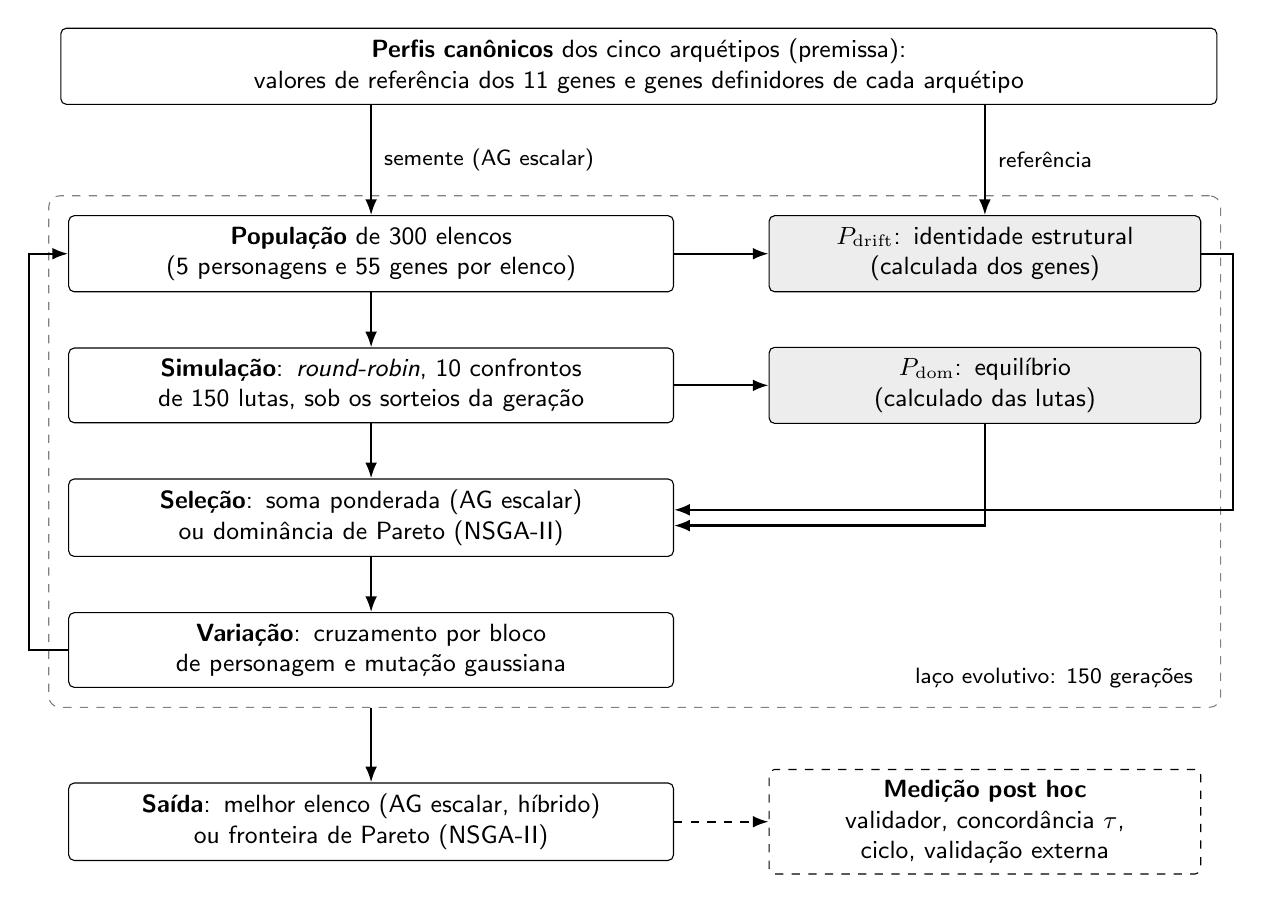
\begin{tikzpicture}[
        font=\small,
        caixa/.style={draw, rounded corners=2pt, align=center, inner sep=4pt, text width=#1},
        caixa/.default=7.4cm,
        objetivo/.style={draw, rounded corners=2pt, align=center, inner sep=4pt, text width=5.2cm, fill=black!7},
        seta/.style={-{Latex[length=2mm]}, thick},
        tracejada/.style={-{Latex[length=2mm]}, dashed, thick},
        faixa/.style={draw=black!50, dashed, rounded corners=4pt, inner sep=7pt},
        rotulo/.style={font=\footnotesize, fill=white, inner sep=1.5pt}
    ]
        \node[caixa=14.4cm] (canon) {\textbf{Perfis canônicos} dos cinco arquétipos (premissa):\\valores de referência dos 11 genes e genes definidores de cada arquétipo};

        \node[caixa, below=14mm of canon.south west, anchor=north west, xshift=1mm] (pop) {\textbf{População} de 300 elencos\\(5 personagens e 55 genes por elenco)};
        \node[caixa, below=7mm of pop] (sim) {\textbf{Simulação}: \textit{round-robin}, 10 confrontos\\de 150 lutas, sob os sorteios da geração};
        \node[caixa, below=7mm of sim] (sel) {\textbf{Seleção}: soma ponderada (AG escalar)\\ou dominância de Pareto (NSGA-II)};
        \node[caixa, below=7mm of sel] (var) {\textbf{Variação}: cruzamento por bloco\\de personagem e mutação gaussiana};

        \node[objetivo, right=12mm of pop] (drift) {$\Pdrift$: identidade estrutural\\(calculada dos genes)};
        \node[objetivo, right=12mm of sim] (dom) {$\Pdom$: equilíbrio\\(calculado das lutas)};

        \node[faixa, fit=(pop)(sim)(sel)(var)(drift)(dom)] (laco) {};
        \node[rotulo, anchor=south east] at ($(laco.south east)+(-3mm,2mm)$) {laço evolutivo: 150 gerações};

        \node[caixa, below=12mm of var] (saida) {\textbf{Saída}: melhor elenco (AG escalar, híbrido)\\ou fronteira de Pareto (NSGA-II)};
        \node[caixa=5.2cm, right=12mm of saida, dashed] (posthoc) {\textbf{Medição \textit{post hoc}}\\validador, concordância $\tau$,\\ciclo, validação externa};

        \draw[seta] (canon.south -| pop.north) -- node[rotulo, right=1mm] {semente (AG escalar)} (pop.north);
        \draw[seta] (canon.south -| drift.north) -- node[rotulo, right=1mm] {referência} (drift.north);
        \draw[seta] (pop) -- (sim);
        \draw[seta] (pop) -- (drift);
        \draw[seta] (sim) -- (dom);
        \draw[seta] (sim) -- (sel);
        \draw[seta] (drift.east) -- ++(4mm,0) |- ($(sel.east)+(0,1mm)$);
        \draw[seta] (dom.south) |- ($(sel.east)+(0,-1mm)$);
        \draw[seta] (sel) -- (var);
        \draw[seta] (var.west) -- ++(-5mm,0) |- (pop.west);
        \draw[seta] (laco.south -| saida.north) -- (saida.north);
        \draw[tracejada] (saida) -- (posthoc);
    \end{tikzpicture}
    \source
\end{figure}

Três algoritmos de busca operam sobre essa arquitetura: um algoritmo genético escalar, que combina os dois objetivos numa soma ponderada (\autoref{sec: ag_escalar}); o NSGA-II, que os trata como objetivos separados e devolve uma fronteira de Pareto (\autoref{sec: nsga2_metodo}); e um híbrido que encadeia os dois dentro do mesmo orçamento (\autoref{sec: hibrido}). Os três compartilham a representação, o combate, a função de avaliação e os operadores de variação. Os dois primeiros diferem na inicialização, na seleção e na formação de cada nova geração; o terceiro difere pelo encadeamento dos dois.

\section{Representação dos arquétipos}
\label{sec: representacao}

\subsection{Genes e limites}
\label{sub: genes}

Cada personagem é descrito por onze genes contínuos: oito atributos, que definem o que o personagem \textit{pode} fazer, e três pesos comportamentais, que definem o que ele \textit{tende} a fazer. A \autoref{tab: genes} lista os genes, o símbolo usado neste texto, o nome no código e o intervalo admitido na busca.

\begin{table}[htb]
    \caption{Genes de um personagem e limites do espaço de busca.}
    \label{tab: genes}
    \centering
    \small
    \begin{tabularx}{\textwidth}{l l l X}
        \toprule
        \textbf{Símbolo} & \textbf{Código} & \textbf{Limites} & \textbf{Significado} \\
        \midrule
        $\ghp$   & \texttt{hp}               & $[250;\, 450]$ & Pontos de vida iniciais. \\
        $\gdmg$  & \texttt{damage}           & $[15;\, 30]$   & Dano por golpe, fixo, em pontos de vida. \\
        $\gcool$ & \texttt{attack\_cooldown} & $[1;\, 5]$     & Intervalo entre golpes, em \textit{ticks}. \\
        $\grng$  & \texttt{range}            & $[5;\, 20]$    & Alcance do golpe, em unidades de campo. \\
        $\gspd$  & \texttt{speed}            & $[1;\, 5]$     & Deslocamento por \textit{tick}, em unidades de campo. \\
        $\gstun$ & \texttt{stun}             & $[0; 0{,}6]$ & Atordoamento causado por golpe, como fração do próprio $\gcool$. \\
        $\gkb$   & \texttt{knockback}        & $[0;\, 3]$     & Repulsão aplicada ao alvo por golpe, em unidades de campo. \\
        $\ggrab$ & \texttt{grab\_power}      & $[0;\, 1]$     & Poder de agarrão: quanto o golpe atravessa a guarda do alvo. \\
        \midrule
        $\wF$    & \texttt{w\_aggressiveness} & $[0;\, 1]$    & Peso da intenção de avançar (FRENTE). \\
        $\wR$    & \texttt{w\_retreat}        & $[0;\, 1]$    & Peso da intenção de recuar (RECUAR). \\
        $\wG$    & \texttt{w\_defend}         & $[0;\, 1]$    & Peso da intenção de guardar (GUARDA). \\
        \bottomrule
    \end{tabularx}
    \source
\end{table}

Os limites foram escolhidos para excluir configurações degeneradas que versões anteriores do modelo permitiam. O alcance máximo (20) é menor que a distância inicial entre os lutadores (50), de modo que nenhum personagem ataca antes de se mover. O atordoamento é expresso como fração do intervalo entre golpes do próprio atacante e limitado a 0,6. Assim, o alvo sempre recupera a ação antes do golpe seguinte, e o travamento permanente do oponente fica fora do espaço de busca. O intervalo de pontos de vida foi estreitado para eliminar o ``tanque'' de resistência extrema que a busca explorava. O teto da repulsão (3) fica acima do valor canônico do \textit{Zoner} (2), mas abaixo do ponto em que empurrar o oponente para fora do alcance se torna uma estratégia trivial. Os demais limites comportam os valores canônicos com folga dos dois lados, exceto cinco genes canônicos que ficam, por projeto, exatamente sobre um limite (\autoref{sub: canonicos}).

Os três pesos comportamentais não são probabilidades. A intenção de cada personagem é sorteada com probabilidade proporcional a eles (\autoref{sub: postura}), de modo que apenas a \textbf{razão} entre os três afeta o combate. Multiplicar os três pesos por uma constante positiva produz exatamente o mesmo personagem. Essa invariância de escala é levada em conta tanto na medida de identidade (\autoref{sub: drift}) quanto no validador de identidade (\autoref{chap: protocolo}).

\subsection{Perfis canônicos}
\label{sub: canonicos}

Os valores canônicos, na \autoref{tab: canonicos}, operacionalizam os cinco arquétipos descritos na \autoref{sec: arquetipos}. Cada arquétipo tem também um conjunto de \textbf{genes definidores}, destacados em negrito na tabela. São os genes em que o arquétipo ocupa, por projeto, um extremo do elenco, e que o tornam reconhecível: o \textit{Zoner} é o de maior alcance, maior repulsão e maior propensão a recuar; o \textit{Rushdown}, o mais rápido, o de menor intervalo entre golpes e o mais agressivo; o \textit{Combo Master}, o de maior atordoamento; o \textit{Grappler}, o de maior dano e maior poder de agarrão; o \textit{Turtle}, o de mais pontos de vida, maior intervalo entre golpes, menor velocidade e maior propensão a guardar.

\begin{table}[htb]
    \caption[Perfis canônicos dos cinco arquétipos]{Perfis canônicos dos cinco arquétipos. Em negrito, os genes definidores de cada um.}
    \label{tab: canonicos}
    \centering
    \footnotesize
    \setlength{\tabcolsep}{4pt}
    \begin{tabular}{l rrrrrrrr rrr}
        \toprule
        \textbf{Arquétipo} & $\ghp$ & $\gdmg$ & $\gcool$ & $\grng$ & $\gspd$ & $\gstun$ & $\gkb$ & $\ggrab$ & $\wF$ & $\wR$ & $\wG$ \\
        \midrule
        \textit{Zoner}        & 300 & 20 & 4 & \textbf{18} & 2,5 & 0,10 & \textbf{2,0} & 0,05 & 0,30 & \textbf{0,60} & 0,20 \\
        \textit{Rushdown}     & 320 & 16 & \textbf{1} & 10 & \textbf{5,0} & 0,10 & 1,0 & 0,20 & \textbf{0,90} & 0,05 & 0,10 \\
        \textit{Combo Master} & 350 & 18 & 3 & 10 & 3,0 & \textbf{0,55} & 0,5 & 0,30 & 0,70 & 0,05 & 0,20 \\
        \textit{Grappler}     & 400 & \textbf{27} & 4 & 8 & 2,0 & 0,30 & 0,5 & \textbf{0,90} & 0,70 & 0,10 & 0,40 \\
        \textit{Turtle}       & \textbf{450} & 15 & \textbf{5} & 13 & \textbf{1,5} & 0,20 & 1,0 & 0,15 & 0,20 & 0,40 & \textbf{0,70} \\
        \bottomrule
    \end{tabular}
    \source
\end{table}

Os perfis canônicos são a \textbf{premissa} do trabalho, não uma variável a otimizar, e foram declarados finais antes da bateria experimental. O critério que os aceitou foi escrito e medido: devem ser coerentes com a descrição funcional de cada arquétipo (satisfazem as 23 asserções do validador de identidade, descrito no \autoref{chap: protocolo}), devem ser distintos entre si e devem ser \textbf{desequilibrados de propósito}, para que exista algo a equilibrar. O terceiro critério é cumprido com folga: no elenco canônico o \textit{Rushdown} vence praticamente todas as suas lutas e o \textit{Turtle} praticamente nenhuma (\autoref{chap: resultados}). Cinco genes canônicos ficam exatamente sobre um limite do espaço de busca: os pontos de vida, o dano e o intervalo entre golpes do \textit{Turtle}, e a velocidade e o intervalo entre golpes do \textit{Rushdown}. A busca só pode afastá-los desse extremo para dentro do intervalo, o que é coerente com o papel de extremo que esses genes cumprem na identidade dos dois arquétipos.

Traduzidos em probabilidades de intenção, os pesos canônicos expressam os estilos esperados. O \textit{Rushdown} avança em 86\% das intenções sorteadas; o \textit{Zoner} recua em 55\%; o \textit{Turtle} guarda em 54\%.

\subsection{O indivíduo}
\label{sub: individuo}

A unidade manipulada pela busca é o \textbf{elenco completo}, não o personagem isolado. A taxa de vitória de qualquer personagem depende simultaneamente dos outros quatro, e a aptidão de um personagem sozinho não tem definição operacional. Cada indivíduo é, portanto, um vetor
\begin{equation}
    \label{eq: individuo}
    \mathbf{x} = \left(\mathbf{g}_{\mathrm{Z}}, \mathbf{g}_{\mathrm{R}}, \mathbf{g}_{\mathrm{C}}, \mathbf{g}_{\mathrm{G}}, \mathbf{g}_{\mathrm{T}}\right) \in \mathbb{R}^{55},
\end{equation}
em que $\mathbf{g}_a \in \mathbb{R}^{11}$ reúne os genes do personagem que ocupa o papel do arquétipo $a$. O papel é fixo: o primeiro bloco é sempre o \textit{Zoner} do elenco, e o desvio desse bloco é sempre medido contra o perfil canônico do \textit{Zoner}. O vetor canônico completo, formado pelos cinco perfis da \autoref{tab: canonicos}, é denotado por $\mathbf{c}$.

\section{Modelo de combate}
\label{sec: combate}

O combate é uma abstração deliberada dos jogos de luta. Não representa quadros de animação, sequências de entrada nem ataques de tipos diferentes. Representa o que é necessário para que os onze genes tenham efeito mensurável e para que os estilos dos arquétipos (pressão, controle de espaço, atrito, agarrão, travamento) possam existir como estratégias. As decisões de modelagem descritas nesta seção foram auditadas com um critério explícito: cada gene deve mover o desfecho das lutas de forma monótona e visível para a busca. As medições que motivaram cada decisão são citadas junto dela. O critério orientou o projeto do combate, mas não vale em qualquer ponto do espaço de busca: num elenco já equilibrado e com o passo de mutação adotado, dois dos três pesos comportamentais ficam abaixo do piso de ruído (\autoref{sub: res_sensibilidade}).

\subsection{Campo e escala de tempo}
\label{sub: campo}

A luta ocorre num campo unidimensional de comprimento $L = 100$ unidades, com os lutadores começando a uma distância $d_0 = 50$, nas posições 25 e 75. Um lutador nunca ultrapassa o outro: o da esquerda permanece à esquerda durante toda a luta.

O tempo é discreto. A unidade de projeto é o \textit{tick}, e cada \textit{tick} é subdividido em $S = 5$ sub-\textit{ticks}, que são a unidade real da simulação. O deslocamento por sub-\textit{tick} é $\gspd/S$, e os intervalos de tempo derivados dos genes são convertidos em sub-\textit{ticks} pela regra da \autoref{sub: resto}. A subdivisão existe para que os genes temporais tenham resolução fina: com \textit{ticks} inteiros, $\gcool \in [1;\, 5]$ teria apenas cinco efeitos distintos. A luta tem duração máxima de 2500 sub-\textit{ticks} (500 \textit{ticks}). O limite funciona apenas como trava de segurança: nas medições feitas para este texto, \koTaxa{} das lutas terminaram por nocaute, com duração média de cerca de \duracaoMediaSubticks{} sub-\textit{ticks}, tanto no elenco canônico quanto em elencos evoluídos e em elencos sorteados ao acaso.

\subsection{Dois canais de ação}
\label{sub: canais}

A decisão central do modelo é separar o movimento do ataque em dois canais independentes. A \textbf{postura} do lutador (avançar, recuar ou defender) é escolhida por uma política estocástica. O \textbf{ataque} não é escolhido: é uma regra de resolução, que dispara sempre que três condições valem ao mesmo tempo, a saber, o intervalo desde o golpe anterior terminou, o oponente está ao alcance e a postura não é de defesa. Avançar e recuar permitem golpear; apenas defender abre mão do golpe.

A separação é o que torna o controle de espaço uma estratégia. Em jogos de luta, ``zonear'' é atacar enquanto se mantém a distância, e um modelo em que atacar e recuar são ações mutuamente exclusivas não consegue representar isso. Numa versão anterior do modelo, com uma única ação por sub-\textit{tick}, recuar significava abrir mão do dano. A auditoria do combate mediu a consequência num par de teste (um personagem de alcance 20 contra um de alcance 6 e velocidade máxima): o personagem de longo alcance perdia 100\% das lutas \textit{independentemente} do seu alcance e da sua repulsão, os dois genes que definem o \textit{Zoner}. A repulsão chegava a ter efeito negativo, pois empurrar o alvo para fora do próprio alcance obrigava o atacante a persegui-lo. Com os dois canais, o mesmo personagem passou a vencer 49\% das lutas, e varrer a repulsão ao longo do seu intervalo passou a mover a taxa de vitória de 27\% para 72\%, de forma monótona.

\subsection{Decisão da postura}
\label{sub: postura}

A cada sub-\textit{tick}, cada lutador determina sua postura em duas etapas, resumidas no \autoref{quad: intencao}. Primeiro, se não houver uma intenção vigente, sorteia uma entre FRENTE, RECUAR e GUARDA, com probabilidades proporcionais aos seus pesos:
\begin{equation}
    \label{eq: intencao}
    \Pr(\text{FRENTE}) = \frac{\wF}{\wF + \wR + \wG}, \quad
    \Pr(\text{RECUAR}) = \frac{\wR}{\wF + \wR + \wG}, \quad
    \Pr(\text{GUARDA}) = \frac{\wG}{\wF + \wR + \wG}.
\end{equation}
Se os três pesos forem nulos, a intenção é GUARDA. A intenção sorteada é mantida por $n_{\mathrm{p}} = 5$ sub-\textit{ticks} antes de um novo sorteio. Depois, a intenção é traduzida em postura.

\begin{quadro}[htb]
    \caption{Tradução da intenção sorteada na postura do sub-\textit{tick}.}
    \label{quad: intencao}
    \centering
    \small
    \begin{tabularx}{\textwidth}{l l l X}
        \toprule
        \textbf{Intenção} & \textbf{Condição} & \textbf{Postura} & \textbf{Pode golpear?} \\
        \midrule
        FRENTE & sempre & avanço & sim \\
        RECUAR & há espaço atrás & recuo & sim \\
        RECUAR & encurralado na borda & defesa (forçada) & não \\
        GUARDA & sempre & defesa & não \\
        \midrule
        qualquer & ninguém alcança ninguém (impasse) & avanço (imposto) & sim \\
        qualquer & atordoado & nenhuma (perde o sub-\textit{tick}) & não \\
        \bottomrule
    \end{tabularx}
    \source
\end{quadro}

A política é deliberadamente estocástica e proporcional. Uma política determinística, que escolhesse sempre a ação de maior peso, faria dos pesos variáveis categóricas: só a ordem entre eles importaria, e toda mutação que não invertesse essa ordem seria invisível para a busca. Sob o sorteio proporcional da \autoref{eq: intencao}, qualquer variação num peso produz variação proporcional na frequência da intenção correspondente, e a busca tem sinal contínuo sobre os três genes.

A persistência da intenção modela o compromisso de uma decisão tática. Sem ela, o lutador sortearia uma intenção nova a cada sub-\textit{tick} e oscilaria entre avançar e recuar sem relação com qualquer comportamento estratégico. O valor $n_{\mathrm{p}} = 5$ é exatamente um \textit{tick} e exatamente o intervalo entre golpes do atacante mais rápido possível ($\gcool = 1$). Assim, quem sorteia GUARDA abre mão de exatamente uma janela de ataque. O valor foi também medido: comparado a $n_{\mathrm{p}} = 10$, ele melhorou a razão entre sinal e ruído da análise de sensibilidade em todos os oito atributos, com ganhos de 25\% a 81\%, porque mais decisões independentes por luta aumentam o efeito de cada gene e reduzem a variância do desfecho ao mesmo tempo. Durante um atordoamento a intenção fica suspensa: o lutador não age, e o contador de persistência não avança.

A intenção sorteada vale sempre, com uma única exceção, o \textbf{impasse}. Quando a distância supera o alcance dos dois lutadores, ninguém ameaça ninguém, e o avanço é imposto (e o contador de persistência é zerado). Sem essa regra, dois personagens de estilo passivo recuariam cada um para a sua borda e a luta acabaria por tempo sem um único golpe: a auditoria mediu 100\% de lutas encerradas por tempo no confronto entre \textit{Zoner} e \textit{Turtle} canônicos. A regra não afeta o controle de espaço, porque só vale quando nenhum dos dois alcança o outro. Um lutador que está ao alcance do oponente continua livre para recuar.

Recuar contra a borda do campo não é possível. Quando a intenção é RECUAR e não há espaço, a postura resultante é de defesa. O modelo registra essa defesa como \textbf{forçada}, distinta da defesa escolhida por GUARDA, para que a geometria do campo não contamine as métricas de comportamento defensivo usadas na medição de identidade (\autoref{chap: protocolo}).

\subsection{Movimento e colisão}
\label{sub: movimento}

Os dois lutadores se movem simultaneamente, ambos a partir das posições do início do sub-\textit{tick}. O avanço aproxima o lutador do oponente e o recuo o afasta, sempre com passo $\gspd/S$ e sempre limitado ao campo. Se os dois deslocamentos fizessem os corpos se cruzarem, ambos param no ponto em que se encontrariam. Sem a colisão, os corpos se atravessavam em média 134 vezes por luta no elenco canônico, a distância oscilava em torno de zero e o alcance perdia efeito no corpo a corpo.

\subsection{Resolução do ataque}
\label{sub: ataque}

Após o movimento, cada lutador golpeia se estiver em postura de avanço ou recuo, se seu temporizador de recarga estiver zerado e se a distância \textit{após o movimento} não exceder seu alcance. Os dois ataques são resolvidos com a mesma distância, de modo que nenhum lado golpeia ``primeiro''. Um ataque cujas condições não se cumprem simplesmente não ocorre e não consome recarga. Um golpe do lutador $i$ sobre o lutador $j$ tem quatro efeitos.

\textbf{Dano.} O dano é fixo, sem variância por golpe. O único modificador é a postura do alvo:
\begin{equation}
    \label{eq: dano}
    \mathrm{dano}_{i \to j} = \gdmg_i \cdot \mu_{ij},
    \qquad
    \mu_{ij} =
    \begin{cases}
        \rho + \ggrab_i, & \text{se } j \text{ está em defesa},\\
        1, & \text{caso contrário},
    \end{cases}
\end{equation}
em que $\rho = 0{,}6$ é o multiplicador da guarda (a defesa reduz o dano em 40\%). O gene de agarrão soma-se a esse multiplicador. Com $\ggrab_i = 0$, a guarda do alvo oferece a redução completa; no ponto neutro $\ggrab_i = 1 - \rho = 0{,}4$, a guarda é exatamente anulada; acima dele, defender passa a ser \textit{pior} do que não defender, até o teto de $1{,}6\times$ o dano. Entre os perfis canônicos, apenas o \textit{Grappler} ($\ggrab = 0{,}9$, multiplicador $1{,}5$) está acima do ponto neutro.

O agarrão foi modelado dessa forma por duas razões. Primeiro, em jogos de luta ele é o recurso clássico contra quem bloqueia, e a \autoref{eq: dano} só lhe dá efeito contra um alvo em defesa: contra quem avança ou recua, $\ggrab$ não altera nada. Segundo, ele não é uma quarta ação escolhida, mas uma condicional na resolução do golpe. O espaço de políticas continua o mesmo, sem um quarto peso comportamental.

A ausência de variância no dano também é deliberada. Ruído aditivo no dano reduziria o efeito de pequenas mutações abaixo do ruído binomial que a política estocástica já produz, sem acrescentar realismo relevante ao nível de abstração do modelo. A estocasticidade fica restrita ao único lugar em que modela incerteza estratégica: o sorteio da intenção.

\textbf{Atordoamento.} O alvo perde os próximos $n^{\mathrm{stun}}_i$ sub-\textit{ticks}, em média
\begin{equation}
    \label{eq: stun}
    \mathbb{E}\left[n^{\mathrm{stun}}_i\right] = \gstun_i \cdot \gcool_i \cdot S.
\end{equation}
Um atordoamento novo só substitui o vigente se for mais longo; os dois não se somam. Como $\gstun_i \le 0{,}6$, o atordoamento dura sempre menos que o intervalo entre golpes do próprio atacante, e o alvo recupera a ação antes do golpe seguinte.

\textbf{Repulsão.} O alvo é empurrado $\gkb_i$ unidades para longe do atacante, limitado à borda do campo.

\textbf{Recarga.} O atacante só volta a golpear depois de $n^{\mathrm{cd}}_i$ sub-\textit{ticks}, em média
\begin{equation}
    \label{eq: periodo}
    \mathbb{E}\left[n^{\mathrm{cd}}_i\right] = \gcool_i \cdot S.
\end{equation}

\subsection{Temporizadores com resto acumulado}
\label{sub: resto}

A \autoref{eq: stun} e a \autoref{eq: periodo} dão quantidades contínuas, mas os temporizadores contam sub-\textit{ticks} inteiros. Arredondar cada golpe isoladamente deixaria os dois genes em degraus. Com $\gcool = 1$, por exemplo, o atordoamento teria apenas quatro efeitos distintos em todo o intervalo $[0; 0{,}6]$, e mutações dentro de um degrau seriam invisíveis para a busca. O modelo converte cada quantidade contínua $q$ em inteiro por \textbf{difusão de erro}, carregando o resto de um golpe para o seguinte:
\begin{equation}
    \label{eq: resto}
    n_k = \left\lfloor q + e_{k-1} \right\rfloor,
    \qquad
    e_k = q + e_{k-1} - n_k,
    \qquad
    e_0 = 0{,}5.
\end{equation}
Um intervalo de 6,5 sub-\textit{ticks}, por exemplo, produz a sequência 7, 6, 7, 6, $\ldots$, com média exata 6,5. Cada lutador mantém um resto para a recarga e outro para o atordoamento. O efeito dos genes torna-se contínuo em média, e o combate continua determinístico dado o sorteio de intenções, sem uma segunda fonte de acaso. A mudança foi medida no gene de atordoamento de um \textit{Rushdown} evoluído: varrido em 31 valores, ele produzia apenas 5 taxas de vitória distintas antes da difusão de erro e 27 depois.

Os temporizadores são decrementados ao fim de cada sub-\textit{tick}, exceto os que foram renovados por um golpe naquele mesmo sub-\textit{tick}. O sub-\textit{tick} do próprio golpe conta como o primeiro do intervalo, de modo que a recarga é iniciada em $n^{\mathrm{cd}}_i - 1$ e o golpe seguinte ocorre exatamente $n^{\mathrm{cd}}_i$ sub-\textit{ticks} depois.

\subsection{Desfecho da luta}
\label{sub: desfecho}

A luta termina quando os pontos de vida de um lutador chegam a zero (nocaute) ou quando se esgota a duração máxima. Neste último caso vence quem conserva a maior \textit{fração} dos pontos de vida iniciais. Se os dois terminam com a mesma fração, o que inclui o nocaute duplo no mesmo sub-\textit{tick}, a luta é um \textbf{empate}, contado como meia vitória para cada lado.

O empate não é detalhe. Sem ele, o desempate precisaria favorecer um dos lados, e o lado favorecido seria sempre o mesmo, pois a avaliação (\autoref{sec: avaliacao}) põe o arquétipo de menor índice sempre à esquerda. Numa versão anterior, que dava o desempate ao lado esquerdo, o espelho do \textit{Rushdown} canônico, que por simetria deveria dar 50\%, dava 54,9\% ao lado esquerdo: um viés sistemático na grandeza que a aptidão otimiza.

\subsection{Síntese de um sub-\textit{tick}}
\label{sub: subtick}

O \autoref{alg: subtick} reúne as regras desta seção. O único passo estocástico é o sorteio da intenção. Todo o resto é determinístico dado esse sorteio, o que permite reproduzir uma luta exatamente a partir da semente do gerador de números aleatórios (\autoref{sec: ruido}).

\begin{algoritmo}[htb]
    \caption{Um sub-\textit{tick} do combate.}
    \label{alg: subtick}
    \begin{algorithmic}[1]
        \Require para cada lutador $L$: posição $x_L$, pontos de vida $h_L$, temporizadores de recarga $c_L$ e de atordoamento $a_L$, intenção vigente $I_L$ e persistência restante $k_L$
        \Function{Postura}{$L$, $O$, $d$}
            \If{$a_L > 0$}
                \State \Return nenhuma \Comment{atordoado: perde o sub-\textit{tick}}
            \ElsIf{$d > \grng_L$ \textbf{e} $d > \grng_O$}
                \State $k_L \gets 0$
                \State \Return avanço \Comment{impasse}
            \EndIf
            \If{$k_L = 0$}
                \State sorteia $I_L$ segundo a \autoref{eq: intencao}; \quad $k_L \gets n_{\mathrm{p}}$
            \EndIf
            \State $k_L \gets k_L - 1$
            \If{$I_L = $ FRENTE}
                \State \Return avanço
            \ElsIf{$I_L = $ RECUAR}
                \State \Return recuo, se houver espaço atrás; senão, defesa forçada
            \EndIf
            \State \Return defesa
        \EndFunction
        \Statex
        \State $d \gets |x_B - x_A|$
        \State $\sigma_A \gets \Call{Postura}{A, B, d}$; \quad $\sigma_B \gets \Call{Postura}{B, A, d}$
        \State move $A$ e $B$ simultaneamente segundo $\sigma_A$ e $\sigma_B$, sem atravessamento
        \State $d \gets |x_B - x_A|$ \Comment{distância após o movimento}
        \For{cada par $(L, O) \in \{(A, B), (B, A)\}$} \Comment{resolução simultânea}
            \If{$\sigma_L \in \{\text{avanço}, \text{recuo}\}$ \textbf{e} $c_L = 0$ \textbf{e} $d \le \grng_L$}
                \State $h_O \gets \max\left(0,\, h_O - \gdmg_L \cdot \mu_{LO}\right)$ \Comment{\autoref{eq: dano}}
                \State $a_O \gets \max\left(a_O,\, n^{\mathrm{stun}}_L\right)$ \Comment{\autoref{eq: stun} e \autoref{eq: resto}}
                \State empurra $O$ em $\gkb_L$ para longe de $L$, limitado ao campo
                \State $c_L \gets n^{\mathrm{cd}}_L - 1$ \Comment{\autoref{eq: periodo} e \autoref{eq: resto}}
            \EndIf
        \EndFor
        \State decrementa os temporizadores positivos que não foram renovados neste sub-\textit{tick}
    \end{algorithmic}
    \source
\end{algoritmo}

\section{Avaliação de um elenco}
\label{sec: avaliacao}

Um elenco é avaliado por \textbf{\textit{round-robin} completo}: cada um dos $\binom{5}{2} = 10$ pares de personagens distintos luta $N = 150$ vezes. O par $(i, j)$, com $i < j$, é simulado sempre com $i$ à esquerda. A avaliação completa custa, portanto, 1500 lutas.

Das lutas derivam três grandezas. A \textbf{taxa de vitória do par}, $p_{ij}$, é a fração de lutas vencidas por $i$ contra $j$, com cada empate contado como meia vitória; por construção, $p_{ji} = 1 - p_{ij}$. A \textbf{taxa de vitória global} de um personagem é a média das suas taxas de vitória nos quatro confrontos:
\begin{equation}
    \label{eq: wr_global}
    \bar{p}_i = \frac{1}{4} \sum_{j \neq i} p_{ij}.
\end{equation}
A terceira grandeza é a \textbf{decisividade} de um par, que mede a margem das lutas, e não quem as vence. Cada luta recebe um escore contínuo $s \in [0;\, 1]$, do ponto de vista de $i$:
\begin{equation}
    \label{eq: escore}
    s =
    \begin{cases}
        \tfrac{1}{2} + \tfrac{1}{2}\, f_i, & \text{se } i \text{ vence por nocaute},\\[2pt]
        \tfrac{1}{2} - \tfrac{1}{2}\, f_j, & \text{se } j \text{ vence por nocaute},\\[2pt]
        f_i / (f_i + f_j), & \text{se a luta acaba por tempo},\\[2pt]
        \tfrac{1}{2}, & \text{se há empate},
    \end{cases}
\end{equation}
em que $f_i$ é a fração dos pontos de vida iniciais que $i$ conserva ao fim da luta. Um nocaute em que o vencedor sai intacto dá escore próximo de 1; um nocaute conquistado no limite dá escore próximo de 0,5. A decisividade do par é a margem média:
\begin{equation}
    \label{eq: decisividade}
    D_{ij} = \frac{1}{N} \sum_{k=1}^{N} \left| s_k - \tfrac{1}{2} \right|.
\end{equation}
Como, nas medições, toda luta terminou por nocaute (\autoref{sub: campo}), $D_{ij}$ é, na prática, metade da fração média de pontos de vida com que o vencedor termina. Valor alto significa que as lutas do par são massacres, qualquer que seja o lado que os vença.

O número de lutas por par equilibra custo e precisão. A 150 lutas, o desvio-padrão binomial de uma taxa de vitória próxima de 50\% é cerca de 4 pontos percentuais, uma fração pequena da tolerância de 15 pontos que define um confronto desequilibrado (\autoref{sub: dominancia}). A fonte de imprecisão que mais afetava os resultados não era o tamanho da amostra de cada avaliação, mas o reaproveitamento da mesma amostra ao longo da busca, tratado na \autoref{sec: ruido}.

\section{Função de aptidão}
\label{sec: aptidao}

\subsection{O que a aptidão pode codificar}
\label{sub: premissa}

A pergunta de pesquisa contém um risco de circularidade. Se a função de aptidão recompensasse diretamente a estrutura que se quer observar, observá-la ao fim da busca não provaria nada: o algoritmo a exibiria porque foi pago para exibi-la. A formulação adotada evita esse risco separando dois tipos de informação:

\begin{itemize}
    \item a \textbf{premissa} é o que cada arquétipo \textit{é}: os perfis canônicos e os genes definidores. Ela é dada pela convenção do gênero, é anterior à pergunta de equilíbrio e independente dela. A premissa \textbf{pode} entrar na aptidão;
    \item a \textbf{resposta} é o que a pergunta quer descobrir: quem vence quem, e se equilíbrio e identidade são compatíveis. A resposta \textbf{nunca} entra na aptidão; é medida \textit{post hoc}.
\end{itemize}

``O \textit{Zoner} é o personagem definido pelo alcance'' é premissa. ``O \textit{Zoner} deve vencer o \textit{Grappler}'' é resposta. Daí a assimetria da formulação: a identidade estrutural é um termo da aptidão, e o ciclo de vantagens do \autoref{quad: ciclo_canonico} não é.

A identidade entra como \textbf{penalidade}, não como restrição, e a distinção é empírica, não retórica. Uma restrição proibiria certos resultados, e não haveria nada a medir além do que foi imposto. Uma penalidade dá um custo à perda de identidade e deixa o algoritmo livre para pagá-lo quando o ganho de equilíbrio compensar. O \autoref{chap: resultados} mostra que ele de fato paga: com o termo de identidade ativo durante toda a busca, o elenco evoluído perde parte relevante da identidade medida pelo validador. O termo existe e pode perder.

Por fim, a identidade que responde à pergunta, isto é, a identidade \textit{funcional}, sobre como cada personagem joga, não é medida pelo termo da aptidão. É medida por réguas comportamentais aplicadas \textit{post hoc}, que a busca nunca vê (\autoref{chap: protocolo}). O \autoref{quad: otimizado} resume o que é otimizado e o que é apenas medido.

\begin{quadro}[htb]
    \caption{O que a busca otimiza e o que é medido apenas \textit{post hoc}.}
    \label{quad: otimizado}
    \centering
    \small
    \begin{tabularx}{\textwidth}{X l l}
        \toprule
        \textbf{Grandeza} & \textbf{Na aptidão?} & \textbf{Onde é tratada} \\
        \midrule
        Desvio ponderado em relação ao perfil canônico ($\Pdrift$) & sim & \autoref{sub: drift} \\
        Desequilíbrio global, \textit{hard counters} e decisividade ($\Pdom$) & sim & \autoref{sub: dominancia} \\
        Taxa de vitória de cada par exatamente em 50\% & não & -- \\
        Identidade funcional (validador comportamental, concordância $\tau$) & não & \autoref{chap: protocolo} \\
        Ciclo canônico de vantagens & não & \autoref{chap: protocolo} \\
        Robustez a regras de combate não vistas & não & \autoref{chap: protocolo} \\
        \bottomrule
    \end{tabularx}
    \source
\end{quadro}

\subsection{Identidade estrutural: o desvio ponderado}
\label{sub: drift}

A penalidade de desvio $\Pdrift$ mede quanto os genes de cada personagem se afastaram do perfil canônico do seu arquétipo. Para o gene $k$ do personagem do arquétipo $a$, o desvio normalizado é
\begin{equation}
    \label{eq: desvio_gene}
    e_{a,k} = \frac{\tilde{g}_{a,k} - c_{a,k}}{u_k - \ell_k},
\end{equation}
em que $[\ell_k;\, u_k]$ é o intervalo admitido para o gene (\autoref{tab: genes}) e $c_{a,k}$ é o valor canônico. O desvio do personagem é a raiz da média ponderada dos quadrados, e a penalidade do elenco é a média sobre os cinco personagens:
\begin{equation}
    \label{eq: drift}
    \delta_a = \sqrt{\frac{\sum_{k=1}^{11} \omega_{a,k}\, e_{a,k}^2}{\sum_{k=1}^{11} \omega_{a,k}}},
    \qquad
    \Pdrift(\mathbf{x}) = \frac{1}{5} \sum_{a} \delta_a,
    \qquad
    \omega_{a,k} =
    \begin{cases}
        3, & \text{se } k \text{ é gene definidor de } a,\\
        1, & \text{caso contrário.}
    \end{cases}
\end{equation}
$\Pdrift$ vale zero no elenco canônico e cresce com o afastamento; não depende de simulação e, portanto, é calculado sem ruído. Três escolhas da \autoref{eq: drift} merecem justificativa.

\textbf{Normalização pela amplitude do intervalo.} Dividir o desvio pela amplitude $u_k - \ell_k$, e não pelo limite superior $u_k$, evita subestimar genes cujo limite inferior é alto. Os pontos de vida variam de 250 a 450: afastar-se 162 pontos é mover-se 81\% do intervalo, mas apenas 36\% do máximo. A normalização pela amplitude foi a correção que fez a ordenação dos elencos por $\Pdrift$ concordar com a ordenação pelo validador de identidade.

\textbf{Peso dos genes definidores.} Na soma dos quadrados, um desvio no alcance do \textit{Zoner} pesa três vezes o mesmo desvio no seu atordoamento. A ponderação traduz a premissa de que alguns genes definem o arquétipo mais que outros, sem transformá-la em restrição. Na medição que a motivou, ela ampliou a separação entre elencos de identidade distinta de 0,017 para 0,043 unidades de $\Pdrift$. Pesos maiores ampliariam pouco essa separação e tornariam quase gratuitos os genes não definidores.

\textbf{Pesos comportamentais reescalados.} Como só a razão entre os três pesos afeta o combate (\autoref{sub: genes}), comparar os valores crus cobraria desvio por uma diferença sem efeito. Antes da comparação, os três pesos do personagem são multiplicados por um fator comum que iguala sua soma à soma canônica:
\begin{equation}
    \label{eq: reescala}
    \tilde{w}_{a,m} = w_{a,m} \cdot \frac{\sum_{m'} c_{a,m'}}{\sum_{m'} w_{a,m'}}, \qquad m, m' \in \{\mathrm{F}, \mathrm{R}, \mathrm{G}\}.
\end{equation}
Os atributos entram sem alteração ($\tilde{g}_{a,k} = g_{a,k}$). Sem a reescala, 7,5\% do desvio médio de um elenco evoluído correspondia a essa diferença invisível: a busca inflava a escala dos pesos e a penalidade cobrava pela inflação.

A agregação por raiz da média dos quadrados, aqui e nos termos de equilíbrio, faz os afastamentos grandes pesarem mais que os pequenos, de modo que a busca não consegue esconder um gene muito deslocado atrás de uma média confortável. $\Pdrift$ é também o mecanismo que impede a solução trivial do equilíbrio. Cinco cópias do mesmo personagem são perfeitamente simétricas, mas quatro delas estão longe do próprio perfil canônico, e a penalidade as cobra.

\subsection{Equilíbrio: a penalidade de dominância}
\label{sub: dominancia}

A penalidade de dominância $\Pdom$ traduz em número a noção de equilíbrio adotada. Ela parte de uma escolha conceitual. Equilíbrio \textbf{não} é toda taxa de vitória de par igual a 50\%. Esse equilíbrio ``plano'' é incompatível, por construção, com uma estrutura de vantagens recíprocas, em que alguns personagens vencem outros; otimizá-lo destruiria qualquer ciclo e faria dessa destruição um artefato do objetivo, não um achado. Equilíbrio, aqui, é \textbf{nenhum arquétipo dominar o elenco}. Um personagem com taxa global de 50\% pode vencer dois confrontos e perder dois, e é nesse espaço que um ciclo de vantagens pode existir. $\Pdom$ combina um termo primário e dois secundários:
\begin{equation}
    \label{eq: dominancia}
    \Pdom(\mathbf{x}) = \beta_{\mathrm{g}}\, \tglob + \beta_{\mathrm{c}}\, \tcap + \beta_{\mathrm{d}}\, \tdec,
    \qquad
    (\beta_{\mathrm{g}}, \beta_{\mathrm{c}}, \beta_{\mathrm{d}}) = (1;\, 0{,}5;\, 0{,}5).
\end{equation}
Cada termo varia entre 0 e 1, de modo que $\Pdom \in [0;\, 2]$.

\textbf{Termo primário: desequilíbrio global.} Mede o afastamento de cada personagem da taxa global de 50\%, agregado por raiz da média dos quadrados sobre os cinco:
\begin{equation}
    \label{eq: termo_global}
    \tglob = \sqrt{\frac{1}{5} \sum_{i} \left( \frac{|\bar{p}_i - 1/2|}{1/2} \right)^2}.
\end{equation}

\textbf{Termo secundário: \textit{hard counters}.} O termo global sozinho admitiria confrontos esmagadores, desde que compensados em outros pares. Um confronto é chamado aqui de \textit{hard counter} quando $|p_{ij} - 1/2| > \kappa$, isto é, quando um lado vence mais de 65\% das lutas. O termo penaliza apenas o excesso acima dessa tolerância:
\begin{equation}
    \label{eq: termo_cap}
    \tcap = \sqrt{\frac{1}{10} \sum_{i<j} \left( \frac{\max\left(0,\, |p_{ij} - 1/2| - \kappa\right)}{1/2 - \kappa} \right)^2},
    \qquad \kappa = 0{,}15.
\end{equation}
Dentro da faixa $[0{,}35;\, 0{,}65]$ o par não é penalizado, e uma aresta de ciclo pode existir como vantagem.

A tolerância $\kappa$ foi ancorada na convenção do gênero. Tabelas de confrontos de jogos de luta são expressas como pares de inteiros que somam 10: 5-5, 6-4, 7-3, 8-2. Em $|p - 1/2|$, esses pontos valem 0; 0,10; 0,20 e 0,30. Na leitura corrente da comunidade, 6-4 é uma vantagem saudável e 7-3 já é um \textit{counter}. A tolerância precisa, portanto, admitir 0,10 e barrar 0,20. Ela também não pode coincidir com um ponto da grade: com o ruído binomial da medição, um limiar colado a um valor legítimo o reprovaria em metade das avaliações. A \autoref{tab: cap} mostra, para as três escolhas candidatas, a probabilidade de um confronto verdadeiramente 6-4 ser acusado e de um verdadeiramente 7-3 ser detectado, sob 150 lutas. Apenas $\kappa = 0{,}15$, o ponto médio entre 6-4 e 7-3, erra pouco nos dois sentidos.

\begin{table}[htb]
    \caption[Tolerância de \textit{hard counter} e erros de classificação]{Tolerância $\kappa$ de \textit{hard counter} e erros de classificação sob ruído binomial (150 lutas por par).}
    \label{tab: cap}
    \centering
    \small
    \begin{tabular}{c c c c}
        \toprule
        $\kappa$ & \textbf{Limiar} & \textbf{6-4 verdadeiro acusado} & \textbf{7-3 verdadeiro detectado} \\
        \midrule
        0,10 & 0,60 & 50,0\% & 99,6\% \\
        \textbf{0,15} & \textbf{0,65} & \textbf{10,6\%} & \textbf{90,9\%} \\
        0,20 & 0,70 & 0,6\% & 50,0\% \\
        \bottomrule
    \end{tabular}
    \source
\end{table}

\textbf{Termo secundário: decisividade.} Os termos anteriores olham para \textit{quem} vence. Nenhum deles detecta o caso em que os dois lados de um par se alternam em massacres: 55\% das lutas vencidas com folga por um lado e 45\% com folga pelo outro dão taxa de vitória próxima de 50\%, mas cada luta é decidida muito antes do fim. A decisividade da \autoref{eq: decisividade} detecta esse caso, porque mede a margem média $|s - 1/2|$, e não a margem da média. O termo penaliza a decisividade fora de uma faixa $[\varphi;\, \theta]$:
\begin{equation}
    \label{eq: termo_decis}
    \tdec = \sqrt{\frac{1}{10} \sum_{i<j} \left( \frac{\max(0,\, D_{ij} - \theta)}{1/2 - \theta} + \frac{\max(0,\, \varphi - D_{ij})}{\varphi} \right)^2},
    \qquad \theta = 0{,}20,\ \varphi = 0{,}02.
\end{equation}
O teto $\theta$ é o regularizador efetivo: $D_{ij} > 0{,}20$ significa que o vencedor termina, em média, com mais de 40\% dos pontos de vida. Numa medição sobre 18 elencos de referência, entre eles o canônico e elencos aleatórios, ele disparou em 57 dos 180 pares. O piso $\varphi$ é apenas uma guarda contra elencos degenerados, em que as lutas não chegam a ser decididas. Ele fica acima de um elenco degenerado construído para esse fim (dano mínimo, vida máxima, guarda permanente, $D \le 0{,}008$) e abaixo de qualquer par de personagens distintos. Um piso mais alto puniria lutas apertadas, que são justamente o que o termo primário busca, e empurraria a busca na direção oposta a ele.

A presença dos termos secundários foi decidida por medição. Numa varredura com os dois desligados, a busca atingiu o menor desequilíbrio global de todas as configurações testadas e, ainda assim, transformou em média 8,6 dos 10 pares em \textit{hard counters}. Remover apenas a decisividade elevou o número médio de \textit{hard counters} de 0,4 para 2,6. Os dois termos, portanto, sustentam a qualidade do equilíbrio mesmo quando valem zero no elenco final: um termo de guarda que termina em zero é um termo que cumpriu sua função. Já a repartição $0{,}5/0{,}5$ é uma escolha dentro de um compromisso medido. As alternativas que aumentavam o peso dos termos secundários eliminaram os \textit{hard counters} residuais, mas pagaram em identidade, com desvio maior e concordância comportamental com o canônico menor (\autoref{chap: protocolo}). A repartição adotada fica no ponto em que os termos secundários já sustentam o equilíbrio sem ainda dominar a identidade.

Os três termos compartilham duas propriedades. São \textbf{cegos à direção}: usam $|p - 1/2|$ e $|s - 1/2|$, e nada neles indica qual lado \textit{deveria} vencer um confronto. E são reportados separadamente em todos os arquivos de resultado que o sistema grava (os artefatos, \autoref{sec: reprodutibilidade}), porque perder no termo primário e perder num termo secundário de peso 0,5 são leituras opostas do mesmo valor de $\Pdom$.

\subsection{Formulações escalar e biobjetivo}
\label{sub: formulacoes}

Os dois termos definem as duas formulações usadas na busca. O algoritmo genético escalar maximiza
\begin{equation}
    \label{eq: aptidao_escalar}
    F(\mathbf{x}) = -\left( \lambda_{\mathrm{drift}}\, \Pdrift(\mathbf{x}) + \lambda_{\mathrm{dom}}\, \Pdom(\mathbf{x}) \right),
    \qquad \lambda_{\mathrm{drift}} = \lambda_{\mathrm{dom}} = 1,
\end{equation}
e o NSGA-II minimiza o vetor
\begin{equation}
    \label{eq: aptidao_vetorial}
    \mathbf{f}(\mathbf{x}) = \left( \Pdom(\mathbf{x}),\, \Pdrift(\mathbf{x}) \right)
\end{equation}
sem ponderação alguma. As duas formulações usam exatamente os mesmos dois termos, e a comparação entre os algoritmos não confunde método de busca com objetivo.

Na \autoref{eq: aptidao_escalar}, só a razão $\lambda_{\mathrm{drift}}/\lambda_{\mathrm{dom}}$ importa: a seleção por torneio é ordinal, e multiplicar os dois pesos por uma mesma constante não altera nenhuma decisão. O valor 1 foi escolhido por uma varredura dessa razão (\autoref{chap: protocolo}). Até $\lambda_{\mathrm{drift}} = 1$, o equilíbrio alcançado permanece praticamente constante enquanto a identidade melhora; acima de 1, o equilíbrio se degrada rapidamente. A razão unitária é o joelho dessa curva: entre os valores testados, é o maior peso de identidade que ainda não custa equilíbrio.

\section{Avaliação sob ruído}
\label{sec: ruido}

A aptidão de um elenco é uma variável aleatória, e a busca opera, portanto, sob avaliação ruidosa \cite{jin2005evolutionary}. $\Pdrift$ é exato, pois depende só dos genes, mas $\Pdom$ é estimado a partir de 1500 lutas estocásticas. Numa medição feita para este texto, em 30 sorteios independentes, o $\Pdom$ de um mesmo elenco evoluído varia com desvio-padrão de \ruidoDomDpTreino{} a 150 lutas por par, uma quantidade da mesma ordem do próprio valor de $\Pdom$ desses elencos. O modo como esse ruído é tratado define o que a busca realmente otimiza, e o protocolo adotado tem duas partes.

\textbf{Números aleatórios comuns dentro de uma geração.} Todos os indivíduos de uma mesma geração são avaliados sob a mesma sequência de sorteios, técnica de redução de variância conhecida como \textit{common random numbers} (CRN) \cite{law2015simulation}. Cada luta recebe uma semente própria, derivada da semente da geração, do índice do par e do índice da luta por uma função de espalhamento, a etapa final do gerador SplitMix64 \cite{steele2014fast}. Assim, a luta $k$ do par $m$ usa os mesmos sorteios em todos os indivíduos, independentemente de quantos sorteios as lutas anteriores consumiram. Os pares que não envolvem um personagem alterado saem idênticos entre dois indivíduos, e a diferença de aptidão entre eles deixa de conter o sorteio dessas lutas. O ruído não desaparece, porém. Quando um gene muda o que acontece numa luta, o resto dela se desenrola de outro modo, e os sorteios seguintes caem em estados diferentes. Medida sobre um elenco evoluído com um único gene deslocado de um desvio de mutação, a diferença de aptidão entre as duas versões ainda varia com desvio-padrão de \crnDpDiferenca{}. As consequências desse ruído residual para a seleção são discutidas na \autoref{sec: disc_ruido}.

\textbf{Rotação do \textit{stream} entre gerações.} A sequência de sorteios, ou \textit{stream}, muda a cada geração: a geração $g$ da execução de semente $r$ usa a semente-base $1000\,r + g$. Sem a rotação, as 150 gerações seriam avaliadas sobre uma única realização do gerador, e a população se ajustaria a ela, selecionando elencos que parecem equilibrados \textit{naqueles} sorteios. O efeito foi medido comparando o $\Pdom$ do melhor elenco dentro do laço com o mesmo elenco reavaliado em sorteios novos: a razão entre os dois caiu de 4,14 para 2,20 com a rotação, e melhorou nas cinco sementes testadas. A mesma regra que impede a confirmação de convergência de reutilizar os sorteios do treino (\autoref{sec: ag_escalar}) é, assim, aplicada à busca inteira.

A rotação tem dois custos declarados. O primeiro é computacional: os sobreviventes de uma geração, inclusive a elite, precisam ser reavaliados no \textit{stream} novo para que a comparação dentro da geração continue justa. O segundo é conceitual: a aptidão do melhor indivíduo oscila entre gerações, e a ``melhor aptidão já vista'' deixa de ser uma grandeza útil, pois seria o máximo de valores ruidosos e subiria por sorte. Por essa razão, o trabalho não usa critério de parada por estagnação.

\section{Algoritmo genético escalar}
\label{sec: ag_escalar}

O algoritmo genético escalar segue o esquema geracional clássico \cite{goldberg1989genetic, eiben2015introduction}, resumido no \autoref{alg: ag}.

\textbf{Inicialização.} A população de $M = 300$ elencos contém o elenco canônico e 299 elencos sorteados uniformemente dentro dos limites da \autoref{tab: genes}. Como o seu desvio é nulo, a aptidão do canônico ($F \approx -1{,}28$) fica entre as melhores da população inicial. Na geração inicial das 20 execuções da bateria, reproduzida para este texto, ele está sempre entre os \canonRankMax{} melhores dos 300 elencos, com posição mediana \canonRankMed{}, e é o melhor de todos em \canonMelhorN{} delas. Está, portanto, sempre dentro da elite. O seu desequilíbrio ($\Pdom \approx 1{,}28$), porém, é maior que o dos melhores elencos sorteados, e ele é superado assim que a população produz elencos mais equilibrados: na execução de semente 42, deixa a população na geração \canonSaiGer{}. Ele funciona como fonte de material genético próximo da premissa, sem garantia de sobreviver à seleção. A inicialização difere da do NSGA-II, e o efeito dessa diferença é medido por um braço de controle sem a semente canônica (\autoref{chap: protocolo}).

\textbf{Seleção.} Cada pai é o melhor de três indivíduos sorteados da população (torneio de tamanho 3).

\textbf{Cruzamento.} O cruzamento opera por \textbf{bloco de personagem}: cada um dos cinco personagens do filho é copiado integralmente de um dos dois pais, escolhido com probabilidade 1/2. Os atributos e os pesos de um mesmo personagem são sempre herdados juntos. Um cruzamento gene a gene poderia combinar a capacidade de um personagem com a estratégia de outro, produzindo configurações sem correspondência funcional. O custo dessa escolha é que a recombinação \textit{dentro} de um personagem fica a cargo apenas da mutação.

\textbf{Mutação.} Cada gene do filho sofre, com probabilidade 0,05, uma perturbação gaussiana de média zero, e o resultado é limitado ao intervalo do gene. O desvio-padrão da perturbação é 10\% da amplitude do intervalo nos atributos e 2,5\% nos pesos comportamentais. Em média, cerca de 2,75 dos 55 genes mudam por filho. A diferença entre os dois desvios expressa uma inércia deliberada: os atributos definem a capacidade do personagem, os pesos definem a sua estratégia, e mudanças bruscas de estratégia produziriam descontinuidades de comportamento incompatíveis com a noção de desvio gradual. O custo dessa inércia, medido depois, é discutido na \autoref{sec: disc_politica}.

\textbf{Elitismo.} Os 10\% melhores indivíduos da geração (30 elencos) passam sem alteração para a seguinte. A taxa é definida como fração da população, e não como contagem, para que execuções com população menor preservem a mesma pressão seletiva. O tamanho do torneio e a taxa de elitismo foram testados contra alternativas (\autoref{chap: protocolo}).

\textbf{Orçamento fixo e convergência como evento.} A execução percorre sempre as $G = 150$ gerações. A comparação com o NSGA-II exige isso: o NSGA-II não pode parar pelo mesmo critério, porque ``o elenco está equilibrado?'' não é pergunta que se faça a uma fronteira, e parar o escalar mais cedo tornaria impossível distinguir ``encontrou uma solução melhor'' de ``usou menos orçamento''. A convergência é, em vez disso, um \textbf{evento registrado}. Um elenco é considerado equilibrado quando
\begin{equation}
    \label{eq: equilibrado}
    \textsc{Equilibrado}(\mathbf{x}) \iff
    \max_{i} \left| \bar{p}_i - \tfrac{1}{2} \right| \le \varepsilon
    \ \wedge\
    \max_{i<j} \left| p_{ij} - \tfrac{1}{2} \right| \le \kappa,
    \qquad \varepsilon = 0{,}10,\ \kappa = 0{,}15,
\end{equation}
isto é, quando todo personagem tem taxa global entre 40\% e 60\% e nenhum par é \textit{hard counter}. O predicado não exige cada par em 50\%, pelas mesmas razões do termo primário de $\Pdom$. A geração de convergência $g^\star$ é a primeira em que o melhor elenco satisfaz a \autoref{eq: equilibrado} duas vezes: na avaliação do próprio laço e numa reavaliação com 200 lutas por par, sob um \textit{stream} que a busca nunca viu. Reavaliar sob os sorteios do treino não confirmaria nada, porque mediria a mesma realização do gerador com mais amostras. A confirmação independente recusa a maior parte dos disparos: na bateria experimental, das \gateDisparosAG{} vezes em que o melhor elenco pareceu equilibrado dentro do laço, \gateRecusasAG{} não sobreviveram à reavaliação.

\textbf{Saída.} Ao fim do orçamento, a execução devolve o melhor elenco da última população, avaliado sob o \textit{stream} da geração final, e a geração de convergência, se houver.

\begin{algoritmo}[htb]
    \caption{Algoritmo genético escalar.}
    \label{alg: ag}
    \begin{algorithmic}[1]
        \Require semente $r$, tamanho da população $M$, número de gerações $G$
        \State $\mathcal{P}_0 \gets \{\mathbf{c}\} \cup \{M - 1 \text{ elencos sorteados nos limites}\}$
        \State avalia $\mathcal{P}_0$ sob o \textit{stream} $1000\,r$ \Comment{\autoref{sec: avaliacao} e \autoref{sec: ruido}}
        \State $g^\star \gets$ indefinida
        \For{$g = 0, 1, \ldots, G - 1$}
            \State $\mathbf{x}_g \gets \arg\max_{\mathbf{x} \in \mathcal{P}_g} F(\mathbf{x})$
            \If{$g^\star$ indefinida \textbf{e} $\textsc{Equilibrado}(\mathbf{x}_g)$} \Comment{\autoref{eq: equilibrado}, no laço}
                \If{$\textsc{Equilibrado}(\mathbf{x}_g)$ reavaliado com 200 lutas num \textit{stream} inédito}
                    \State $g^\star \gets g$
                \EndIf
            \EndIf
            \State $\mathcal{Q} \gets$ os 10\% melhores de $\mathcal{P}_g$ \Comment{elitismo}
            \While{$|\mathcal{Q}| < M$}
                \State $\mathbf{p}_1, \mathbf{p}_2 \gets$ vencedores de dois torneios de tamanho 3 em $\mathcal{P}_g$
                \State $\mathcal{Q} \gets \mathcal{Q} \cup \{\textsc{Mutação}(\textsc{Cruzamento}(\mathbf{p}_1, \mathbf{p}_2))\}$
            \EndWhile
            \State $\mathcal{P}_{g+1} \gets \mathcal{Q}$, inteira reavaliada sob o \textit{stream} $1000\,r + g + 1$
        \EndFor
        \State \Return $\arg\max_{\mathbf{x} \in \mathcal{P}_G} F(\mathbf{x})$ e $g^\star$
    \end{algorithmic}
    \source
\end{algoritmo}

\section{NSGA-II}
\label{sec: nsga2_metodo}

O NSGA-II \cite{deb2002nsga} minimiza o vetor da \autoref{eq: aptidao_vetorial}. Ele compartilha com o algoritmo escalar a representação, a avaliação, o protocolo de ruído, o cruzamento, a mutação, o tamanho da população e o número de gerações, e difere em três pontos: a inicialização, a seleção e a formação de cada nova geração. O \autoref{alg: nsga2} resume o laço.

\textbf{Inicialização inteiramente aleatória.} A população inicial do NSGA-II não contém o elenco canônico, e a razão é estrutural. $\Pdrift$ tem mínimo alcançável igual a zero, atingido exatamente pelo canônico. Nenhum elenco pode dominá-lo, porque isso exigiria desvio negativo. O canônico e sua vizinhança ficariam, portanto, permanentemente na primeira frente, por mais desequilibrados que fossem, e a distância de aglomeração não os removeria, pois só descarta indivíduos quando uma frente excede a população. Isso foi medido numa execução de orçamento reduzido com a semente: 40 dos 78 pontos da fronteira final tinham $\Pdom \ge 1$, tão desequilibrados quanto o próprio canônico, ocupando metade da fronteira e parte proporcional do esforço reprodutivo. No algoritmo escalar a semente não tem esse efeito e foi mantida; a assimetria é controlada experimentalmente (\autoref{chap: protocolo}).

\textbf{Seleção e sobrevivência.} Cada geração produz $M$ filhos por torneio binário, preferindo o candidato de melhor frente de não-dominância e, em caso de empate, o de maior distância de aglomeração \cite{deb2002nsga}. Pais e filhos são então reunidos, ordenados em frentes pela ordenação não dominada rápida, e a geração seguinte é composta pelas frentes inteiras que couberem, completada pela última frente em ordem decrescente de distância de aglomeração.

\textbf{Custo da rotação do \textit{stream}.} A ordenação compara pais e filhos no mesmo conjunto, e objetivos medidos em \textit{streams} diferentes não são comparáveis. Por isso, a cada geração os pais são reavaliados junto com os filhos no \textit{stream} novo, e o NSGA-II faz o dobro de avaliações do algoritmo escalar. O orçamento dos dois é igualado pelo número de gerações e de filhos por geração, que é a quantidade de soluções novas que cada um examina.

\begin{algoritmo}[htb]
    \caption{NSGA-II com rotação do \textit{stream} de avaliação.}
    \label{alg: nsga2}
    \begin{algorithmic}[1]
        \Require semente $r$, tamanho da população $M$, número de gerações $G$
        \State $\mathcal{P}_0 \gets \{M \text{ elencos sorteados nos limites}\}$, avaliada sob o \textit{stream} $1000\,r$
        \State atribui frente e distância de aglomeração a $\mathcal{P}_0$
        \For{$g = 0, 1, \ldots, G - 1$}
            \State $\mathcal{Q} \gets M$ filhos: torneio binário por (frente, aglomeração), cruzamento e mutação
            \State $\mathcal{R} \gets \mathcal{P}_g \cup \mathcal{Q}$, inteira avaliada sob o \textit{stream} $1000\,r + g + 1$
            \State $\mathcal{F}_1, \mathcal{F}_2, \ldots \gets$ ordenação não dominada de $\mathcal{R}$; aglomeração em cada frente
            \State $\mathcal{P}_{g+1} \gets$ frentes inteiras em ordem, completadas pela seguinte em ordem decrescente de aglomeração, até $M$ elencos
        \EndFor
        \State \Return a primeira frente de $\mathcal{P}_G$ e seus cinco representantes
    \end{algorithmic}
    \source
\end{algoritmo}

\textbf{Representantes da fronteira.} Uma execução do NSGA-II devolve uma fronteira, não um elenco. Para comparar essa saída com a do algoritmo escalar e para inspecioná-la, cinco representantes são extraídos da primeira frente final $\mathcal{F}$:
\begin{itemize}
    \item \textit{best\_dominance} e \textit{best\_drift}: os extremos da fronteira, de menor $\Pdom$ e de menor $\Pdrift$;
    \item \textit{knee\_point}: o ponto de maior distância perpendicular à reta que liga os dois extremos, onde o compromisso entre os objetivos muda mais bruscamente;
    \item \textit{ideal\_point}: o ponto mais próximo do ponto utópico da fronteira, formado pelo melhor valor de cada objetivo;
    \item \textit{scalar\_optimum}: o ponto que minimiza a própria função do algoritmo escalar, $\lambda_{\mathrm{dom}}\Pdom + \lambda_{\mathrm{drift}}\Pdrift$.
\end{itemize}
O joelho e o ideal são calculados com os objetivos normalizados pela amplitude da fronteira, cada um levado ao intervalo $[0;\, 1]$. Em unidades cruas, a geometria dependeria da escala dos objetivos, pois $\Pdom$ varia até 2 e $\Pdrift$ fica em décimos, e o ``ponto de maior curvatura'' seria decidido pela unidade de medida, não pelo compromisso. A normalização mudou o ponto ideal escolhido em 19 de 20 fronteiras da bateria.

O \textit{scalar\_optimum} é o único lugar em que o NSGA-II lê os pesos $\lambda$, e apenas para relatório. A fronteira em si não depende deles. Ele é o representante usado na comparação principal com o algoritmo escalar, e a escolha foi feita antes da bateria, por razão de método: é o ponto que responde à mesma pergunta que o algoritmo escalar responde. O extremo \textit{best\_dominance} perde em identidade por construção, e usá-lo como termo de comparação mediria a escolha do ponto, não o algoritmo. Ele é mantido como comparação secundária.

\section{Híbrido NSGA-II e algoritmo escalar}
\label{sec: hibrido}

O terceiro algoritmo encadeia os dois anteriores dentro de um único orçamento. A primeira metade das gerações (75) é executada pelo NSGA-II; a fronteira final dessa fase inteira é então entregue como parte da população inicial do algoritmo escalar, que completa a população com elencos sorteados e executa as 75 gerações restantes. O híbrido devolve um elenco, como o algoritmo escalar.

A motivação é o modo como a aptidão escalar trata os seus dois termos. No início da busca, as diferenças de $\Pdom$ entre elencos são grandes, e a soma elimina cedo os elencos próximos do canônico, ainda muito desequilibrados, junto com a diversidade de desvio da população. Depois que o equilíbrio é atingido, o gradiente verdadeiro de $\Pdom$ se esgota, mas o seu ruído não: $\Pdrift$ é exato, e $\Pdom$ é amostrado, com o desvio medido na \autoref{sec: ruido}. A seleção escalar, que compara somas dos dois termos, passa a gastar pressão seletiva escolhendo entre elencos que diferem sobretudo na sorte da avaliação de $\Pdom$, e a vantagem de identidade que um elenco tenha pode ser vencida por uma avaliação de equilíbrio mais afortunada de outro. No NSGA-II nenhum dos dois efeitos ocorre da mesma forma, porque $\Pdrift$ é um objetivo separado e sem ruído, e o elenco de menor desvio da fronteira fica protegido na primeira frente, com distância de aglomeração infinita. Transformar um termo de uma aptidão escalar em objetivo separado para melhorar a busca é a ideia da \textit{multiobjetivização} \cite{knowles2001reducing}. O híbrido usa a fase de Pareto para preservar as linhagens fiéis ao canônico enquanto o equilíbrio é procurado e a fase escalar para refinar o equilíbrio a partir de uma população que já tem desvio baixo.

Três detalhes garantem que a comparação seja justa. O orçamento em gerações é o mesmo dos outros dois algoritmos. A fase escalar continua a rotação de \textit{streams} de onde a fase de Pareto parou, em vez de reutilizar os sorteios já vistos. E a geração de convergência da fase escalar é deslocada para a escala da execução inteira: convergir na geração 3 da fase escalar é convergir na geração 78.

A fração do orçamento dedicada à fase de Pareto (0,5) e a entrega da fronteira inteira, e não de um único representante, foram escolhidas por um critério definido antes de observar os resultados, aplicado a uma varredura em orçamento reduzido. Nessa varredura nenhuma configuração passou no filtro de equilíbrio do critério, e a escolha foi decidida pela regra de desempate por simplicidade. A afirmação ``0,5 é a melhor repartição'' não foi, portanto, medida (\autoref{chap: protocolo}).

\section{Parâmetros}
\label{sec: parametros}

A \autoref{tab: parametros} consolida os parâmetros do sistema. A última coluna classifica a sustentação de cada valor em quatro tipos: \textbf{medido}, escolhido ou confirmado por experimento; \textbf{domínio}, ancorado numa convenção externa ao sistema; \textbf{coerência}, derivado de outro valor ou de uma exigência do modelo; e \textbf{projeto}, valor de projeto não calibrado, que nenhum experimento escolheu. A classificação é parte do resultado: um trabalho que chamasse todo número de ``calibrado'' seria menos confiável do que um que separa os valores medidos dos que são escolha.

\begin{table}[htbp]
    \caption{Parâmetros do sistema e tipo de sustentação de cada valor.}
    \label{tab: parametros}
    \centering
    \footnotesize
    \begin{tabularx}{\textwidth}{l l X l}
        \toprule
        \textbf{Parâmetro} & \textbf{Valor} & \textbf{Papel} & \textbf{Sustentação} \\
        \midrule
        \multicolumn{4}{l}{\textit{Combate}} \\
        $L$, $d_0$ & 100; 50 & Campo e distância inicial & coerência, projeto \\
        $S$ & 5 & Sub-\textit{ticks} por \textit{tick} & coerência \\
        Duração máxima & 2500 sub-\textit{ticks} & Trava de segurança & projeto \\
        $n_{\mathrm{p}}$ & 5 & Persistência da intenção & coerência, medido \\
        $\rho$ & 0,6 & Multiplicador do dano contra quem defende & projeto \\
        \midrule
        \multicolumn{4}{l}{\textit{Avaliação e aptidão}} \\
        $N$ & 150 & Lutas por par na busca & medido \\
        $\omega$ & 3 & Peso dos genes definidores em $\Pdrift$ & medido \\
        $\lambda_{\mathrm{drift}}/\lambda_{\mathrm{dom}}$ & 1 & Razão entre os termos da aptidão escalar & medido \\
        $(\beta_{\mathrm{g}}, \beta_{\mathrm{c}}, \beta_{\mathrm{d}})$ & $(1;\, 0{,}5;\, 0{,}5)$ & Pesos dos termos de $\Pdom$ & medido, projeto \\
        $\kappa$ & 0,15 & Tolerância de \textit{hard counter} & domínio, medido \\
        $\theta$ & 0,20 & Teto da decisividade & coerência, projeto \\
        $\varphi$ & 0,02 & Piso da decisividade & medido \\
        \midrule
        \multicolumn{4}{l}{\textit{Algoritmos}} \\
        $M$, $G$ & 300; 150 & Tamanho da população e gerações & projeto \\
        Torneio & 3 & Candidatos por seleção (AG escalar) & medido \\
        Elitismo & 10\% & Fração preservada (AG escalar) & medido \\
        Mutação & 0,05; 10\%; 2,5\% & Taxa por gene; desvio nos atributos e nos pesos & projeto \\
        Semente canônica & sim / não & População inicial do AG escalar / do NSGA-II & medido \\
        $\varepsilon$ & 0,10 & Tolerância global do predicado de equilíbrio & projeto \\
        Confirmação & 200 lutas por par & Reavaliação da convergência & projeto \\
        Repartição do híbrido & 0,5; fronteira & Fração do NSGA-II; o que é entregue & projeto \\
        \bottomrule
    \end{tabularx}
    \source
\end{table}

Os valores marcados como projeto são declarados como tal. Dois deles têm consequência que o trabalho mede diretamente. O orçamento de 300 elencos por 150 gerações não foi calibrado, mas a convergência do algoritmo escalar ocorreu entre as gerações \convGerMinAG{} e \convGerMaxAG{} nas 20 execuções da bateria, bem antes do limite. E os parâmetros de combate que o sistema não calibra (o campo, a distância inicial e o multiplicador da guarda), junto com a persistência da intenção, são exatamente os que a validação externa perturba, de modo que a dependência do resultado em relação a eles é medida, e não suposta (\autoref{chap: protocolo}).

\section{Implementação}
\label{sec: implementacao}

O sistema foi implementado em Python. O laço de combate, que concentra quase todo o custo, é compilado para código de máquina com Numba \cite{lam2015numba}. Uma execução do algoritmo escalar simula cerca de \lutasExecAG{} de lutas, e uma do NSGA-II cerca de \lutasExecNSGA{}. A avaliação dos indivíduos de uma geração é distribuída entre processos paralelos, e o resultado não depende do número de processos, porque cada luta é semeada pela sua própria posição na avaliação (\autoref{sec: ruido}). As regras de combate e os pesos da aptidão viajam com cada tarefa enviada aos processos, o que impede que um processo avalie sob uma configuração diferente da do processo principal. Os mecanismos que garantem a reprodutibilidade dos artefatos e a rastreabilidade de cada número até a configuração que o produziu são descritos no \autoref{chap: protocolo}.

  \chapter[Protocolo experimental]{Protocolo experimental}
\label{chap: protocolo}

O \autoref{chap: metodologia} descreveu o que a busca faz. Este capítulo descreve como o seu resultado é medido e comparado: as réguas que traduzem a pergunta de pesquisa em números, os pontos de referência contra os quais essas réguas são lidas, os braços experimentais, a análise estatística e as validações auxiliares. Com exceção das varreduras de calibração, feitas antes da bateria (\autoref{sec: calibracao}), nada do que é descrito aqui altera a busca. As medições incidem sobre os elencos que ela devolve e sobre elencos de referência, sempre sob sorteios que a busca nunca viu.

\section{Das questões às réguas}
\label{sec: reguas}

A pergunta central do trabalho se desdobra nas três questões formuladas na \autoref{sec: questoes}. Cada uma é respondida por um conjunto de métricas, resumido no \autoref{quad: reguas}.

\begin{quadro}[htb]
    \caption{Questões de pesquisa, métricas que as respondem e relação de cada métrica com a aptidão.}
    \label{quad: reguas}
    \centering
    \small
    \begin{tabularx}{\textwidth}{l X l}
        \toprule
        \textbf{Questão} & \textbf{Métricas} & \textbf{Relação com a aptidão} \\
        \midrule
        QP1: equilíbrio & $\Pdom$ e seus três termos; número de \textit{hard counters}; personagens com taxa global em $[0{,}40;\, 0{,}60]$; elenco equilibrado (\autoref{eq: equilibrado}) & otimizadas \\
                        & Geração de convergência & registrada no laço \\
                        & Replicação e robustez a regras não vistas & \textit{post hoc} \\
        \midrule
        QP2: identidade & Estrutural: $\Pdrift$ & otimizada \\
                        & Estrutural: validador, Camadas 1 e 2 & parcialmente endógena \\
                        & Funcional: validador, Camada 3; concordância $\tau$ & \textit{post hoc}, \textit{held-out} \\
        \midrule
        QP3: compromisso & Fronteira de Pareto, hipervolume e espaçamento & \textit{post hoc} \\
                         & Relação de Pareto por semente; comparação entre braços & \textit{post hoc} \\
        \bottomrule
    \end{tabularx}
    \source
\end{quadro}

A identidade é medida por duas réguas, uma de cada lado da linha que separa premissa e resposta (\autoref{sub: premissa}). A régua \textbf{estrutural} pergunta se os genes continuam reconhecíveis. É o eixo que $\Pdrift$ otimiza, e as Camadas 1 e 2 do validador (\autoref{sub: validador}) medem o mesmo eixo por outro caminho. Por isso são \textbf{parcialmente endógenas}: um bom resultado nelas reflete, em parte, a penalidade de desvio ter funcionado. A régua \textbf{funcional} pergunta se cada personagem continua \textit{jogando} como o seu arquétipo. É ela que responde à pergunta de pesquisa, que fala em identidades funcionais. Nenhum termo da aptidão se refere a comportamento, e as métricas funcionais são, nesse sentido, \textit{held-out}.

Elas não são, contudo, independentes dos genes. Cada asserção comportamental é consequência quase direta de um gene definidor: o atordoamento infligido decorre do gene de atordoamento, o dano arrancado através da guarda decorre do agarrão, a distância média de luta decorre do alcance e do recuo. Um elenco pode preservar esses genes e perder o comportamento, porque o comportamento depende também do oponente, mas o contrário é pouco provável. A régua funcional é uma medida que a busca não vê, e não uma medida sem relação com o que a busca otimiza.

O ciclo de vantagens do \autoref{quad: ciclo_canonico} \textbf{não} é uma régua de identidade. Ele é uma hipótese autoral sobre quem deveria vencer quem, e o próprio elenco canônico a realiza apenas parcialmente no modelo (\autoref{chap: resultados}). O ciclo é tratado como hipótese a ser testada, uma única vez e na resolução que o teste exige (\autoref{sec: protocolo_ciclo}).

\section{Instrumentos de medição de identidade}
\label{sec: instrumentos}

\subsection{Perfil comportamental}
\label{sub: perfil}

O perfil comportamental de um personagem é a média, sobre os seus quatro confrontos, de dez métricas extraídas do registro das lutas sub-\textit{tick} a sub-\textit{tick} (\autoref{tab: perfil}). Ele é medido com 200 lutas por par, sob uma semente de avaliação fixa, a mesma para todos os elencos comparados. As frações de postura são calculadas sobre os sub-\textit{ticks} em que o personagem age, e a defesa é separada em escolhida e forçada, para que o encurralamento não se confunda com uma disposição defensiva (\autoref{sub: postura}).

\begin{table}[htb]
    \caption{Métricas do perfil comportamental de um personagem.}
    \label{tab: perfil}
    \centering
    \small
    \begin{tabularx}{\textwidth}{l X}
        \toprule
        \textbf{Métrica} & \textbf{Definição} \\
        \midrule
        Avanço, recuo & Fração dos sub-\textit{ticks} ativos em postura de avanço e de recuo \\
        Defesa escolhida & Fração dos sub-\textit{ticks} ativos em defesa por intenção GUARDA \\
        Defesa forçada & Fração dos sub-\textit{ticks} ativos em defesa por falta de espaço para recuar \\
        Fora de alcance & Fração dos sub-\textit{ticks} da luta em que o personagem age sem alcançar o oponente \\
        Atordoado & Fração dos sub-\textit{ticks} da luta em que o personagem está atordoado \\
        Golpes conectados & Número de golpes que atingem o oponente, por luta \\
        Distância média & Distância média entre os lutadores ao longo da luta \\
        Atordoamento infligido & Sub-\textit{ticks} de atordoamento aplicados ao oponente, por luta \\
        Quebra de guarda & Dano adicional arrancado pelo agarrão através da guarda do oponente, por luta \\
        \bottomrule
    \end{tabularx}
    \source
\end{table}

\subsection{Validador de identidade}
\label{sub: validador}

O validador verifica 23 asserções de ordenação, listadas no \autoref{quad: validador} e organizadas em três camadas. A \textbf{Camada 1} (13 asserções) compara personagens entre si nos genes: o \textit{Rushdown} deve ser o mais rápido do elenco, o \textit{Turtle} o de mais pontos de vida, e assim por diante. As asserções da Camada 1 coincidem com os genes definidores (\autoref{sub: canonicos}). A \textbf{Camada 2} (5 asserções) compara genes de um mesmo personagem, normalizados pela amplitude dos limites: o \textit{Zoner}, por exemplo, deve ter alcance relativamente maior que a velocidade. A \textbf{Camada 3} (5 asserções) compara personagens no perfil comportamental: cada arquétipo deve liderar o elenco na métrica que expressa o seu estilo.

\begin{quadro}[htbp]
    \caption{As 23 asserções do validador de identidade.}
    \label{quad: validador}
    \centering
    \small
    \begin{tabularx}{\textwidth}{p{2.7cm} l X}
        \toprule
        \textbf{Camada} & \textbf{Arquétipo} & \textbf{Asserção} \\
        \midrule
        \multirow{5}{=}{1: genes, entre personagens (13)}
                        & \textit{Rushdown} & maior velocidade; menor intervalo entre golpes; maior probabilidade de FRENTE \\
                        & \textit{Zoner} & maior alcance; maior repulsão; maior probabilidade de RECUAR \\
                        & \textit{Combo Master} & maior atordoamento \\
                        & \textit{Grappler} & maior dano; maior poder de agarrão \\
                        & \textit{Turtle} & menor velocidade; maior intervalo entre golpes; mais pontos de vida; maior probabilidade de GUARDA \\
        \midrule
        \multirow{4}{=}{2: genes, no mesmo personagem (5)}
                        & \textit{Zoner} & alcance maior que velocidade \\
                        & \textit{Rushdown} & velocidade maior que alcance \\
                        & \textit{Grappler} & pontos de vida maiores que velocidade \\
                        & \textit{Combo Master} & atordoamento maior que repulsão; velocidade maior que alcance \\
        \midrule
        \multirow{5}{=}{3: comportamento (5)}
                        & \textit{Zoner} & maior distância média de luta \\
                        & \textit{Rushdown} & mais golpes conectados por luta \\
                        & \textit{Turtle} & maior fração de defesa escolhida \\
                        & \textit{Combo Master} & maior atordoamento infligido \\
                        & \textit{Grappler} & maior dano arrancado através da guarda \\
        \bottomrule
    \end{tabularx}
    \source
\end{quadro}

Duas regras impedem que o validador conceda asserções sem identidade. A primeira conta os \textbf{empates contra a asserção}: um personagem empatado com outro só é considerado ``o maior'' se o for estritamente. Sem essa regra, cinco cópias idênticas do mesmo personagem passariam em 4 das 13 asserções da Camada 1, apenas pela ordem em que aparecem no elenco. A segunda compara os pesos comportamentais pelas \textbf{probabilidades de intenção} da \autoref{eq: intencao}, e não pelos valores crus, pela mesma razão que motiva a reescala da \autoref{eq: reescala}: a escala dos pesos não tem efeito no combate e não pode alterar o veredito.

O validador é uma régua binária e grosseira. Cada asserção é um bit, e ficar em segundo lugar por pouco conta o mesmo que ficar em último. A Camada 3, em particular, tem apenas cinco bits. Por isso a identidade funcional é medida também por uma régua contínua.

\subsection{Concordância de ranking comportamental}
\label{sub: tau}

A concordância de ranking pergunta se a \textit{ordem} dos cinco personagens em cada métrica comportamental continua sendo a do elenco canônico, e não apenas quem lidera cada uma. Para cada métrica $m$ da \autoref{tab: perfil}, calcula-se o $\tau_b$ de Kendall \cite{kendall1938new, kendall1945treatment}, a versão do coeficiente corrigida para empates, entre o vetor dos cinco valores no elenco canônico e o vetor dos cinco valores no elenco medido. A concordância é a média sobre as dez métricas:
\begin{equation}
    \label{eq: tau}
    \tau(\mathbf{x}) = \frac{1}{10} \sum_{m=1}^{10} \tau_b\!\left( \mathbf{v}_m(\mathbf{c}),\, \mathbf{v}_m(\mathbf{x}) \right),
\end{equation}
em que $\mathbf{v}_m(\mathbf{x}) \in \mathbb{R}^5$ reúne os valores da métrica $m$ para os cinco personagens do elenco $\mathbf{x}$. O valor 1 indica a ordem canônica em todas as métricas; 0 indica ausência de relação; $-1$, a ordem invertida. O perfil canônico de referência é medido sob as mesmas condições do elenco comparado, isto é, o mesmo número de lutas e a mesma semente. Como a medida é relativa ao elenco nos dois lados, um deslocamento que afete todos os personagens igualmente, como lutas mais longas, não conta como perda de identidade.

A concordância é uma estimativa ruidosa, e o número de lutas foi escolhido por reteste. Medida três vezes sobre o mesmo elenco evoluído, sob sementes diferentes, ela variou de \tauRetesteCentoVinte{} com 120 lutas por par, e de \tauRetesteDuzentas{} com 200. A medição usa 200.

\subsection{Diferenciação}
\label{sub: diferenciacao}

A diferenciação mede quão distintos os cinco personagens de um elenco são entre si. Cada personagem é representado por um vetor com os oito atributos normalizados pela amplitude dos limites e as três probabilidades de intenção. A diferenciação do elenco é a distância euclidiana média entre os $\binom{5}{2} = 10$ pares de personagens. Ela vale zero num elenco de cinco cópias idênticas. É uma leitura descritiva, fora da família de testes: um elenco sorteado também é bem diferenciado sem ter identidade alguma, e a métrica não distingue as duas coisas.

\section{Modelos nulos}
\label{sec: nulos}

Nenhuma das métricas de identidade tem piso igual a zero. Um elenco sorteado ao acaso satisfaz, em média, cerca de \nuloValMedio{} das 23 asserções do validador, porque cada asserção de ordenação tem chance não nula de ser verdadeira por acaso. Uma leitura como ``o elenco evoluído satisfaz 17 asserções'' só tem significado diante desse piso. O trabalho mede, por isso, cada métrica sobre 35 \textbf{modelos nulos}, elencos que não passaram por nenhum processo de otimização:

\begin{itemize}
    \item cinco \textbf{espelhos}, cada um formado por cinco cópias do perfil canônico de um arquétipo. O espelho é a solução trivial do equilíbrio: perfeitamente simétrico e sem identidade alguma. É o ponto de referência para ``tão equilibrado quanto a simetria perfeita'';
    \item trinta elencos \textbf{aleatórios}, sorteados uniformemente dentro dos limites. São o piso absoluto: nem equilibrados, nem com identidade.
\end{itemize}

Cada métrica de um elenco é reportada com duas leituras. A \textbf{posição} localiza o valor entre um piso e um teto:
\begin{equation}
    \label{eq: posicao}
    \text{posição} = \frac{\text{valor} - \text{piso}}{\text{teto} - \text{piso}},
\end{equation}
em que o piso é a média dos 35 nulos e o teto é o elenco canônico, para as métricas de identidade, ou a média dos espelhos, para $\Pdom$. O \textbf{$p$-valor empírico} é a fração dos 35 nulos que igualam ou superam o valor observado. Com 35 nulos, sua resolução é $1/35 \approx 0{,}03$.

Os modelos nulos não controlam o \textit{método}. Eles não são otimizados, e superá-los em $\Pdrift$ é garantido por construção a qualquer busca que tenha esse termo na aptidão. O controle que isola o efeito do termo de identidade é outro, descrito na \autoref{sec: desenho}. Os nulos servem para dar escala às métricas: dizer o que é acaso em cada uma.

\section{Desenho experimental}
\label{sec: desenho}

\subsection{Braços}
\label{sub: bracos}

A bateria experimental compara cinco braços, listados na \autoref{tab: bracos}. Os dois primeiros são os algoritmos que a pergunta de pesquisa compara. Os dois seguintes são \textbf{controles}: repetem o algoritmo escalar com um único fator de desenho alterado, com a mesma amostra e o mesmo orçamento. O quinto é o híbrido, reportado como contribuição de método.

\begin{table}[htb]
    \caption[Braços da bateria experimental]{Braços da bateria experimental. Todos usam 20 execuções independentes (sementes 42 a 61), população de 300 e 150 gerações.}
    \label{tab: bracos}
    \centering
    \small
    \begin{tabularx}{\textwidth}{l X}
        \toprule
        \textbf{Braço} & \textbf{Papel} \\
        \midrule
        AG escalar & Algoritmo principal, na configuração da \autoref{tab: parametros} \\
        NSGA-II & Algoritmo de comparação; entra nos testes pelo representante \textit{scalar\_optimum} e, secundariamente, pelo \textit{best\_dominance} \\
        Controle $\lambda_{\mathrm{drift}} = 0$ & AG escalar sem o termo de identidade: o contrafactual da pergunta, equilibrar sem pagar pela identidade \\
        Controle sem semente & AG escalar com população inicial inteiramente aleatória, como a do NSGA-II: separa algoritmo de inicialização \\
        Híbrido & 75 gerações de NSGA-II seguidas de 75 de AG escalar, entregando a fronteira inteira (\autoref{sec: hibrido}) \\
        \bottomrule
    \end{tabularx}
    \source
\end{table}

O controle $\lambda_{\mathrm{drift}} = 0$ é o experimento que responde à QP2. Os modelos nulos mostram o que é acaso numa métrica; o controle mostra o que a busca produz \textit{sem} o termo de identidade, na mesma amostra e no mesmo orçamento. A diferença entre o algoritmo escalar e esse controle é o efeito do termo de identidade, isolado de todo o resto do método.

\subsection{Amostra e pareamento}
\label{sub: amostra}

Um algoritmo evolutivo é estocástico, e uma execução é uma amostra, não um resultado \cite{eiben2015introduction}. Cada braço é executado com 20 sementes. O tamanho foi escolhido por uma simulação de poder, com duas distribuições separadas por um efeito grande ($\hat{A}_{12} = 0{,}80$): com 20 execuções por braço, o efeito é detectado com probabilidade de \poderNVinte{}, contra \poderNDez{} com 10. A simulação foi feita quando o teste era não pareado e a correção cobria três métricas. O teste pareado adotado depois tende a ter mais poder nesse desenho, e a família atual, de até sete métricas, impõe uma correção mais severa. As duas mudanças atuam em sentidos opostos, e o número deve ser lido como ordem de grandeza, não como poder exato.

Os braços usam as \textbf{mesmas} 20 sementes, e a semente controla tudo o que é aleatório numa execução: a população inicial, os sorteios dos operadores e o \textit{stream} de avaliação de cada geração. A execução de semente $r$ de um braço e a de semente $r$ de outro formam, portanto, um bloco experimental, e não duas amostras independentes. O desenho é \textbf{pareado}, e a análise estatística o respeita.

\subsection{Reavaliação independente}
\label{sub: reavaliacao}

O elenco que uma execução devolve foi selecionado \textit{porque} teve boa avaliação sob os sorteios da última geração. Parte dessa avaliação é sorte, e relatá-la seria relatar a sorte selecionada. Todo elenco devolvido é, por isso, reavaliado fora do laço, sob uma semente de avaliação comum a todas as execuções de todos os braços, com 1000 lutas por par. A semente comum faz com que diferenças entre execuções reflitam os elencos, e não os sorteios da medição. As métricas de identidade funcional são medidas sob a mesma semente, com 200 lutas por par (\autoref{sub: perfil}).

O número de lutas da reavaliação foi escolhido pelo ruído de medição. A 1000 lutas por par, o desvio-padrão do $\Pdom$ de um mesmo elenco entre sorteios cai para \ruidoDomDpMil{}, contra \ruidoDomDpTreino{} a 150 (\autoref{sec: ruido}). Há também um viés. Como $\Pdom$ é função de $|p - 1/2|$, o ruído de medição o \textit{aumenta} em média: os mesmos elencos medidos a 150 lutas têm $\Pdom$ médio de \ruidoDomMediaTreino{}, e a 1000, de \ruidoDomMediaMil{}. Uma régua grosseira, portanto, subestima o equilíbrio, e tanto mais quanto mais equilibrado é o elenco, porque o viés é máximo quando as taxas de vitória verdadeiras estão perto de 50\%.

\subsection{Famílias de sementes}
\label{sub: sementes}

Cada uso de números aleatórios no protocolo tem a sua família de sementes, e as famílias são disjuntas. Nenhuma avaliação reutiliza os sorteios de outra, e a amostra que escolhe uma configuração não é a mesma que a avalia. O \autoref{quad: sementes} lista as famílias.

\begin{quadro}[htb]
    \caption{Famílias de sementes do protocolo experimental.}
    \label{quad: sementes}
    \centering
    \small
    \begin{tabularx}{\textwidth}{l X}
        \toprule
        \textbf{Sementes} & \textbf{Uso} \\
        \midrule
        42 a 61 & Execuções da bateria; geram os \textit{streams} de treino a partir de $42\,000$ \\
        1000 a 1004 & Execuções das varreduras de calibração; \textit{streams} de treino a partir de $1\,000\,000$ \\
        \textit{stream} da geração $+\ 100\,000$ & Confirmação da convergência, inédita a cada geração \\
        9999 & Reavaliação independente, medição de identidade e sorteio dos 30 elencos aleatórios \\
        $10\,000$ a $10\,009$ & Validação externa \\
        $950\,000 + 53\,k$, $k = 0, \ldots, 15$ & Teste do ciclo autoral (16 \textit{streams}) \\
        $42 + 100\,i + j$ e deslocamentos de $10\,000$ & Análise de sensibilidade ($i$: personagem; $j$: gene) e o seu piso de ruído \\
        $500\,000$ em diante & Medições avulsas do ruído de $\Pdom$, feitas na preparação do texto \\
        \bottomrule
    \end{tabularx}
    \source
\end{quadro}

\section{Análise estatística}
\label{sec: estatistica}

Cada comparação opõe o algoritmo escalar a um dos outros quatro braços. Seguindo as recomendações para a comparação de algoritmos estocásticos \cite{derrac2011practical, arcuri2011practical}, cada comparação combina um teste de hipótese, um tamanho de efeito e uma correção para múltiplas comparações.

\textbf{Teste.} O teste principal é o de postos sinalizados de Wilcoxon \cite{wilcoxon1945individual}, pareado e bicaudal, aplicado às 20 diferenças entre execuções de mesma semente. Pares com diferença nula são descartados, pois não informam direção. O teste é não paramétrico e não supõe normalidade, o que o torna adequado a amostras pequenas e a métricas limitadas, algumas delas inteiras. O teste U de Mann-Whitney \cite{mann1947test}, não pareado, é reportado ao lado, sem correção, para que se possa verificar que nenhuma conclusão depende da escolha do teste. Ignorar o pareamento seria conservador, mas não inválido.

\textbf{Tamanho de efeito.} Um $p$-valor pequeno indica que uma diferença é improvável sob a hipótese nula, não que ela seja grande. O tamanho de efeito é o $\hat{A}_{12}$ de \citeonline{vargha2000critique}, a probabilidade de uma execução do primeiro braço produzir valor maior que uma do segundo, contando empates pela metade:
\begin{equation}
    \label{eq: a12}
    \hat{A}_{12} = \frac{1}{n^2} \sum_{i=1}^{n} \sum_{j=1}^{n} \left( \mathbb{1}[a_i > b_j] + \tfrac{1}{2}\, \mathbb{1}[a_i = b_j] \right).
\end{equation}
O valor 0,5 indica ausência de efeito. As magnitudes seguem os limiares dos autores sobre $|\hat{A}_{12} - 0{,}5|$: desprezível abaixo de 0,06, pequeno até 0,14, médio até 0,21 e grande acima disso.

\textbf{Família e correção.} Testar várias métricas ao nível $\alpha = 0{,}05$ inflaria a chance de ao menos um falso positivo. Os $p$-valores de cada comparação são corrigidos pelo procedimento de \citeonline{holm1979simple} sobre uma \textbf{família fixa} de sete métricas, a mesma em todas as comparações: três de equilíbrio ($\Pdom$, número de \textit{hard counters} e número de personagens com taxa global em banda) e quatro de identidade ($\Pdrift$, Camadas 1 e 2 do validador, Camada 3 e concordância $\tau$). Fixar a família antes da bateria impede que as métricas sejam escolhidas depois de vistos os resultados. Uma única regra, também fixada antes, retira uma métrica da família: se as 40 observações da comparação forem todas iguais, não há teste definido, e a métrica é reportada apenas descritivamente.

\textbf{Leituras descritivas.} Duas leituras ficam fora da família de testes, para não encarecer a correção. A primeira é a decomposição de $\Pdom$ nos seus três termos, que mostra de onde vem uma diferença de equilíbrio (\autoref{sub: dominancia}). A segunda é a \textbf{relação de Pareto por semente}: o ponto $(\Pdom, \Pdrift)$ do algoritmo escalar é comparado com a fronteira inteira do NSGA-II da mesma semente, ambos medidos sob o mesmo \textit{stream}, o da última geração. Em cada semente, ou algum ponto da fronteira domina o do escalar, ou o do escalar domina algum ponto da fronteira, ou nenhum dos dois. A relação não depende da escolha de um representante.

\section{Qualidade da fronteira}
\label{sec: qualidade_fronteira}

Cada fronteira do NSGA-II é resumida por dois indicadores \cite{deb2001multiobjective}. O \textbf{hipervolume} \cite{zitzler1999multiobjective} é a área do espaço de objetivos dominada pela fronteira e limitada por um ponto de referência. Mede ao mesmo tempo a proximidade do ótimo e a extensão da fronteira, e é maior quanto melhor. O ponto de referência $(1{,}3;\, 0{,}4)$ foi ancorado nos modelos nulos: $\Pdom$ próximo ao do elenco canônico, que é o equilíbrio de partida, e $\Pdrift$ próximo ao dos espelhos, que é a identidade nula. Uma solução pior que isso em algum dos objetivos não contribui para o hipervolume, que é o que ela vale. A referência é fixa, para que o indicador seja comparável entre execuções. Com a referência nos máximos teóricos, $(2;\, 1)$, o hipervolume ocupava 90\% da área disponível em qualquer fronteira e mal distinguia uma da outra. O \textbf{espaçamento} \cite{schott1995fault} é o desvio-padrão das distâncias de cada ponto ao vizinho mais próximo e mede a uniformidade da distribuição dos pontos: é menor quanto mais uniforme.

\section{Estrutura de vantagens}
\label{sec: protocolo_ciclo}

O ciclo de vantagens do \autoref{quad: ciclo_canonico} é testado como hipótese, numa medição única e de alta resolução. A resolução é o ponto central. Num elenco equilibrado as taxas de vitória dos pares ficam próximas de 50\%, e a margem mediana de uma aresta nos elencos do algoritmo escalar é de apenas 0,048. A 200 lutas por par, o desvio-padrão binomial é 0,035, e a direção de uma aresta seria, na prática, sorteada. O teste usa, por isso, 16 \textit{streams} de 1000 lutas por par, ou 16\,000 lutas por aresta, com desvio-padrão de 0,004.

Uma aresta é considerada \textbf{decidida} quando a taxa de vitória do par se afasta de 50\% por mais de dois desvios-padrão, e \textbf{mantida} quando é decidida na direção autoral. Arestas indecisas são excluídas da contagem, porque contá-las misturaria ruído nos dois sentidos. A hipótese nula é que o elenco não tem relação com o ciclo, de modo que cada aresta decidida segue a direção autoral com probabilidade 1/2. Ela é testada de duas formas: por um teste binomial sobre o total de arestas mantidas entre as decididas, e pela comparação das taxas de manutenção dos elencos de cada braço com as dos 30 elencos aleatórios, por Mann-Whitney e $\hat{A}_{12}$. A comparação usa a taxa, e não a contagem, porque um elenco aleatório decide quase todas as arestas e um equilibrado decide menos, e a contagem crua puniria o equilibrado por ter uma aresta sobre o limiar.

Ao lado do ciclo autoral, é medida a estrutura de vantagens sem referência a ele: o número de \textbf{tríades circulares} do torneio \cite{kendall1940method}, isto é, de trios em que A vence B, B vence C e C vence A. O valor é 0 numa ordem estrita, 2,5 em média num torneio em que cada confronto tem vencedor sorteado e 5 no máximo, quando cada personagem vence dois e perde dois. Um elenco sorteado dentro dos limites não se comporta como esse torneio: um personagem forte tende a vencer todos, e esses elencos costumam ser quase hierárquicos. A medida deve ser lida com cautela, porque um elenco globalmente equilibrado com pares decididos é forçado a ser intransitivo: uma ordem estrita entre cinco personagens teria taxas globais de 100\%, 75\%, 50\%, 25\% e 0\%.

\section{Validação externa}
\label{sec: validacao_externa}

A validação externa, no espírito da avaliação independente da aptidão empregada por \citeonline{browne2010evolutionary}, faz duas perguntas distintas a um elenco já evoluído.

A \textbf{replicação} pergunta se o equilíbrio medido durante a busca se confirma com uma amostra grande e sorteios inéditos, sob as mesmas regras de combate do treino. A \textbf{robustez} pergunta se o equilíbrio sobrevive a regras que a busca nunca viu. Trocar apenas a semente repetiria a primeira pergunta com mais amostra; mudar a regra testa se o equilíbrio depende das condições exatas em que foi otimizado. São perturbadas, uma de cada vez, quatro regras de combate: a distância inicial (40 e 60, em vez de 50), o comprimento do campo (80 e 120, em vez de 100), a persistência da intenção (4 e 6, em vez de 5) e o multiplicador da guarda (0,55 e 0,65, em vez de 0,6). Cada perturbação permanece dentro do que o modelo sustenta: a distância inicial continua maior que qualquer alcance, e o multiplicador da guarda desloca o ponto neutro do agarrão em apenas 0,05.

Em cada condição, 10 sementes de 500 lutas por par formam uma amostra de 5000 lutas por par. Cada taxa de vitória recebe um intervalo de confiança de Wilson a 95\% \cite{wilson1927probable} e é classificada contra a sua faixa de equilíbrio, $[0{,}40;\, 0{,}60]$ para a taxa global de cada personagem e $[0{,}35;\, 0{,}65]$ para cada par: \textbf{dentro}, se o intervalo inteiro está dentro da faixa; \textbf{fora}, se está inteiro fora; \textbf{inconclusiva}, se cruza a borda. A condição é \textbf{robusta} se todas as 15 taxas estão dentro, \textbf{frágil} se alguma está fora, e \textbf{inconclusiva} nos demais casos. O veredito não se torna mais severo com o número de sementes, como aconteceria com uma regra do tipo ``falhou em alguma das $K$ sementes''.

A validação externa é aplicada ao elenco canônico e a três elencos da execução de semente 42: o do algoritmo escalar e os representantes \textit{scalar\_optimum} e \textit{knee\_point} do NSGA-II.

\section{Análise de sensibilidade}
\label{sec: sensibilidade}

A análise de sensibilidade pergunta se a busca \textit{enxerga} cada gene, isto é, se um passo típico de mutação nesse gene move o desfecho das lutas. Ela é feita sobre um elenco equilibrado, o do algoritmo escalar de semente 42. Medi-la no elenco canônico seria inútil: com taxas de vitória presas em 0\% e 100\%, nenhuma perturbação muda o desfecho, e todo gene pareceria neutro por efeito de teto.

Para cada gene de cada personagem, o gene é deslocado numa janela de largura $2\sigma$, em que $\sigma$ é o desvio-padrão da mutação daquele gene (\autoref{sec: ag_escalar}), e mede-se a variação da taxa de vitória global do personagem entre os dois extremos da janela. Se a janela ultrapassa um limite do gene, ela é deslizada para dentro do intervalo, mantendo a largura, para que genes próximos a um limite não pareçam menos sensíveis apenas por isso. Os dois extremos são avaliados sob os mesmos sorteios, com 200 lutas por par. A estatística de cada gene é a média, sobre os cinco personagens, da variação absoluta.

O piso de ruído é medido na mesma estatística, sob a hipótese nula: uma janela de largura zero avaliada sob sorteios diferentes nos dois extremos, em três repetições, das quais se toma o maior valor. Um gene é \textbf{neutro} se a sua estatística não excede o piso, \textbf{limítrofe} se não excede o dobro do piso, e \textbf{visível} acima disso.

\section{Calibração}
\label{sec: calibracao}

Quatro dos parâmetros marcados como medidos na \autoref{tab: parametros} foram escolhidos por varreduras realizadas antes da bateria: a razão $\lambda_{\mathrm{drift}}/\lambda_{\mathrm{dom}}$, os pesos dos termos de $\Pdom$, a taxa de elitismo e o tamanho do torneio. Os demais foram medidos nas condições descritas junto de cada um, no \autoref{chap: metodologia}. As varreduras usaram orçamento reduzido: população de 120, 60 gerações e 5 sementes (1000 a 1004), disjuntas das da bateria. Cada braço de varredura altera um único parâmetro do algoritmo escalar, e os elencos resultantes são reavaliados como na bateria, com 1000 lutas por par. A \autoref{tab: calibracao} resume os braços. Ela traz o termo global $\tglob$ em todos eles e $\Pdom$ apenas onde os seus pesos não variam, pois nos braços que os variam o valor de $\Pdom$ não é comparável.

\begin{table}[htbp]
    \caption[Varreduras de calibração do algoritmo escalar]{Varreduras de calibração do algoritmo escalar (5 sementes, população 120, 60 gerações). Médias sobre as sementes; na primeira linha, a configuração adotada.}
    \label{tab: calibracao}
    \centering
    \footnotesize
    % Fonte: results/exploratory/multi_run_ga_pop120_gen60_n5_seed1000*.json
    \begin{tabularx}{\textwidth}{X c c c c c c}
        \toprule
        \textbf{Braço} & $\Pdom$ & $\tglob$ & \textbf{\textit{Hard counters}} & \textbf{Equilibrados} & $\Pdrift$ & $\tau$ \\
        \midrule
        \textbf{Adotada}: $\lambda_{\mathrm{drift}} = 1$; $\beta = 1/0{,}5/0{,}5$; elitismo 10\%; torneio 3 & 0,042 & 0,040 & 0,4 & 3/5 & 0,245 & 0,42 \\
        \midrule
        $\lambda_{\mathrm{drift}} = 0{,}25$ & 0,041 & 0,032 & 1,2 & 2/5 & 0,377 & 0,02 \\
        $\lambda_{\mathrm{drift}} = 0{,}5$  & 0,044 & 0,039 & 0,4 & 3/5 & 0,346 & $-$0,05 \\
        $\lambda_{\mathrm{drift}} = 2$      & 0,183 & 0,042 & 4,2 & 1/5 & 0,139 & 0,60 \\
        $\lambda_{\mathrm{drift}} = 4$      & 0,356 & 0,069 & 7,8 & 0/5 & 0,090 & 0,72 \\
        \midrule
        $\beta = 1/0/0$       & -- & 0,023 & 8,6 & 0/5 & 0,156 & 0,53 \\
        $\beta = 1/0{,}5/0$   & -- & 0,031 & 2,6 & 1/5 & 0,248 & 0,30 \\
        $\beta = 1/1/1$       & -- & 0,030 & 0,0 & 5/5 & 0,301 & 0,11 \\
        $\beta = 1/2/0{,}5$   & -- & 0,041 & 0,0 & 5/5 & 0,348 & 0,16 \\
        \midrule
        Elitismo 0\%   & 0,068 & 0,064 & 0,8 & 3/5 & 0,269 & 0,30 \\
        Elitismo 5\%   & 0,042 & 0,038 & 0,6 & 2/5 & 0,289 & 0,24 \\
        Elitismo 20\%  & 0,044 & 0,040 & 0,6 & 3/5 & 0,281 & 0,19 \\
        Elitismo 30\%  & 0,073 & 0,032 & 1,6 & 2/5 & 0,285 & 0,20 \\
        \midrule
        Torneio 2 & 0,040 & 0,040 & 0,2 & 4/5 & 0,264 & 0,36 \\
        Torneio 5 & 0,039 & 0,031 & 0,6 & 3/5 & 0,291 & 0,17 \\
        Torneio 7 & 0,038 & 0,032 & 0,6 & 3/5 & 0,340 & 0,05 \\
        \bottomrule
    \end{tabularx}
    \source
\end{table}

A varredura da razão $\lambda_{\mathrm{drift}}/\lambda_{\mathrm{dom}}$ mostra o joelho descrito na \autoref{sub: formulacoes}. Abaixo de 1, o equilíbrio não melhora e a identidade se perde: com $\lambda_{\mathrm{drift}} = 0{,}25$ e $0{,}5$, a concordância $\tau$ cai ao nível do acaso, e $\Pdom$ fica entre 0,041 e 0,044 nos três braços. Acima de 1, a identidade melhora, mas o equilíbrio se degrada: $\Pdom$ sobe para 0,183 e 0,356, e os \textit{hard counters}, de 0,4 para 4,2 e 7,8 por elenco. Entre os valores testados, a razão unitária é o maior peso de identidade que ainda não custa equilíbrio.

A varredura dos pesos de $\Pdom$ sustenta a presença dos termos secundários e expõe o compromisso da sua repartição, discutidos na \autoref{sub: dominancia}. As varreduras de elitismo e torneio mostram que nenhuma alternativa domina a configuração adotada. O torneio de tamanho 2 obtém menos \textit{hard counters} e mais elencos equilibrados, mas paga em $\Pdrift$ e em $\tau$; as demais alternativas pioram a identidade sem melhorar o equilíbrio de forma consistente. A leitura correta é ``testados, e nenhuma alternativa os supera em todas as réguas'', e não ``ótimos''.

Duas ressalvas limitam o uso dessas varreduras. Com 5 sementes, diferenças pequenas não se separam do ruído, e a tabela serve para ordenar configurações, não para declarar vencedores. Além disso, o orçamento reduzido não transfere necessariamente para o da bateria: a ordem entre o algoritmo escalar e o NSGA-II, por exemplo, se inverte com população de 120, razão pela qual nenhuma comparação entre algoritmos é feita em orçamento reduzido. A escolha do híbrido seguiu um critério escrito antes da varredura (\autoref{sec: hibrido}): eliminar as configurações consistentemente piores em equilíbrio e, entre as restantes, preferir a que melhor preserva identidade. Nenhuma das seis configurações sobreviveu à eliminação no orçamento reduzido, e a configuração levada à bateria foi a mais simples. Nesse orçamento, ela preservou menos identidade que o próprio algoritmo escalar (desvio mediano de \hibReduzidoDrift{} contra \agReduzidoDrift{}), de modo que o seu efeito só pôde ser avaliado na bateria.

\section{Reprodutibilidade e rastreabilidade}
\label{sec: reprodutibilidade}

Toda execução é reprodutível a partir da sua semente. A semente fixa a população inicial, os sorteios dos operadores e os \textit{streams} de avaliação, e cada luta é semeada pela sua posição na avaliação, de modo que o resultado não depende da ordem nem do número de processos que a executam.

Cada artefato gravado pelo sistema, dos resultados de uma execução às comparações estatísticas, abre com um registro de proveniência: o valor de cada parâmetro de configuração, um resumo criptográfico dos perfis canônicos, um resumo do código-fonte do motor e, nos artefatos de medição, um resumo do código de medição que os produziu. Ao carregar um artefato, o sistema compara esse registro com o estado atual e avisa o que mudou. Uma ferramenta que \textit{grava} um artefato novo a partir de outro recusa entrada desatualizada, pois o artefato novo seria carimbado com a configuração atual e passaria a atestar um número produzido por outra. Os números da bateria citados nos capítulos seguintes saem de artefatos gerados em 23 de setembro de 2026, sobre a configuração descrita no \autoref{chap: metodologia}. As poucas medições avulsas feitas na preparação do texto, como a duração das lutas e o ruído de medição de $\Pdom$, não têm artefato próprio e são identificadas como tais onde aparecem.

  \chapter[Resultados]{Resultados}
\label{chap: resultados}

Este capítulo apresenta os resultados da bateria experimental descrita no \autoref{chap: protocolo}. A \autoref{sec: res_partida} estabelece os pontos de referência: o elenco canônico, do qual a busca parte, e os modelos nulos, que dão escala às métricas. As três seções seguintes respondem, cada uma, a uma questão de pesquisa: o equilíbrio (\autoref{sec: res_equilibrio}), a identidade (\autoref{sec: res_identidade}) e o compromisso entre os dois (\autoref{sec: res_compromisso}). A \autoref{sec: res_ciclo} relata o teste do ciclo autoral de vantagens, e a \autoref{sec: res_sintese} reúne as respostas. A interpretação desses resultados é feita no \autoref{chap: discussao}.

Salvo indicação em contrário, os valores são medianas das 20 execuções de cada braço, que é a estatística dos testes, e as métricas de equilíbrio vêm da reavaliação independente, com 1000 lutas por par.

\section{Pontos de partida}
\label{sec: res_partida}

O elenco canônico é tão desequilibrado quanto o projeto pretendia. A \autoref{fig: confrontos}(a) mostra a sua matriz de confrontos. O \textit{Rushdown} vence praticamente todas as lutas contra os quatro adversários, e o \textit{Turtle} não vence nenhuma. Nove dos dez pares são \textit{hard counters}, todos decididos a favor de um dos lados em mais de 99\% das lutas, e $\Pdom = \canonDom$, no nível de um elenco sorteado ao acaso. A única aresta moderada é a do \textit{Zoner} contra o \textit{Grappler}, com 63\%. A identidade, por construção, é máxima: desvio nulo, 23 de 23 asserções do validador e concordância $\tau = 1$.

\begin{figure}[htb]
    \caption[Matriz de confrontos do elenco canônico e do algoritmo escalar]{Matriz de confrontos: taxa de vitória, em porcentagem, do personagem da linha contra o da coluna, medida com 16\,000 lutas por par. Em (b), a média das 20 execuções do algoritmo escalar.}
    \label{fig: confrontos}
    \centering
    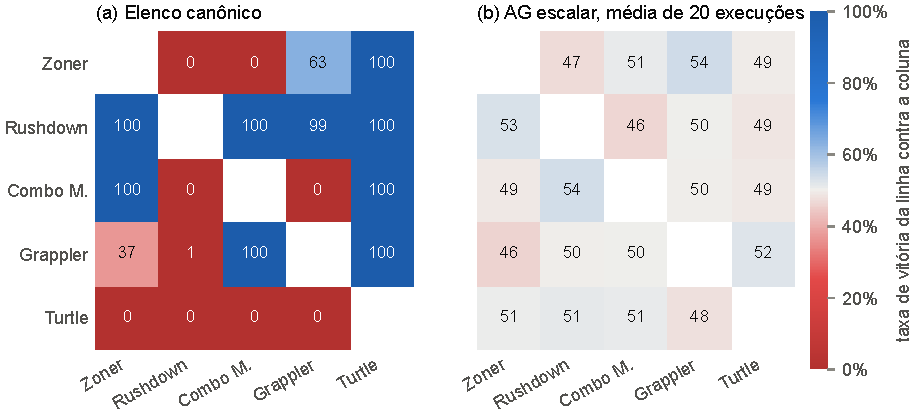
\includegraphics[width=\textwidth]{confrontos.pdf}
    \source
\end{figure}

A \autoref{tab: referencias} traz os valores das métricas no elenco canônico e nos modelos nulos. Três leituras dela orientam o restante do capítulo. A primeira é que o acaso já produz identidade aparente: um elenco sorteado satisfaz em média 5,4 das 18 asserções estruturais e 1,0 das 5 comportamentais, e o melhor dos 30 sorteados em cada régua chega a 9 e a 3. A segunda é que o piso da concordância $\tau$ é de fato zero, mas com dispersão larga: o melhor nulo chega a \nuloTauMelhor{}. A terceira é que nem a simetria perfeita tem $\Pdom$ nulo. Os espelhos, sem identidade alguma, atingem $\Pdom$ médio de \nuloDomEspelho{}, mas a média mistura duas coisas. O espelho do \textit{Zoner} vale \nuloDomEspelhoZoner{}, e \nuloDomEspelhoZonerDecis{} disso vêm do piso de decisividade: as suas lutas são apertadas demais, não desequilibradas. Os outros quatro espelhos ficam entre \nuloDomEspelhosOutros{}. O termo global médio dos cinco, \nuloGlobEspelho{}, é o que o ruído de medição produz num elenco perfeitamente simétrico, e é contra ele, e não contra zero, que o equilíbrio global de um elenco evoluído deve ser lido.

\begin{table}[htb]
    \caption[Métricas do elenco canônico e dos modelos nulos]{Métricas do elenco canônico e dos modelos nulos (1000 lutas por par para $\Pdom$; 200 para as métricas comportamentais). Na última linha, o melhor dos 30 elencos aleatórios em cada coluna, que não é necessariamente o mesmo elenco.}
    \label{tab: referencias}
    \centering
    \small
    % Fonte: results/baselines/baselines.json
    \begin{tabular}{l c c c c c c}
        \toprule
        \textbf{Elenco} & $\Pdom$ & $\Pdrift$ & \textbf{Cam. 1-2} & \textbf{Cam. 3} & $\tau$ & \textbf{Diferenciação} \\
        & & & (de 18) & (de 5) & & \\
        \midrule
        Canônico              & 1,28  & 0     & 18  & 5   & 1       & 1,35 \\
        Espelhos (média)      & 0,033 & 0,377 & 2,6 & 0,6 & $-$0,18 & 0    \\
        Aleatórios (média)    & 1,33  & 0,415 & 5,4 & 1,0 & $-$0,02 & 1,20 \\
        Aleatórios (melhor)   & 1,05  & 0,327 & 9   & 3   & 0,32    & --   \\
        \bottomrule
    \end{tabular}
    \source
\end{table}

\section{Equilíbrio}
\label{sec: res_equilibrio}

\subsection{Convergência}
\label{sub: res_convergencia}

O algoritmo escalar convergiu em todas as 20 execuções, na geração \convGerMediaAG{} $\pm$ \convGerDpAG{} em média, e sempre entre as gerações \convGerMinAG{} e \convGerMaxAG{}. A \autoref{fig: convergencia} mostra a trajetória do melhor elenco de cada geração. O desequilíbrio cai mais de uma ordem de grandeza nas primeiras 30 gerações, de \trajDomIni{} para \trajDomTrinta{} na mediana, e depois oscila em torno de um patamar, como esperado sob a rotação do \textit{stream}: cada geração é avaliada sob sorteios diferentes. O desvio do melhor elenco cai de cerca de 0,4, o valor de um elenco sorteado, para \trajDriftTrinta{} na geração 30, e depois declina devagar até \trajDriftFim{}.

\begin{figure}[htb]
    \caption[Trajetória do melhor elenco de cada geração]{Trajetória do melhor elenco de cada geração, avaliado dentro do laço. Linhas: mediana das 20 execuções; faixas: intervalo interquartil. O híbrido aparece a partir da geração 75, quando começa a sua fase escalar.}
    \label{fig: convergencia}
    \centering
    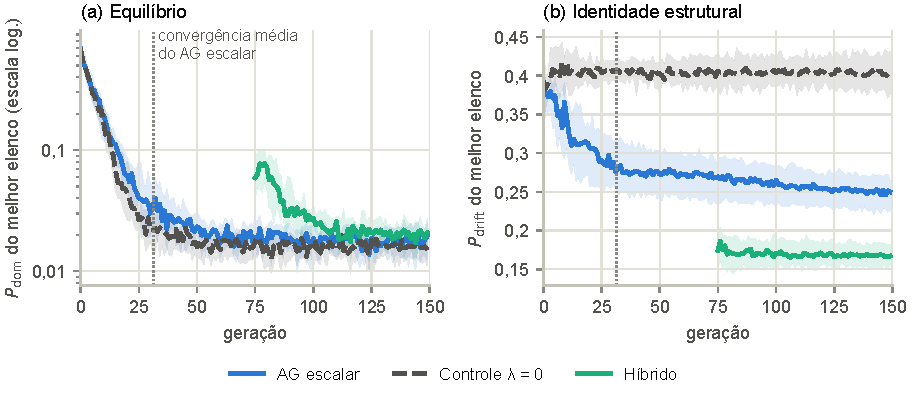
\includegraphics[width=\textwidth]{convergencia.pdf}
    \source
\end{figure}

A confirmação independente foi decisiva. Das \gateDisparosAG{} vezes em que o melhor elenco satisfez o predicado de equilíbrio dentro do laço, \gateRecusasAG{} não sobreviveram à reavaliação num \textit{stream} inédito. Convergir, portanto, marca o primeiro sucesso de um teste repetido a cada geração, e não um estado estável. Ao fim do orçamento, \equilAG{} das 20 execuções terminaram com o elenco equilibrado na reavaliação.

O mesmo fenômeno aparece como degradação entre a avaliação no laço e a reavaliação. O $\Pdom$ do elenco final de cada execução do algoritmo escalar tem mediana \domLacoAG{} no laço e \domAG{} na reavaliação, e a mediana da razão entre os dois é \sobreAG{}. A razão acompanha o peso que a seleção dá ao termo ruidoso. Ela vai de \sobreLzero{} no controle $\lambda_{\mathrm{drift}} = 0$, que só otimiza $\Pdom$, a \sobreNSGA{} no representante \textit{scalar\_optimum} do NSGA-II, em que o desvio é um objetivo separado. Entre os braços que otimizam a mesma soma, ela também varia: \sobreAG{} no algoritmo escalar, \sobreSemSem{} no controle sem semente e \sobreHib{} no híbrido, cuja fase final é escalar. A relação com o peso do termo ruidoso é, portanto, uma tendência, e não uma ordenação exata.

\subsection{Equilíbrio reavaliado}
\label{sub: res_equilibrio_reavaliado}

A \autoref{tab: equilibrio} resume o equilíbrio dos elencos finais de cada braço. Todos os personagens de todas as execuções, em todos os braços, terminaram com taxa de vitória global entre 40\% e 60\%. Equilibrar os personagens globalmente, portanto, não discrimina os métodos. O que discrimina são os pares.

\begin{table}[htb]
    \caption[Equilíbrio dos elencos finais]{Equilíbrio dos elencos finais, reavaliados com 1000 lutas por par. $\Pdom$: mediana e, entre colchetes, primeiro e terceiro quartis; $\tglob$: mediana; $\tcap$ e \textit{hard counters}: média por execução.}
    \label{tab: equilibrio}
    \centering
    \footnotesize
    \setlength{\tabcolsep}{4pt}
    % Fonte: results/multi_run/multi_run_{ga,nsga2}.json e results/controls/multi_run_*.json
    \begin{tabular}{l c c c c c}
        \toprule
        \textbf{Braço} & $\Pdom$ & $\tglob$ & $\tcap$ & \textbf{\textit{Hard counters}} & \textbf{Equilibrados} \\
        \midrule
        AG escalar                      & 0,0355 [0,0252; 0,0418] & 0,0318 & 0,0032 & 0,20 & 16/20 \\
        Híbrido                         & 0,0287 [0,0229; 0,0437] & 0,0287 & 0,0042 & 0,25 & 16/20 \\
        NSGA-II (\textit{scalar\_opt.}) & 0,0759 [0,0492; 0,1031] & 0,0385 & 0,0736 & 2,80 & 0/20 \\
        NSGA-II (\textit{best\_dom.}) & 0,0551 [0,0402; 0,0708] & 0,0378 & 0,0467 & 2,05 & 4/20 \\
        Controle $\lambda_{\mathrm{drift}} = 0$ & 0,0432 [0,0303; 0,0524] & 0,0432 & 0,0000 & 0,05 & 19/20 \\
        Controle sem semente            & 0,0264 [0,0183; 0,0481] & 0,0264 & 0,0016 & 0,10 & 18/20 \\
        \bottomrule
    \end{tabular}
    \source
\end{table}

O algoritmo escalar produz elencos cujo $\Pdom$ mediano, \domAG{}, é da ordem do dos espelhos (\nuloDomEspelho{}), o que o põe na posição de 100\% da \autoref{eq: posicao}, entre o piso dos elencos sem estrutura e a simetria perfeita. Essa posição, porém, é dominada pela distância até o piso (\nuloDomPiso{}) e não distingue o elenco evoluído da simetria. Comparados pelo termo global, que não carrega o piso de decisividade do espelho do \textit{Zoner}, os dois se separam: \globAG{} no algoritmo escalar contra \nuloGlobEspelho{} nos espelhos. Em taxa de vitória, os personagens evoluídos se afastam de 50\% em \desvGlobAGpp{} ponto percentual, na raiz da média dos quadrados, contra \desvGlobEspelhopp{} de puro ruído nos espelhos. O algoritmo escalar chega perto da simetria perfeita, mas não a alcança. A \autoref{fig: confrontos}(b) mostra como esse equilíbrio se distribui: na média das execuções, todos os pares ficam entre 46\% e 54\%. Em execuções individuais, dois pares ultrapassaram a tolerância de \textit{hard counter}, cada um em duas das 20 execuções: \textit{Zoner} contra \textit{Turtle} e \textit{Rushdown} contra \textit{Combo Master}.

O desequilíbrio que resta no NSGA-II é de natureza diferente. O seu termo global é próximo do algoritmo escalar (0,0385 contra 0,0318), mas o termo de \textit{hard counters} é vinte vezes maior (0,0736 contra 0,0032). Os dois equilibram os personagens globalmente de modo parecido; o NSGA-II deixa pares ultrapassarem a tolerância, em média \hcNSGAmedia{} por elenco, e nenhuma das suas 20 execuções termina com o elenco equilibrado.

\subsection{Fora das condições de treino}
\label{sub: res_validacao_externa}

A \autoref{tab: validacao_externa} traz a validação externa dos quatro elencos de semente 42. O elenco do algoritmo escalar é o único que replica: sob sorteios inéditos e 5000 lutas por par, todas as 15 taxas de vitória ficam dentro das faixas de equilíbrio, com $\Pdom = \extDomReplAG{}$, contra \extDomLacoAG{} dentro do laço. O representante \textit{scalar\_optimum} do NSGA-II não replica: o par \textit{Rushdown} contra \textit{Combo Master} fica em 32,7\%, com o intervalo de confiança inteiro fora da faixa. O \textit{knee\_point} e o canônico falham com larga margem.

\begin{table}[htb]
    \caption[Validação externa dos elencos de semente 42]{Validação externa dos elencos de semente 42: veredito (R: robusto; I: inconclusivo; F: frágil) e $\Pdom$ sob cada condição, ambos calculados sobre 5000 lutas por par (10 sementes de 500 lutas, somadas).}
    \label{tab: validacao_externa}
    \centering
    \footnotesize
    \setlength{\tabcolsep}{4pt}
    % Fonte: results/external_validation/external_validation_{evolved,nsga2_scalar_optimum,nsga2_knee_point,canonical}.json
    \begin{tabular}{l c c c c}
        \toprule
        \textbf{Condição} & \textbf{AG escalar} & \textbf{NSGA-II, \textit{scalar\_opt.}} & \textbf{NSGA-II, \textit{knee}} & \textbf{Canônico} \\
        \midrule
        Replicação (regras do treino) & R \; 0,033 & F \; 0,051 & F \; 0,400 & F \; 1,277 \\
        \midrule
        Distância inicial 40        & R \; 0,025 & F \; 0,068 & F \; 0,394 & F \; 1,277 \\
        Distância inicial 60        & R \; 0,040 & F \; 0,045 & F \; 0,396 & F \; 1,278 \\
        Campo 80                    & F \; 0,087 & F \; 0,143 & F \; 0,470 & F \; 1,297 \\
        Campo 120                   & R \; 0,033 & F \; 0,160 & F \; 0,407 & F \; 1,272 \\
        Persistência 4              & I \; 0,110 & F \; 0,273 & F \; 0,440 & F \; 1,283 \\
        Persistência 6              & F \; 0,153 & F \; 0,230 & F \; 0,441 & F \; 1,271 \\
        Multiplicador da guarda 0,55 & I \; 0,075 & F \; 0,108 & F \; 0,397 & F \; 1,277 \\
        Multiplicador da guarda 0,65 & R \; 0,061 & F \; 0,063 & F \; 0,444 & F \; 1,278 \\
        \bottomrule
    \end{tabular}
    \source
\end{table}

Sob regras que a busca nunca viu, o elenco do algoritmo escalar é robusto em quatro das oito condições, inconclusivo em duas e frágil em duas. As falhas se concentram nos pares próximos da borda da faixa. No campo de 80 unidades, o \textit{Zoner} passa a vencer o \textit{Turtle} em 68,8\% das lutas; com persistência 6, o \textit{Combo Master} vence o \textit{Turtle} em 69,4\% e a taxa global do \textit{Turtle} cai a 39,3\%. Nas duas condições inconclusivas, um único par tem o intervalo de confiança cruzando a borda de 35\%. A persistência da intenção é a regra à qual o equilíbrio é mais sensível: as duas perturbações dela produzem os maiores $\Pdom$ da coluna.

\subsection{O que a busca enxerga}
\label{sub: res_sensibilidade}

A \autoref{fig: sensibilidade} mostra a análise de sensibilidade sobre o elenco do algoritmo escalar de semente 42. O alcance, o dano, o intervalo entre golpes e os pontos de vida movem a taxa de vitória com força: deslocar o alcance numa janela de um desvio de mutação para cada lado muda a taxa global dos personagens em 30,8 pontos percentuais em média, contra um piso de ruído medido de \sensPiso{} pontos. O agarrão e o atordoamento também são claramente visíveis. O peso de RECUAR, a repulsão e a velocidade ficam na faixa limítrofe, e os pesos de FRENTE e de GUARDA, no fundo da ordenação, não se distinguem do ruído. A janela dos pesos comportamentais, porém, é quatro vezes mais estreita que a dos atributos, porque o desvio da mutação deles é menor (\autoref{sec: ag_escalar}).

\begin{figure}[htb]
    \caption[Sensibilidade de cada gene no elenco do algoritmo escalar]{Sensibilidade de cada gene no elenco do algoritmo escalar de semente 42: variação média absoluta da taxa de vitória global dos cinco personagens numa janela de dois desvios-padrão de mutação.}
    \label{fig: sensibilidade}
    \centering
    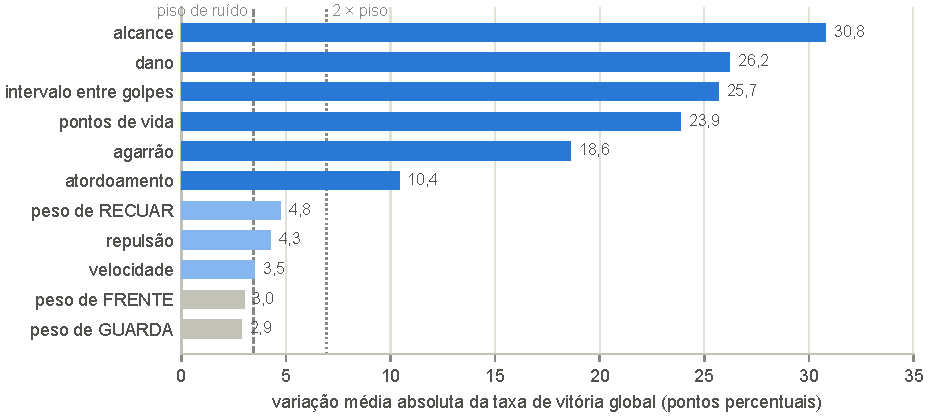
\includegraphics[width=\textwidth]{sensibilidade.pdf}
    \source
\end{figure}

A diferença de janela separa duas explicações para o fundo da ordenação: a política pesar pouco no combate, ou a mutação mexer pouco nela. Numa medição feita para este texto, os pesos foram deslocados com a mesma janela relativa dos atributos, de 10\% da amplitude para cada lado. Nessa condição, os três pesos movem a taxa global em \sensPesosIguais{} pontos percentuais (\sensWRIgual{} no de RECUAR, \sensWFIgual{} no de FRENTE e \sensWGIgual{} no de GUARDA), acima do atordoamento (\sensStun{}), da repulsão (\sensKb{}) e da velocidade (\sensSpd{}). A política pesa no combate tanto quanto os atributos intermediários. O que a esconde da busca é o passo com que a mutação a altera: nesse passo, o efeito de cada mutação sobre o equilíbrio fica no nível do ruído, e o único termo da aptidão que ainda distingue uma mutação de outra é o de identidade. Essa assimetria reaparece na \autoref{sub: res_perdas}.

\section{Identidade}
\label{sec: res_identidade}

\subsection{Identidade do algoritmo escalar}
\label{sub: res_identidade_ag}

A \autoref{fig: metricas} mostra a distribuição, nas 20 execuções de cada braço, das seis métricas da família de testes. Tomado isoladamente, o algoritmo escalar preserva a identidade estrutural com folga sobre o acaso: desvio mediano de \driftAG{}, contra 0,415 dos elencos sorteados, e \LumdoisAG{} das 18 asserções das Camadas 1 e 2, contra 5,4 em média e 9 no melhor nulo. Essa régua, contudo, é parcialmente endógena, e superar os nulos nela é esperado de qualquer busca com o termo de desvio.

\begin{figure}[htbp]
    \caption[As seis métricas da família de testes por braço]{As seis métricas da família de testes nas 20 execuções de cada braço. Pontos: execuções; barra preta: mediana. Linha tracejada: média dos espelhos em (a) e dos elencos aleatórios de (c) a (f). O NSGA-II aparece pelo representante \textit{scalar\_optimum}.}
    \label{fig: metricas}
    \centering
    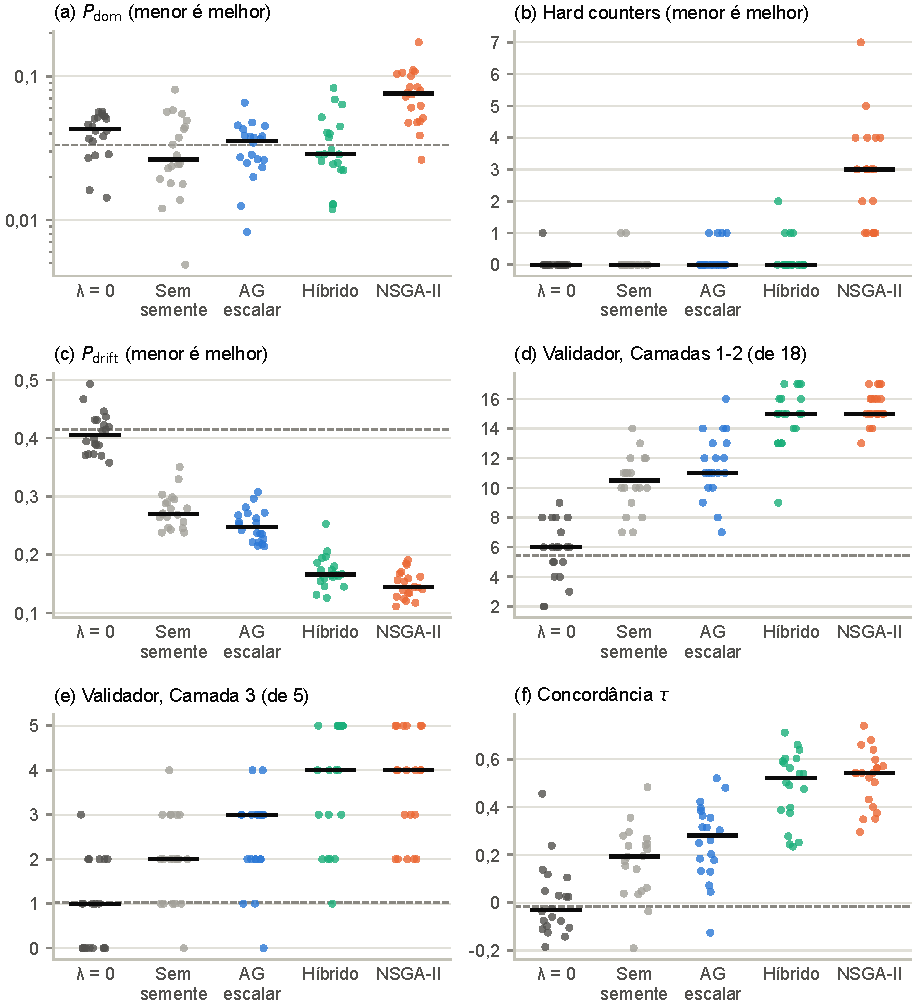
\includegraphics[width=\textwidth]{metricas.pdf}
    \source
\end{figure}

A identidade funcional é mais modesta. A mediana é de \LtresAG{} das 5 asserções comportamentais e $\tau = \tauAG{}$. Os dois valores estão acima da média dos elencos sorteados (1,0 e $-0{,}02$), mas no topo da distribuição dos nulos: o melhor elenco sorteado também atinge 3 asserções comportamentais e $\tau = \nuloTauMelhor{}$. Um elenco evoluído isolado, comparado a 35 nulos, não tem resolução para concluir. O elenco de semente 42, por exemplo, empata com o melhor nulo na Camada 3 ($p = 0{,}03$) e fica um fio abaixo dele na concordância ($\tau = 0{,}314$, $p = 0{,}06$). A evidência sobre a identidade funcional vem, por isso, da comparação com o controle.

\subsection{O contrafactual: equilibrar sem o termo de identidade}
\label{sub: res_controle}

A \autoref{tab: controles} compara o algoritmo escalar com os dois braços de controle. Sem o termo de identidade, o mesmo algoritmo, com a mesma amostra e o mesmo orçamento, perde a identidade nas quatro réguas, todas com efeito grande e $p_{\mathrm{Holm}} \le \pHolmLzeroIdentMax{}$. O desvio mediano sobe de \driftAG{} para \driftLzero{}; as asserções estruturais caem de \LumdoisAG{} para \LumdoisLzero{}; as comportamentais, de \LtresAG{} para \LtresLzero{}; e a concordância cai de \tauAG{} para \tauLzero{}, com média de \tauLzeroMedia{} nas 20 execuções.

\begin{table}[htb]
    \caption[Algoritmo escalar contra os dois controles]{Algoritmo escalar contra os dois controles: medianas, $p$ corrigido por Holm (Wilcoxon pareado) e $\hat{A}_{12}$ (probabilidade de o AG escalar dar valor maior).}
    \label{tab: controles}
    \centering
    \small
    % Fonte: results/controls/comparison_ga_vs_ga_drift0_dom1.json e comparison_ga_vs_ga_unseeded.json
    \begin{tabular}{l c c c c c c c}
        \toprule
        & & \multicolumn{3}{c}{\textbf{Controle $\lambda_{\mathrm{drift}} = 0$}} & \multicolumn{3}{c}{\textbf{Controle sem semente}} \\
        \cmidrule(lr){3-5} \cmidrule(lr){6-8}
        \textbf{Métrica} & \textbf{AG} & \textbf{Med.} & $p_{\mathrm{Holm}}$ & $\hat{A}_{12}$ & \textbf{Med.} & $p_{\mathrm{Holm}}$ & $\hat{A}_{12}$ \\
        \midrule
        $\Pdom$              & 0,0355 & 0,0432  & 0,059                & 0,30 & 0,0264 & 0,99   & 0,55 \\
        \textit{Hard counters} & 0    & 0       & 0,18                 & 0,57 & 0      & 0,83   & 0,55 \\
        $\Pdrift$            & 0,2473 & 0,4055  & $1{,}1\cdot10^{-5}$  & 0,00 & 0,2703 & 0,0073 & 0,25 \\
        Camadas 1-2          & 11     & 6       & $4{,}2\cdot10^{-4}$  & 0,98 & 10,5   & 0,31   & 0,66 \\
        Camada 3             & 3      & 1       & 0,0044               & 0,85 & 2      & 0,59   & 0,64 \\
        $\tau$               & 0,28   & $-$0,03 & $6{,}7\cdot10^{-4}$  & 0,87 & 0,19   & 0,39   & 0,67 \\
        \bottomrule
    \end{tabular}
    \source
\end{table}

O controle não perde apenas \textit{parte} da identidade: ele cai ao nível do acaso. O seu desvio (\driftLzero{}) é o de um elenco sorteado (0,415); as suas asserções estruturais (6) e comportamentais (1) estão na média dos elencos sorteados; a sua concordância média, \tauLzeroMedia{}, é a do acaso. A \autoref{fig: metricas} mostra o mesmo em cada execução: nas quatro réguas de identidade, a nuvem do controle fica sobre a linha dos elencos aleatórios. Sem o termo de identidade, o equilíbrio é alcançado com elencos que não guardam relação com os arquétipos.

No equilíbrio, os dois braços não se separam. O $\Pdom$ mediano do controle é maior (\domLzero{} contra \domAG{}), com efeito médio ($\hat{A}_{12} = \aLzeroDom{}$) e $p$ bruto de \pBrutoLzeroDom{}, mas a diferença não sobrevive à correção para múltiplas comparações ($p_{\mathrm{Holm}} = \pHolmLzeroDom{}$). O número de \textit{hard counters} também não separa. E, descritivamente, o controle termina equilibrado em \equilLzero{} das 20 execuções, contra \equilAG{} do algoritmo escalar. O resultado sustenta que a identidade não custou equilíbrio mensurável. Não sustenta que ela o melhore.

O controle sem a semente canônica separa do algoritmo escalar apenas no desvio (\driftSemSem{} contra \driftAG{}, $p_{\mathrm{Holm}} = \pHolmSemSemDrift{}$), e em nenhuma outra métrica. Nas demais réguas de identidade, as estimativas também favorecem a semente, com efeito médio nas Camadas 1 e 2 e na concordância $\tau$ (\autoref{tab: controles}), mas sem significância. A semente contribui um pouco para a identidade e não explica as diferenças entre o algoritmo escalar e o NSGA-II relatadas na \autoref{sec: res_compromisso}.

\subsection{O que se preserva e o que se perde}
\label{sub: res_perdas}

A \autoref{tab: assercoes} desagrega o validador: em quantas das 20 execuções de cada braço cada asserção foi satisfeita. Três padrões aparecem.

\begin{table}[htbp]
    \caption[Asserções do validador satisfeitas por braço]{Número de execuções, em 20, em que cada asserção do validador foi satisfeita. Para as asserções das Camadas 1 e 3, o acaso dá em torno de 4 em 20. O NSGA-II aparece pelo representante \textit{scalar\_optimum}.}
    \label{tab: assercoes}
    \centering
    \footnotesize
    % Fonte: validador reaplicado aos genes gravados em results/multi_run e results/controls
    % (200 lutas por par, semente 9999); reproduz os totais gravados nas 80 execuções.
    \begin{tabularx}{\textwidth}{l X c c c c}
        \toprule
        \textbf{Arquétipo} & \textbf{Asserção} & \textbf{AG} & \textbf{Híbrido} & \textbf{NSGA-II} & $\boldsymbol{\lambda = 0}$ \\
        \midrule
        \multicolumn{6}{l}{\textit{Camada 1: genes, entre personagens}} \\
        \textit{Rushdown}     & maior velocidade                     & 16 & 19 & 17 & 3 \\
                              & menor intervalo entre golpes         & 16 & 19 & 19 & 8 \\
                              & maior probabilidade de FRENTE        & 5  & 4  & 5  & 4 \\
        \textit{Zoner}        & maior alcance                        & 11 & 16 & 17 & 4 \\
                              & maior repulsão                       & 12 & 14 & 18 & 5 \\
                              & maior probabilidade de RECUAR        & 9  & 15 & 17 & 6 \\
        \textit{Combo Master} & maior atordoamento                   & 16 & 18 & 18 & 2 \\
        \textit{Grappler}     & maior dano                           & 10 & 19 & 19 & 4 \\
                              & maior poder de agarrão               & 16 & 18 & 19 & 4 \\
        \textit{Turtle}       & menor velocidade                     & 12 & 16 & 17 & 5 \\
                              & maior intervalo entre golpes         & 9  & 13 & 15 & 4 \\
                              & mais pontos de vida                  & 10 & 19 & 20 & 4 \\
                              & maior probabilidade de GUARDA        & 10 & 15 & 16 & 2 \\
        \midrule
        \multicolumn{6}{l}{\textit{Camada 2: genes, no mesmo personagem}} \\
        \textit{Zoner}        & alcance maior que velocidade         & 15 & 19 & 19 & 8 \\
        \textit{Rushdown}     & velocidade maior que alcance         & 20 & 20 & 20 & 16 \\
        \textit{Grappler}     & pontos de vida maiores que velocidade & 11 & 18 & 19 & 7 \\
        \textit{Combo Master} & atordoamento maior que repulsão      & 18 & 20 & 20 & 13 \\
                              & velocidade maior que alcance         & 14 & 13 & 14 & 15 \\
        \midrule
        \multicolumn{6}{l}{\textit{Camada 3: comportamento}} \\
        \textit{Zoner}        & maior distância média de luta        & 10 & 16 & 17 & 2 \\
        \textit{Rushdown}     & mais golpes conectados               & 3  & 10 & 11 & 6 \\
        \textit{Turtle}       & maior fração de defesa escolhida     & 11 & 15 & 16 & 2 \\
        \textit{Combo Master} & maior atordoamento infligido         & 12 & 16 & 14 & 3 \\
        \textit{Grappler}     & maior dano através da guarda         & 13 & 17 & 15 & 5 \\
        \bottomrule
    \end{tabularx}
    \source
\end{table}

O primeiro padrão é que o controle $\lambda_{\mathrm{drift}} = 0$ fica no nível do acaso asserção por asserção, e não apenas no total. O segundo é que o algoritmo escalar preserva melhor os traços de ritmo do \textit{Rushdown} (velocidade e intervalo entre golpes), o atordoamento do \textit{Combo Master} e o agarrão do \textit{Grappler}, todos em 16 de 20 execuções, e perde mais os traços do \textit{Zoner} e do \textit{Turtle}, que ficam entre 9 e 12. O terceiro, e o mais nítido, é que a asserção da política do \textit{Rushdown}, ser o personagem de maior probabilidade de avançar, é satisfeita em apenas 4 a 5 de 20 execuções em \textit{todos} os braços, inclusive nos que melhor preservam a identidade. Em boa parte dessas falhas, o \textit{Combo Master}, cuja probabilidade canônica de FRENTE (0,74) já é próxima da do \textit{Rushdown}, passa a avançar mais que ele. Isso ocorre em \cmAvancaMaisAG{} das 20 execuções do algoritmo escalar, em \cmAvancaMaisNSGA{} das do NSGA-II e em \cmAvancaMaisHib{} das do híbrido. A asserção comportamental correspondente, ser o que mais golpeia, cai para 3 em 20 no algoritmo escalar.

A \autoref{tab: politica} mostra a origem desse padrão. Ela compara, para cada arquétipo, a probabilidade da intenção que o define no elenco canônico com a mediana dessa probabilidade nas execuções de cada braço. Nos elencos evoluídos, a política de todos os personagens se afasta do perfil canônico, mas não em direção a uma política sorteada ao acaso, que daria 1/3 a cada intenção. Os personagens se aproximam de um perfil comum, que recua pouco: no algoritmo escalar, os quatro arquétipos além do \textit{Zoner} recuam em \polAGRecuoOutros{} das intenções. O \textit{Rushdown} canônico avança em 86\% das intenções; o do algoritmo escalar, em 39\%, e o do NSGA-II, em 48\%. No controle sem termo de identidade, as políticas dos cinco arquétipos são praticamente indistinguíveis entre si: na mediana, todos avançam em \polLzeroF{} das intenções, recuam em \polLzeroR{} e guardam em \polLzeroG{}. O valor baixo do \textit{Zoner} na \autoref{tab: politica} não o distingue: é a propensão a recuar comum aos cinco.

\begin{table}[htb]
    \caption[Probabilidade da intenção que define cada arquétipo]{Probabilidade da intenção que define cada arquétipo: valor canônico e mediana das 20 execuções de cada braço. Uma política sorteada ao acaso dá, em média, 1/3 a cada intenção. O NSGA-II aparece pelo representante \textit{scalar\_optimum}.}
    \label{tab: politica}
    \centering
    \small
    % Fonte: genes gravados em results/multi_run e results/controls (probabilidades da Eq. de intenção)
    \begin{tabular}{l l c c c c c}
        \toprule
        \textbf{Arquétipo} & \textbf{Intenção} & \textbf{Canônico} & \textbf{AG} & \textbf{Híbrido} & \textbf{NSGA-II} & $\boldsymbol{\lambda = 0}$ \\
        \midrule
        \textit{Rushdown}     & FRENTE & 0,86 & 0,39 & 0,47 & 0,48 & 0,35 \\
        \textit{Combo Master} & FRENTE & 0,74 & 0,47 & 0,51 & 0,55 & 0,40 \\
        \textit{Grappler}     & FRENTE & 0,58 & 0,41 & 0,44 & 0,44 & 0,36 \\
        \textit{Zoner}        & RECUAR & 0,55 & 0,33 & 0,45 & 0,46 & 0,19 \\
        \textit{Turtle}       & GUARDA & 0,54 & 0,45 & 0,47 & 0,48 & 0,40 \\
        \bottomrule
    \end{tabular}
    \source
\end{table}

A diferenciação, calculada para este texto a partir dos genes gravados, não acrescenta evidência. Ela cai de \difCanon{} no canônico para \difAG{} na mediana do algoritmo escalar, abaixo da média dos elencos sorteados (\difAleat{}), enquanto o híbrido (\difHib{}) e o NSGA-II (\difNSGA{}) ficam no nível dos sorteados. O controle sem termo de identidade, porém, fica em \difLzero{}, acima do algoritmo escalar. Se o equilíbrio fosse o que aproxima os personagens, o braço que só otimiza equilíbrio teria o menor valor. Como elencos sorteados são dispersos sem ter identidade alguma, a métrica não separa identidade de dispersão, e não serve como evidência de homogeneização pelo equilíbrio.

\section{O compromisso entre equilíbrio e identidade}
\label{sec: res_compromisso}

\subsection{A fronteira de Pareto}
\label{sub: res_fronteira}

A \autoref{fig: fronteira} sobrepõe as 20 fronteiras finais do NSGA-II e os elencos finais dos braços escalares, todos avaliados dentro do laço, sob o \textit{stream} da última geração de cada semente. As fronteiras têm em média \fronteiraTamMedio{} pontos e são notavelmente estáveis entre execuções: o hipervolume é \hvMedia{} $\pm$ \hvDp{} e o espaçamento, \espacMedia{} $\pm$ \espacDp{}. O formato é o de um compromisso íngreme. Na ponta de identidade, os elencos mantêm desvio próximo de 0,06, mas com $\Pdom$ acima de 1, tão desequilibrados quanto o canônico. Para reduzir $\Pdom$ a um décimo desse valor, a fronteira paga de 0,08 a 0,1 em desvio.

\begin{figure}[htb]
    \caption[Fronteiras finais do NSGA-II e elencos finais dos demais braços]{Fronteiras finais do NSGA-II (20 execuções) e elencos finais dos demais braços, todos avaliados dentro do laço, sob o \textit{stream} da última geração. O elenco canônico aparece pela sua reavaliação com 1000 lutas por par.}
    \label{fig: fronteira}
    \centering
    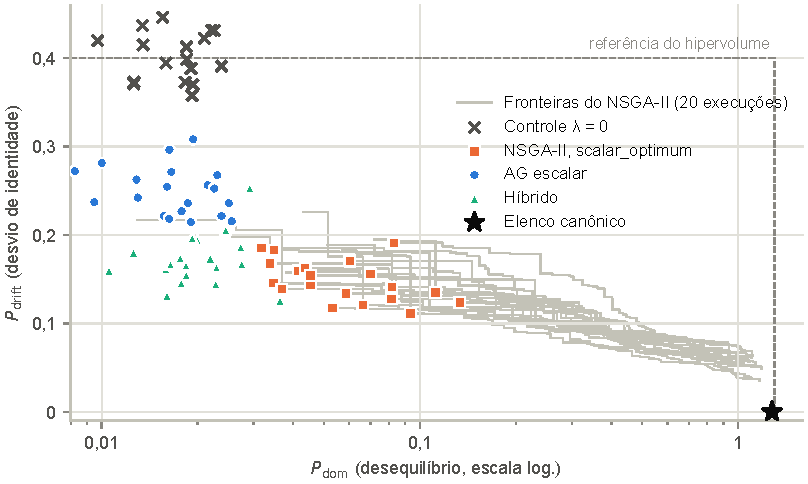
\includegraphics[width=\textwidth]{fronteira.pdf}
    \source
\end{figure}

A \autoref{tab: representantes} resume os cinco representantes extraídos de cada fronteira. Os três pontos geométricos, o extremo de identidade, o joelho e o ideal, preservam quase toda a identidade (Camada 3 em 5 de 5, $\tau$ de 0,70 a 0,80), mas nenhum deles termina equilibrado em nenhuma execução. Os pontos de interesse para a pergunta de pesquisa estão na ponta de equilíbrio da fronteira.

\begin{table}[htb]
    \caption[Representantes das fronteiras do NSGA-II]{Representantes das fronteiras do NSGA-II, reavaliados: medianas das 20 execuções; \textit{hard counters} em média por execução.}
    \label{tab: representantes}
    \centering
    \small
    % Fonte: results/multi_run/multi_run_nsga2.json (representatives)
    \begin{tabular}{l c c c c c c c}
        \toprule
        \textbf{Representante} & $\Pdom$ & $\Pdrift$ & \textbf{\textit{H. c.}} & \textbf{Equil.} & \textbf{Cam. 1-2} & \textbf{Cam. 3} & $\tau$ \\
        \midrule
        \textit{best\_drift}     & 1,056 & 0,059 & 8,45 & 0/20 & 18   & 5 & 0,80 \\
        \textit{knee\_point}     & 0,405 & 0,087 & 6,85 & 0/20 & 17   & 5 & 0,70 \\
        \textit{ideal\_point}    & 0,396 & 0,087 & 7,25 & 0/20 & 17,5 & 5 & 0,71 \\
        \textit{scalar\_optimum} & 0,076 & 0,145 & 2,80 & 0/20 & 15   & 4 & 0,54 \\
        \textit{best\_dominance} & 0,055 & 0,166 & 2,05 & 4/20 & 15   & 4 & 0,51 \\
        \bottomrule
    \end{tabular}
    \source
\end{table}

\subsection{Algoritmo escalar e NSGA-II}
\label{sub: res_ag_nsga}

A \autoref{tab: comparacoes} traz a comparação estatística do algoritmo escalar com o NSGA-II e com o híbrido. Contra o \textit{scalar\_optimum}, as seis métricas da família são significativas, todas com efeito grande ($p_{\mathrm{Holm}} \le \pHolmNSGAmax{}$), e a divisão é limpa. O algoritmo escalar vence as duas métricas de equilíbrio: $\Pdom$ de \domAG{} contra \domNSGA{} e nenhum \textit{hard counter} na mediana, contra 3. O NSGA-II vence as quatro de identidade: desvio de \driftNSGA{} contra \driftAG{}, com separação completa ($\hat{A}_{12} = 1{,}00$), \LumdoisNSGA{} asserções estruturais contra \LumdoisAG{}, \LtresNSGA{} comportamentais contra \LtresAG{} e concordância de \tauNSGA{} contra \tauAG{}. Contra o extremo \textit{best\_dominance}, as seis diferenças mantêm a direção e a significância, com efeitos um pouco menores em equilíbrio. Em todas as comparações, o número de personagens em banda foi constante (5 em todas as execuções) e ficou fora da família de testes, que teve seis métricas.

\begin{table}[htb]
    \caption[Algoritmo escalar contra o NSGA-II e o híbrido]{Algoritmo escalar contra o NSGA-II e o híbrido: medianas, $p$ corrigido por Holm (Wilcoxon pareado) e $\hat{A}_{12}$ (probabilidade de o AG escalar dar valor maior). Todos os efeitos com $p_{\mathrm{Holm}} < 0{,}05$ são grandes.}
    \label{tab: comparacoes}
    \centering
    \footnotesize
    \setlength{\tabcolsep}{4pt}
    % Fonte: results/multi_run/comparison_ga_vs_nsga2*.json e results/controls/comparison_ga_vs_hybrid_split0.5_front.json
    \begin{tabular}{l c ccc ccc ccc}
        \toprule
        & & \multicolumn{3}{c}{\textbf{NSGA-II, \textit{scalar\_opt.}}} & \multicolumn{3}{c}{\textbf{NSGA-II, \textit{best\_dom.}}} & \multicolumn{3}{c}{\textbf{Híbrido}} \\
        \cmidrule(lr){3-5} \cmidrule(lr){6-8} \cmidrule(lr){9-11}
        \textbf{Métrica} & \textbf{AG} & \textbf{Med.} & $p_{\mathrm{Holm}}$ & $\hat{A}_{12}$ & \textbf{Med.} & $p_{\mathrm{Holm}}$ & $\hat{A}_{12}$ & \textbf{Med.} & $p_{\mathrm{Holm}}$ & $\hat{A}_{12}$ \\
        \midrule
        $\Pdom$                & 0,0355 & 0,0759 & $9{,}5\cdot10^{-5}$ & 0,07 & 0,0551 & 0,0034              & 0,18 & 0,0287 & 1,00                & 0,51 \\
        \textit{Hard counters} & 0      & 3      & $3{,}4\cdot10^{-4}$ & 0,03 & 2      & 0,0021              & 0,14 & 0      & 1,00                & 0,49 \\
        $\Pdrift$              & 0,2473 & 0,1445 & $1{,}1\cdot10^{-5}$ & 1,00 & 0,1663 & $2{,}3\cdot10^{-5}$ & 0,98 & 0,1663 & $1{,}1\cdot10^{-5}$ & 0,97 \\
        Camadas 1-2            & 11     & 15     & $3{,}4\cdot10^{-4}$ & 0,05 & 15     & 0,0013              & 0,09 & 15     & 0,0026              & 0,12 \\
        Camada 3               & 3      & 4      & 0,0027              & 0,24 & 4      & 0,0034              & 0,24 & 4      & 0,0058              & 0,24 \\
        $\tau$                 & 0,28   & 0,54   & $1{,}1\cdot10^{-4}$ & 0,09 & 0,51   & $5{,}2\cdot10^{-4}$ & 0,13 & 0,52   & $8{,}4\cdot10^{-4}$ & 0,15 \\
        \bottomrule
    \end{tabular}
    \source
\end{table}

Nenhuma dessas conclusões depende da escolha do teste. O teste não pareado de Mann-Whitney, reportado ao lado nos artefatos, dá $p$ brutos menores que 0,004 nas seis métricas da comparação com o \textit{scalar\_optimum}.

\subsection{Relação de Pareto por semente}
\label{sub: res_pareto}

A comparação por representante mede, em parte, a escolha do representante. A relação de Pareto por semente não depende dela. Em 18 das 20 sementes, o ponto do algoritmo escalar e a fronteira do NSGA-II são mutuamente não dominados; em uma, o ponto do escalar domina algum ponto da fronteira; e em outra, é dominado por ela. A \autoref{fig: fronteira} mostra por quê: em 19 das 20 sementes, o ponto do algoritmo escalar está \textit{além} da ponta de equilíbrio da fronteira, com $\Pdom$ no laço de \domLacoAG{} contra \domLacoFronteiraMin{} no ponto mais equilibrado da fronteira. O escalar alcança um equilíbrio que a fronteira não oferece, pagando em desvio.

Ser não dominado, contudo, não é ser ótimo na própria função. Na soma $\Pdom + \Pdrift$, que é exatamente o que o algoritmo escalar maximiza com sinal trocado (\autoref{eq: aptidao_escalar}), a fronteira do NSGA-II contém um ponto melhor que o do escalar em 20 das 20 sementes, com medianas de \somaFronteira{} contra \somaAG{} dentro do laço. A avaliação no laço favorece mais o algoritmo escalar que o NSGA-II (\autoref{sub: res_convergencia}), e a conclusão se mantém com os elencos reavaliados: o representante \textit{scalar\_optimum} tem soma menor que a do escalar em \somaReavSOmelhorAG{} das 20 sementes. O algoritmo escalar termina num extremo do compromisso, e não no ponto que a sua própria função de aptidão preferiria.

\subsection{O híbrido}
\label{sub: res_hibrido}

A última coluna da \autoref{tab: comparacoes} compara o híbrido com o algoritmo escalar. As duas métricas de equilíbrio não se movem: $\hat{A}_{12}$ de 0,51 e 0,49, $p_{\mathrm{Holm}} = 1{,}00$, e \equilHib{} elencos equilibrados em 20, como no escalar. As quatro métricas de identidade melhoram, todas com efeito grande e $p_{\mathrm{Holm}} \le \pHolmHibIdentMax{}$: o desvio cai de \driftAG{} para \driftHib{}; as asserções estruturais sobem de \LumdoisAG{} para \LumdoisHib{} e as comportamentais, de \LtresAG{} para \LtresHib{}; a concordância quase dobra, de \tauAG{} para \tauHib{}.

Descritivamente, o híbrido reúne a metade favorável de cada algoritmo. A sua identidade fica próxima da do NSGA-II (desvio \driftHib{} contra \driftNSGA{}, concordância \tauHib{} contra \tauNSGA{}, Camada 3 igual), com o equilíbrio do algoritmo escalar: 0,25 \textit{hard counters} por elenco contra \hcNSGAmedia{}, e \equilHib{} elencos equilibrados contra \equilNSGA{}. Na \autoref{fig: fronteira}, os pontos do híbrido ficam, como os do algoritmo escalar, à esquerda da ponta de equilíbrio das fronteiras (em \hibAlemPonta{} das 20 sementes), mas com desvio menor que o deles. Em nenhuma semente o ponto do híbrido é dominado pela fronteira do NSGA-II da mesma semente, e em \hibDominaFronteira{} das 20 ele domina algum ponto dela. Ao contrário do algoritmo escalar, o híbrido termina perto do ótimo da própria função. A fronteira contém um ponto de soma $\Pdom + \Pdrift$ menor que a dele em apenas \hibFronteiraMelhor{} das 20 sementes, contra 20 de 20 no escalar, e a mediana da sua soma no laço, \somaHib{}, fica abaixo da do melhor ponto da fronteira, \somaFronteira{}. Com os elencos reavaliados, o híbrido tem soma menor que a do representante \textit{scalar\_optimum} em \somaReavHibMelhorSO{} das 20 sementes. Essa comparação com o NSGA-II é descritiva: a família de testes pré-definida opõe o algoritmo escalar a cada braço, e não os braços entre si.

O preço do híbrido é a velocidade. Ele converge, em média, na geração \convGerMediaHib{} $\pm$ \convGerDpHib{}, contra \convGerMediaAG{} $\pm$ \convGerDpAG{} do escalar, porque as suas primeiras 75 gerações são de Pareto e não perseguem o predicado de equilíbrio. A \autoref{fig: convergencia} mostra a consequência: ao receber a fronteira, a fase escalar parte de um $\Pdom$ mais alto que o do escalar na mesma geração, aproxima-se dele nas gerações seguintes e mantém o desvio no nível do NSGA-II até o fim.

\section{Estrutura de vantagens}
\label{sec: res_ciclo}

A \autoref{tab: ciclo} resume o teste do ciclo autoral, com 16\,000 lutas por par.

\begin{table}[htb]
    \caption[Teste do ciclo autoral de vantagens]{Teste do ciclo autoral de vantagens (16\,000 lutas por par): arestas decididas por elenco, arestas mantidas entre as decididas, tríades circulares e margem mediana das arestas de cada elenco, em média sobre os elencos. O NSGA-II aparece pelo representante \textit{scalar\_optimum}.}
    \label{tab: ciclo}
    \centering
    \small
    % Fonte: results/cycle/cycle_structure.json
    \begin{tabular}{l c c c c c}
        \toprule
        \textbf{Grupo} & \textbf{Elencos} & \textbf{Decididas} & \textbf{Mantidas} & \textbf{Tríades} & \textbf{Margem} \\
        & & (de 10) & (das decididas) & (de 5) & \\
        \midrule
        Canônico    & 1  & 10,00 & 6/10 (60\%)        & 1,00 & 0,500 \\
        AG escalar  & 20 & 9,30  & 105/186 (56,5\%)   & 3,71 & 0,048 \\
        NSGA-II     & 20 & 9,85  & 98/197 (49,7\%)    & 4,17 & 0,104 \\
        Espelhos    & 5  & 1,00  & 3/5                & 2,59 & 0,003 \\
        Aleatórios  & 30 & 10,00 & 149/300 (49,7\%)   & 0,40 & 0,491 \\
        \bottomrule
    \end{tabular}
    \source
\end{table}

O primeiro resultado é sobre o próprio canônico: ele realiza apenas 6 das 10 arestas autorais. As quatro que quebra são inversões completas: o \textit{Combo Master} vence o \textit{Grappler} em 0,2\% das lutas, e não na maioria; o \textit{Grappler} vence o \textit{Rushdown} em 0,6\%; e o \textit{Turtle} não vence nem o \textit{Rushdown} nem o \textit{Combo Master}. Lidas juntas com a \autoref{fig: confrontos}(a), essas arestas descrevem uma hierarquia, e não um ciclo: o \textit{Rushdown} vence todos e o \textit{Turtle} perde para todos. As tríades circulares confirmam, com \triadesCanon{} de um máximo de 5.

Nos elencos evoluídos, o ciclo não é realizado. O algoritmo escalar mantém \cicloMantidasAG{} das \cicloDecididasAG{} arestas decididas, \cicloTaxaAG{}, uma inclinação na direção autoral que não é significativa: $p = \cicloBinomAG{}$ no teste binomial, e $p = \cicloPNulos{}$ ($\hat{A}_{12} = \cicloANulos{}$) contra os elencos aleatórios, que ficam em \cicloTaxaNulos{}. O NSGA-II mantém praticamente metade. A aresta mais emblemática, o agarrão do \textit{Grappler} contra a guarda do \textit{Turtle}, vence 100\% das lutas no canônico e fica em 52\% na média das execuções do algoritmo escalar.

As tríades mostram onde está a estrutura não transitiva. Elas são quase nulas nos elencos aleatórios (\triadesAleat{}), mínimas no canônico (\triadesCanon{}) e altas nos elencos evoluídos: \triadesAG{} no algoritmo escalar e \triadesNSGA{} no NSGA-II, com quase todas as arestas decididas. Os espelhos, com \triadesEspelho{} tríades e apenas uma aresta decidida por elenco, mostram que a contagem só tem significado quando as arestas são decididas.

\section{Síntese}
\label{sec: res_sintese}

O \autoref{quad: sintese} reúne as respostas às três questões de pesquisa, na forma mais estreita que os dados sustentam.

\begin{quadro}[htb]
    \caption{Respostas às questões de pesquisa.}
    \label{quad: sintese}
    \centering
    \small
    \begin{tabularx}{\textwidth}{l X}
        \toprule
        \textbf{Questão} & \textbf{Resposta} \\
        \midrule
        QP1: equilíbrio & Sim. O algoritmo escalar converge em todas as execuções e termina, na mediana, perto da simetria perfeita, com o elenco equilibrado em 16 de 20. O elenco da semente 42, único submetido à validação externa, replica fora do laço e é robusto a 4 de 8 regras não vistas, frágil em 2. \\
        \midrule
        QP2: identidade & Parcialmente, e a parte preservada é atribuível ao termo de identidade. Sem ele, a identidade cai ao nível do acaso nas quatro réguas, sem ganho de equilíbrio significativo. Com ele, a identidade funcional fica acima do acaso, mas longe do canônico, e a política dos personagens é o componente menos preservado. \\
        \midrule
        QP3: compromisso & O algoritmo escalar ocupa a ponta de equilíbrio do compromisso, além da fronteira do NSGA-II; o NSGA-II preserva mais identidade e deixa pares desequilibrados. Nenhum domina o outro. O híbrido, com o mesmo orçamento, aproxima-se da identidade do NSGA-II mantendo o equilíbrio do escalar. \\
        \bottomrule
    \end{tabularx}
    \source
\end{quadro}

  \chapter[Discussão]{Discussão}
\label{chap: discussao}

Este capítulo interpreta os resultados do \autoref{chap: resultados}. A \autoref{sec: disc_resposta} responde à pergunta de pesquisa. As seções seguintes discutem os quatro achados que qualificam essa resposta: o termo de identidade como penalidade que pode perder (\autoref{sec: disc_penalidade}), a política como o componente de identidade menos preservado (\autoref{sec: disc_politica}), o efeito do ruído de avaliação sobre a seleção escalar (\autoref{sec: disc_ruido}) e o ciclo de vantagens que o modelo não realiza (\autoref{sec: disc_ciclo}). A \autoref{sec: disc_medicao} reúne as lições de método, a \autoref{sec: disc_robustez} discute a robustez do equilíbrio, e a \autoref{sec: limitacoes} delimita o alcance das conclusões.

\section{Resposta à pergunta de pesquisa}
\label{sec: disc_resposta}

A pergunta era se um algoritmo genético consegue atingir equilíbrio competitivo entre cinco arquétipos sem destruir suas identidades funcionais. A resposta que os dados sustentam é afirmativa, com uma qualificação sobre \textit{quanto} da identidade sobrevive.

O equilíbrio é alcançado sem ambiguidade (QP1). O algoritmo escalar converge em todas as execuções, os elencos finais são tão equilibrados quanto cinco cópias idênticas de um mesmo personagem, e o elenco examinado fora do laço replica o equilíbrio com amostra grande e sobrevive a metade das regras de combate que a busca nunca viu. Partindo de um elenco em que um personagem vencia todas as lutas e outro nenhuma, isso não é trivial.

A identidade funcional não é destruída, mas é preservada apenas parcialmente (QP2). O critério decisivo é o contrafactual. Sem o termo de identidade, a mesma busca equilibra o elenco igualmente bem e produz personagens cuja identidade é indistinguível da de elencos sorteados: desvio igual ao do acaso, asserções na média do acaso e concordância comportamental nula. Com o termo, as quatro réguas de identidade se separam desse contrafactual com efeito grande. O que resta de identidade nos elencos do algoritmo escalar é, portanto, atribuível ao termo, e não a uma propriedade das mecânicas de combate. Ao mesmo tempo, essa identidade fica longe do canônico: \LtresAG{} das 5 asserções comportamentais e concordância de \tauAG{} numa escala em que o canônico vale 1.

O compromisso entre os dois objetivos (QP3) é real, mas menor do que o algoritmo escalar sozinho sugere. O NSGA-II mostra que existe identidade muito maior disponível perto do equilíbrio, e o híbrido mostra que ela pode ser alcançada sem pagar equilíbrio: com o mesmo orçamento, a concordância quase dobra e a Camada 3 sobe de \LtresAG{} para \LtresHib{}, sem que nenhuma métrica de equilíbrio se mova. A resposta à pergunta de pesquisa fica, assim, mais afirmativa com o híbrido do que com o algoritmo escalar. A \autoref{sec: disc_ruido} discute por quê.

Uma segunda leitura do contrafactual merece ser explicitada. Identidade e equilíbrio não se revelaram antagônicos na faixa medida: retirar o termo de identidade não melhorou o equilíbrio de forma significativa. A tensão que motivou o trabalho, de que equilibrar tenderia a homogeneizar, existe no sentido de que o equilíbrio \textit{sem} pressão de identidade produz elencos sem identidade. Mas a pressão de identidade não custou equilíbrio mensurável. O preço da identidade não está na função objetivo; está, como se verá, na dificuldade de buscá-la sob ruído.

\section{Penalidade não é restrição}
\label{sec: disc_penalidade}

A decisão de incluir a identidade estrutural na aptidão levantava uma objeção previsível: se a identidade está na função objetivo, o algoritmo não estaria simplesmente sendo pago para preservá-la? A formulação respondeu à objeção pela separação entre premissa e resposta (\autoref{sub: premissa}), e os resultados a respondem empiricamente.

Com o termo de desvio ativo durante toda a busca, o algoritmo escalar abre mão de parte substancial da identidade: satisfaz, na mediana, 11 das 18 asserções estruturais, contra 18 do canônico, e perde mais da metade da concordância comportamental. O termo existe e perde. A troca que ele arbitra, entre identidade e equilíbrio, é resolvida pela busca, e o seu resultado não estava decidido pela formulação. Além disso, as réguas que respondem à pergunta de pesquisa, a Camada 3 e a concordância $\tau$, medem comportamento, e nenhum termo da aptidão se refere a comportamento. O que elas registram é consequência, não objetivo.

A mesma separação protege o ciclo de vantagens. A informação sobre quem deveria vencer quem estava disponível no sistema e foi deliberadamente mantida fora da aptidão. O ciclo não é realizado nos elencos evoluídos (\autoref{sec: res_ciclo}), e esse resultado só é informativo porque a busca não foi paga para produzi-lo nem para destruí-lo.

\section{A política é o que menos se preserva}
\label{sec: disc_politica}

O achado mais nítido sobre a natureza da perda de identidade é que ela se concentra na política dos personagens. Três evidências independentes convergem. Na análise de sensibilidade, os três pesos comportamentais são os genes que menos movem a taxa de vitória, dois deles abaixo do piso de ruído. Nos elencos evoluídos, as probabilidades de intenção de todos os arquétipos se aproximam da mistura uniforme, que é a de um elenco sorteado. E a asserção sobre a política do \textit{Rushdown}, a de ser o personagem mais propenso a avançar, falha em três quartos das execuções de todos os braços, inclusive dos que melhor preservam os demais traços.

A explicação combina três fatores. O primeiro é que, pela via do equilíbrio, a busca praticamente não enxerga os pesos: mudar a política num passo típico de mutação altera pouco o desfecho das lutas, porque o dano, o alcance e o ritmo decidem o combate com muito mais força. O segundo é que a mutação dos pesos foi deliberadamente lenta, com desvio quatro vezes menor que o dos atributos, para dar inércia à estratégia. O terceiro é que quase toda a população inicial é sorteada, e as políticas sorteadas estão, em média, próximas da mistura uniforme. Juntos, esses fatores fazem com que o único gradiente que puxa a política de volta ao perfil canônico seja o termo de desvio, e esse gradiente, dividido por onze genes, age devagar. A inércia pretendida acabou preservando a política aleatória da população inicial, e não a política canônica. O controle sem termo de identidade mostra o caso-limite: sem nenhuma força que as puxe de volta, as políticas dos cinco arquétipos ficam indistinguíveis entre si.

O efeito aparece também na identidade funcional. A asserção comportamental do \textit{Rushdown}, ser o que mais golpeia, é satisfeita em apenas 3 das 20 execuções do algoritmo escalar. Um \textit{Rushdown} que avança em 39\% das intenções, em vez de 86\%, não pressiona como o arquétipo pressupõe, mesmo que conserve a velocidade e o ritmo de ataque que o definem estruturalmente. A identidade estrutural pode sobreviver enquanto a funcional se perde, e é por isso que a pergunta de pesquisa exige a régua funcional.

O achado tem uma consequência prática para quem aplicar a técnica: no balanceamento automático, parâmetros de comportamento e parâmetros de capacidade não recebem o mesmo sinal da função de equilíbrio. Parâmetros que o equilíbrio não enxerga só são preservados por pressão explícita de identidade, e essa pressão precisa ser proporcional à inércia com que a busca os move.

\section{Seleção sob ruído}
\label{sec: disc_ruido}

O algoritmo escalar termina num extremo do compromisso: em 19 das 20 sementes, o seu elenco é mais equilibrado que qualquer ponto da fronteira do NSGA-II e mais distante do canônico. Isso seria esperado se a sua função de aptidão preferisse esse extremo. Não prefere. Na própria soma $\Pdom + \Pdrift$ que o algoritmo escalar otimiza, a fronteira contém um ponto melhor que o dele em todas as 20 sementes. O algoritmo escalar não é ótimo na sua própria função, e o motivo é uma assimetria entre os dois termos da soma.

O desvio é exato: é calculado a partir dos genes, sem simulação. O desequilíbrio é amostrado, com desvio-padrão de medição da mesma ordem do seu próprio valor nos elencos evoluídos (\autoref{sec: ruido}). Enquanto o elenco está longe do equilíbrio, as diferenças verdadeiras de $\Pdom$ entre indivíduos são grandes, e a seleção as enxerga. Depois da convergência, por volta da geração 30, essas diferenças se tornam menores que o ruído, mas a seleção continua comparando somas em que o ruído de $\Pdom$ domina a diferença de desvio. Nesse regime, um elenco com mais identidade pode perder o torneio para outro com menos identidade e uma avaliação de equilíbrio mais afortunada. A pressão seletiva passa a ser gasta, em grande parte, em sorte \cite{jin2005evolutionary}.

Três observações sustentam essa explicação. A primeira é a degradação entre a avaliação no laço e a reavaliação, que ordena os braços exatamente pelo peso que cada um dá ao termo ruidoso: 2,33 no controle que só otimiza $\Pdom$, 1,80 no algoritmo escalar, 1,67 no híbrido e 1,25 no NSGA-II, em que o desvio é um objetivo separado. A segunda é a confirmação da convergência, que recusou 71\% dos elencos que pareciam equilibrados dentro do laço. A terceira, e a mais forte, é o híbrido, que funciona como teste da explicação. Se a perda de identidade fosse um custo intrínseco do equilíbrio, repartir o mesmo orçamento com uma fase de Pareto não a recuperaria. Se fosse uma falha de busca sob ruído, a fase de Pareto, em que o desvio não compete com o ruído de $\Pdom$ e o elenco de menor desvio fica protegido na primeira frente, deveria preservá-la. Foi o que ocorreu: o híbrido alcança a identidade do NSGA-II e o equilíbrio do algoritmo escalar. É o efeito descrito como multiobjetivização \cite{knowles2001reducing}, aqui agindo como proteção contra o ruído de avaliação.

A consequência para a pergunta de pesquisa é que o compromisso medido pelo algoritmo escalar é um \textbf{limite superior} do custo da identidade, e não o custo em si. Parte do que se leria, olhando apenas para ele, como ``equilibrar exige sacrificar identidade'' é uma propriedade da busca sob avaliação ruidosa, e não do problema.

Duas ressalvas limitam essa conclusão. A configuração do híbrido veio de um desempate por simplicidade, e não de uma comparação no orçamento completo: afirma-se que \textit{esta} repartição recupera a identidade sem custo de equilíbrio, não que ela seja a melhor. E o preço do híbrido é real, ainda que não medido na aptidão: ele converge três vezes mais tarde, porque metade do seu orçamento não persegue o equilíbrio.

\section{O ciclo que o modelo não realiza}
\label{sec: disc_ciclo}

O ciclo autoral de vantagens foi formulado como hipótese de estrutura preservável. O resultado é que não havia estrutura a preservar: o roster canônico realiza 6 das 10 arestas no modelo, e as quatro que quebra são inversões completas que o transformam numa hierarquia, com o \textit{Rushdown} no topo e o \textit{Turtle} na base. A quebra do ciclo, portanto, não é efeito do equilíbrio. Ela está na premissa, antes de qualquer otimização.

Duas explicações, não excludentes, dão conta disso. A primeira é a calibração: os perfis canônicos foram escritos a partir da descrição funcional dos arquétipos, e o critério que os aceitou exigia desequilíbrio, não um ciclo. A segunda é o nível de abstração do modelo. Em jogos de luta, várias vantagens clássicas dependem de mecânicas que o modelo deliberadamente não representa: o \textit{Turtle} vence o \textit{Rushdown} porque bloqueia e pune janelas de recuperação que só existem com quadros de animação; o \textit{Combo Master} vence o \textit{Grappler} porque converte um único acerto numa sequência longa, o que exige encadeamento de golpes. Num modelo em que o dano é fixo e o ataque é uma regra de resolução, a vantagem tende a ser uma questão de taxa de dano, e taxas de dano tendem a produzir hierarquias.

Os elencos evoluídos, por sua vez, são fortemente não transitivos, com 3,7 a 4,2 tríades circulares num máximo de 5. Essa estrutura, contudo, é em boa parte consequência do objetivo: um elenco globalmente equilibrado cujos pares têm vencedor definido não pode ser uma ordem estrita. O que os resultados mostram é que o algoritmo produz estrutura cíclica, mas não \textit{a} estrutura cíclica autoral; a inclinação na direção autoral (56,5\% das arestas decididas) não se distingue do acaso. Como o objetivo é cego à direção por construção, esse é o resultado esperado se as mecânicas não favorecem as arestas autorais, e ele fornece uma verificação, e não uma falha, da não circularidade.

\section{Lições de método}
\label{sec: disc_medicao}

Três achados deste trabalho são sobre medição, e não sobre balanceamento. Eles se aplicam a qualquer estudo que avalie algoritmos evolutivos por simulação estocástica.

\textbf{Nenhuma métrica de identidade tem piso zero.} Elencos sorteados satisfazem, por acaso, cerca de um quarto das asserções do validador, e o melhor de 30 deles alcança concordância comportamental de 0,32. Sem modelos nulos, um elenco evoluído com 3 de 5 asserções comportamentais pareceria preservar mais da metade da identidade funcional; com eles, sabe-se que esse valor empata com o melhor nulo. Comparações de identidade precisam ser lidas contra um piso medido e, para isolar o efeito do método, contra um controle otimizado, como o braço sem termo de identidade.

\textbf{Uma régua grosseira não erra simetricamente.} Na primeira execução completa do protocolo, a reavaliação usava 200 lutas por par, e o controle sem termo de identidade aparecia significativamente \textit{menos} equilibrado que o algoritmo escalar ($\Pdom$ de 0,0534 contra 0,0399, $p_{\mathrm{Holm}} = 0{,}038$). Reavaliados com 1000 lutas por par, os \textit{mesmos} elencos, idênticos gene a gene, deram 0,0432 contra 0,0355 e $p_{\mathrm{Holm}} = 0{,}059$: a diferença perdeu a significância, com o mesmo tamanho de efeito. A razão é o viés de medição discutido na \autoref{sub: reavaliacao}: como $\Pdom$ cresce com o ruído, a régua grosseira superestima o desequilíbrio, e o faz mais no braço cuja avaliação é mais ruidosa. O teste com mais poder estatístico converteu esse viés em significância. A mudança de resolução foi motivada por outro braço, aplicada uniformemente aos mesmos indivíduos, e o seu efeito foi \textit{enfraquecer} uma afirmação do trabalho, o que afasta a hipótese de ajuste dos resultados. A afirmação que sobreviveu é a mais estreita: a identidade não custa equilíbrio.

\textbf{A resolução da medida precisa acompanhar a margem do fenômeno.} Medido a 200 lutas por par, o ciclo autoral parecia mantido em 5 de 10 arestas em elencos equilibrados, e os espelhos, que por construção não têm estrutura alguma, marcavam 5,4 arestas ``mantidas''. A margem mediana de uma aresta num elenco equilibrado é menor que o desvio-padrão da medida a essa resolução, e a contagem media ruído. Refeito com 16\,000 lutas por par e restrito às arestas decididas, o teste mudou de conclusão sobre o próprio canônico, que se revelou uma hierarquia.

\section{Robustez do equilíbrio}
\label{sec: disc_robustez}

O equilíbrio do algoritmo escalar replica, mas é sensível a algumas regras. Das oito perturbações, as que o quebram são o campo menor e a persistência maior da intenção, e as duas perturbações da persistência produzem os maiores desequilíbrios. A leitura é que o equilíbrio foi ajustado à escala de tempo da política: a persistência define com que frequência cada personagem reconsidera a postura, e mudá-la altera o ritmo de todos os confrontos ao mesmo tempo. O campo menor, por sua vez, reduz o espaço disponível para recuar, e o par que sai da faixa é justamente um que envolve o \textit{Zoner}, o arquétipo cujo estilo mais depende desse espaço.

A sensibilidade íngreme dos genes de recurso contribui para essa fragilidade. Um passo de mutação no alcance, no dano, no intervalo entre golpes ou nos pontos de vida desloca as taxas de vitória em 24 a 31 pontos percentuais, sete a nove vezes o piso de ruído. A busca tem gradiente forte, o que explica a convergência rápida, mas um equilíbrio fino sobre respostas íngremes tende a ser frágil a qualquer mudança que desloque essas respostas. Essa é a descrição correta do regime do modelo: soluções fáceis de encontrar e sensíveis às regras sob as quais foram encontradas.

O representante \textit{scalar\_optimum} do NSGA-II não replica sequer sob as regras de treino. A razão é visível na \autoref{tab: equilibrio}: ele equilibra os personagens globalmente, mas mantém pares perto da tolerância, e com amostra grande o par \textit{Rushdown} contra \textit{Combo Master} cai do lado de fora. O equilíbrio global sem controle dos pares é o primeiro a falhar fora do laço.

\section{Limitações}
\label{sec: limitacoes}

As conclusões deste trabalho valem dentro dos limites a seguir, que são escolhas de escopo, e não defeitos de implementação.

\textbf{O equilíbrio é condicionado a uma política fixa.} Os pesos comportamentais \textit{são} a política: os personagens não aprendem, e nenhum agente procura estratégias que explorem o elenco evoluído. Se existir uma estratégia dominante que a política sorteada não visita, o equilíbrio medido não a enxerga. Essa é a objeção mais forte aos resultados de equilíbrio, e a coevolução de estratégias contra o elenco \cite{chen2014mmorpg} é o modo natural de testá-la.

\textbf{A política é cega ao estado.} A intenção não depende dos pontos de vida, da distância, do estado de recarga do oponente nem de ele estar atordoado. A ``estratégia'' de um personagem é uma mistura fixa de três posturas. Arquétipos de jogos reais têm planos condicionais que o modelo não representa.

\textbf{O modelo de combate é uma abstração.} Não há quadros de animação, janelas de punição, sequências de golpes nem ataques de tipos distintos. Os resultados sobre identidade dizem respeito a arquétipos definidos por atributos e políticas nesse nível de abstração, e a quebra do ciclo autoral sugere que parte da estrutura dos jogos reais depende justamente do que foi omitido.

\textbf{O confronto é uniforme.} O \textit{round-robin} pesa igualmente os dez pares. Não há escolha de personagem pelos jogadores, e o equilíbrio medido é o equilíbrio sob confronto uniforme, não o de um \textit{metagame} em que confrontos favoráveis são procurados \cite{sirlin2006playing}.

\textbf{Os perfis canônicos são uma operacionalização autoral.} Cinco arquétipos, os seus valores e os seus genes definidores são uma escolha entre várias defensáveis. O desvio, além disso, protege as identidades com rigor desigual: o \textit{Combo Master} tem um gene definidor e o \textit{Turtle}, quatro, de modo que os genes definidores concentram 23\% do peso do desvio num caso e 63\% no outro.

\textbf{As réguas funcionais são \textit{held-out}, não independentes.} Cada asserção comportamental é consequência próxima de um gene definidor. A Camada 3 tem apenas cinco bits, e a concordância $\tau$ existe para dar resolução, não independência.

\textbf{Vários parâmetros não foram calibrados.} O campo, a distância inicial, o multiplicador da guarda, a taxa e os desvios da mutação, o tamanho da população e o número de gerações são valores de projeto (\autoref{tab: parametros}). A validação externa mede a dependência do equilíbrio em relação aos parâmetros de combate, mas não em relação aos parâmetros da busca, e as varreduras de calibração, feitas em orçamento reduzido e com cinco sementes, ordenam configurações sem demonstrar que as adotadas sejam ótimas.

\textbf{Algumas análises usam um único elenco.} A validação externa e a análise de sensibilidade foram feitas sobre os elencos da semente 42. A sensibilidade é, além disso, local: descreve o que a busca enxerga em torno de um elenco equilibrado, e poderia ser diferente em outro.

\textbf{A comparação entre algoritmos é restrita.} O trabalho compara um algoritmo genético escalar, o NSGA-II e o seu híbrido, com um único orçamento. Outros algoritmos multiobjetivo e outras formulações do compromisso não foram avaliados, e a comparação do híbrido com o NSGA-II é descritiva.

  \chapter[Conclusão]{Conclusão}
\label{chap: conclusao}

Este trabalho investigou se um algoritmo genético é capaz de equilibrar competitivamente cinco arquétipos de um jogo de luta sem destruir as suas identidades funcionais. Para isso, construiu um modelo de combate em que cada característica dos personagens tem efeito mensurável, formulou uma função de aptidão que contém o que cada arquétipo é, mas não quem deve vencer quem, e comparou um algoritmo genético escalar, o NSGA-II e um híbrido dos dois sob um protocolo com modelos nulos, controles e validação fora do laço de otimização.

A resposta é afirmativa, com uma qualificação. O algoritmo escalar alcança o equilíbrio em todas as execuções, com elencos tão equilibrados quanto a simetria perfeita, e o equilíbrio replica fora das condições de treino. A identidade funcional sobrevive apenas em parte, mas a parte que sobrevive é atribuível ao termo de identidade: sem ele, a mesma busca equilibra o elenco sem ganho significativo de equilíbrio e produz personagens cuja identidade não se distingue da de elencos sorteados. Identidade e equilíbrio não se mostraram antagônicos na faixa medida. E a identidade que o algoritmo escalar entrega não é a máxima compatível com o equilíbrio: com o mesmo orçamento, o híbrido alcança a identidade do NSGA-II mantendo o equilíbrio do algoritmo escalar, e a concordância comportamental com os arquétipos quase dobra.

\section{Contribuições}

O trabalho deixa cinco contribuições.

\begin{enumerate}
    \item \textbf{Uma formulação não circular do balanceamento com preservação de identidade.} A separação entre premissa e resposta permite incluir a identidade na busca sem codificar o resultado que se quer observar. A identidade estrutural entra como penalidade, que os resultados mostram poder perder, e a identidade funcional é medida por réguas comportamentais que a busca não vê.
    \item \textbf{Evidência controlada sobre o efeito do termo de identidade.} O contrafactual sem o termo, com a mesma amostra e o mesmo orçamento, isola o efeito do método: a identidade preservada se deve ao termo, que não custou equilíbrio mensurável.
    \item \textbf{A identificação de uma falha de busca sob avaliação ruidosa.} A seleção escalar, ao somar um termo exato com um termo amostrado, termina num extremo do compromisso e não no ótimo da sua própria função. O compromisso que ela exibe é um limite superior do custo da identidade, e a multiobjetivização, na forma do híbrido, recupera a identidade perdida com o mesmo orçamento de gerações e sem custo de equilíbrio.
    \item \textbf{A localização da perda de identidade na política.} Os parâmetros de comportamento, que o equilíbrio quase não enxerga, são os menos preservados em todos os métodos. A preservação de parâmetros invisíveis à função de equilíbrio depende inteiramente da pressão de identidade.
    \item \textbf{Lições de método para a avaliação por simulação.} Métricas de identidade precisam de piso medido; uma régua de medição grosseira pode favorecer sistematicamente um braço experimental; e a resolução da medida precisa acompanhar a margem do fenômeno medido. O sistema desenvolvido registra, em cada artefato, a configuração e o código que o produziram, o que torna cada número deste trabalho reprodutível e rastreável.
\end{enumerate}

\section{Trabalhos futuros}

As limitações discutidas na \autoref{sec: limitacoes} apontam as direções seguintes.

\textbf{Testar o equilíbrio contra oponentes que se adaptam.} O equilíbrio medido é condicionado a uma política fixa. Coevoluir estratégias que procurem explorar o elenco evoluído \cite{chen2014mmorpg, livingstone2006coevolution} verificaria se o equilíbrio resiste a quem o ataca, e não apenas a sorteios.

\textbf{Dar à política o peso que a identidade exige.} A política é o componente de identidade menos preservado. Mutação mais ampla nos pesos comportamentais, inicialização da população em torno dos perfis canônicos ou um termo de identidade que pondere a política de acordo com a sua baixa visibilidade para o equilíbrio são alternativas diretas, cujo efeito o protocolo deste trabalho já permite medir.

\textbf{Políticas dependentes do estado.} Uma política que responda à distância, aos pontos de vida e ao estado do oponente permitiria representar planos, e não apenas misturas de posturas, e aproximaria os arquétipos modelados dos de jogos reais.

\textbf{Mecânicas que sustentem ciclos.} O roster canônico se revelou uma hierarquia no modelo. Acrescentar mecânicas de que as vantagens clássicas dependem, como janelas de punição e encadeamento de golpes, testaria se o ciclo autoral passa a ser realizável e se o algoritmo o preserva quando ele existe.

\textbf{Explorar a diversidade de elencos equilibrados.} Em vez de procurar um elenco, métodos de qualidade e diversidade \cite{mouret2015mapelites} poderiam iluminar quantas configurações distintas de elenco atingem o equilíbrio, usando o perfil comportamental como espaço de características.

\textbf{Calibrar o híbrido.} A repartição do orçamento entre as fases do híbrido foi escolhida por simplicidade. Uma varredura no orçamento completo diria qual repartição melhor equilibra identidade, equilíbrio e velocidade de convergência.

    
  % --------------------------------------------------- %
  % ELEMENTOS POS-TEXTUAIS %
  % --------------------------------------------------- %
  \postextual
  
  % Referencias Bibliográficas
  \bibliographystyle{abntex2-alf} % Autor-Data
  \bibliography{bibliografia}

\end{document}